% Options for packages loaded elsewhere
\PassOptionsToPackage{unicode}{hyperref}
\PassOptionsToPackage{hyphens}{url}
\documentclass[
  10pt,
  letterpaper,
]{article}
\usepackage{xcolor}
\usepackage[margin=0.75in]{geometry}
\usepackage{amsmath,amssymb}
\setcounter{secnumdepth}{5}
\usepackage{iftex}
\ifPDFTeX
  \usepackage[T1]{fontenc}
  \usepackage[utf8]{inputenc}
  \usepackage{textcomp} % provide euro and other symbols
\else % if luatex or xetex
  \usepackage{unicode-math} % this also loads fontspec
  \defaultfontfeatures{Scale=MatchLowercase}
  \defaultfontfeatures[\rmfamily]{Ligatures=TeX,Scale=1}
\fi
\usepackage{lmodern}
\ifPDFTeX\else
  % xetex/luatex font selection
\fi
% Use upquote if available, for straight quotes in verbatim environments
\IfFileExists{upquote.sty}{\usepackage{upquote}}{}
\IfFileExists{microtype.sty}{% use microtype if available
  \usepackage[]{microtype}
  \UseMicrotypeSet[protrusion]{basicmath} % disable protrusion for tt fonts
}{}
\makeatletter
\@ifundefined{KOMAClassName}{% if non-KOMA class
  \IfFileExists{parskip.sty}{%
    \usepackage{parskip}
  }{% else
    \setlength{\parindent}{0pt}
    \setlength{\parskip}{6pt plus 2pt minus 1pt}}
}{% if KOMA class
  \KOMAoptions{parskip=half}}
\makeatother
\usepackage{listings}
\newcommand{\passthrough}[1]{#1}
\lstset{defaultdialect=[5.3]Lua}
\lstset{defaultdialect=[x86masm]Assembler}
\usepackage{longtable,booktabs,array}
\newcounter{none} % for unnumbered tables
\usepackage{calc} % for calculating minipage widths
% Correct order of tables after \paragraph or \subparagraph
\usepackage{etoolbox}
\makeatletter
\patchcmd\longtable{\par}{\if@noskipsec\mbox{}\fi\par}{}{}
\makeatother
% Allow footnotes in longtable head/foot
\IfFileExists{footnotehyper.sty}{\usepackage{footnotehyper}}{\usepackage{footnote}}
\makesavenoteenv{longtable}
\usepackage{graphicx}
\makeatletter
\newsavebox\pandoc@box
\newcommand*\pandocbounded[1]{% scales image to fit in text height/width
  \sbox\pandoc@box{#1}%
  \Gscale@div\@tempa{\textheight}{\dimexpr\ht\pandoc@box+\dp\pandoc@box\relax}%
  \Gscale@div\@tempb{\linewidth}{\wd\pandoc@box}%
  \ifdim\@tempb\p@<\@tempa\p@\let\@tempa\@tempb\fi% select the smaller of both
  \ifdim\@tempa\p@<\p@\scalebox{\@tempa}{\usebox\pandoc@box}%
  \else\usebox{\pandoc@box}%
  \fi%
}
% Set default figure placement to htbp
\def\fps@figure{htbp}
\makeatother
\setlength{\emergencystretch}{3em} % prevent overfull lines
\providecommand{\tightlist}{%
  \setlength{\itemsep}{0pt}\setlength{\parskip}{0pt}}
\usepackage{hyperref}
\usepackage{fancyhdr}
\usepackage{lastpage}
\usepackage{float}
\usepackage{titlesec}
\usepackage{xurl}
\usepackage{needspace}
\usepackage[section]{placeins}
\usepackage{microtype}
\usepackage{caption}
\usepackage{etoolbox}
\definecolor{ReportBlue}{HTML}{285B8B}
\definecolor{ReportGray}{HTML}{606B75}
\pagestyle{fancy}
\fancyhf{}
\fancyhead[L]{\small GESC Gaussian V3}
\fancyhead[R]{\small Project and Learning Report}
\fancyfoot[C]{\small \thepage\ / \pageref*{LastPage}}
\setlength{\headheight}{15pt}
\renewcommand{\headrulewidth}{0.3pt}
\renewcommand{\footrulewidth}{0pt}
\titleformat{\section}{\Large\bfseries\color{ReportBlue}}{\thesection}{0.6em}{}
\titleformat{\subsection}{\large\bfseries}{\thesubsection}{0.6em}{}
\titleformat{\subsubsection}{\normalsize\bfseries}{\thesubsubsection}{0.6em}{}
\titlespacing*{\section}{0pt}{18pt}{8pt}
\titlespacing*{\subsection}{0pt}{12pt}{6pt}
\setlength{\emergencystretch}{3em}
\setlength{\parskip}{4pt plus 1pt}
\captionsetup{font=small,labelfont=bf,skip=7pt}
\floatplacement{figure}{htbp}
\BeforeBeginEnvironment{lstlisting}{\needspace{7\baselineskip}}
\lstset{basicstyle=\ttfamily\footnotesize,breaklines=true,
 breakatwhitespace=false,columns=fullflexible,showstringspaces=false,
 frame=single,rulecolor=\color{gray!30},backgroundcolor=\color{gray!4},
 literate={→}{{$\rightarrow$}}1 {←}{{$\leftarrow$}}1
 {×}{{$\times$}}1 {≤}{{$\leq$}}1 {≥}{{$\geq$}}1
 {−}{{$-$}}1 {–}{{-}}1 {π}{{$\pi$}}1 {φ}{{$\phi$}}1
 {ψ}{{$\psi$}}1 {ω}{{$\omega$}}1 {μ}{{$\mu$}}1
 {Σ}{{$\Sigma$}}1 {²}{{$^2$}}1}
\AtBeginEnvironment{longtable}{\footnotesize}
\renewcommand{\arraystretch}{1.15}
\hypersetup{colorlinks=true,linkcolor=ReportBlue,urlcolor=ReportBlue,
 pdftitle={GESC Gaussian V3 Complete Project and Learning Report},pdfauthor={DSIM Lab}}
\usepackage{bookmark}
\IfFileExists{xurl.sty}{\usepackage{xurl}}{} % add URL line breaks if available
\urlstyle{same}
\hypersetup{
  pdftitle={GESC Gaussian V3 Complete Project and Learning Report},
  pdfauthor={DSIM Lab},
  hidelinks,
  pdfcreator={LaTeX via pandoc}}

\title{GESC Gaussian V3 Complete Project and Learning Report}
\author{DSIM Lab}
\date{October 5 2026}

\begin{document}
\maketitle

{
\setcounter{tocdepth}{2}
\tableofcontents
}
\clearpage

\section{What this report
establishes}\label{what-this-report-establishes}

GESC Gaussian V3 is a source-seeking controller that estimates an
improving direction from a rotating sensor, recognizes repeated confined
motion, collects raw evidence while translating, places a mathematical
Gaussian over a visited basin, and temporarily follows a
Gaussian-plus-affine objective to escape. It then restores raw measured
cost alongside retained Gaussian fills and continues searching. The
active implementation concentrates these decisions in one controller. A
separate private process performs expensive calculations but cannot
command the robot or change the fill registry.

This report is written for the researcher who must understand the code
well enough to change it, defend its choices, and explain it to an
advisor or another engineer. It follows the breadth of the frozen V1
master report, while adding worked mathematics, an
observation-to-command walkthrough, explicit distinctions between active
and retained helper code, and a study route. It describes the current
implementation rather than treating the V1 report as the current design.

The user considers the simulation/Gazebo algorithm satisfactory as of
October 5, 2026. The retained selected affine-2.0 Gazebo trial supports
that decision: it created a fill, completed escape without direct
command assistance, resumed source seeking, and entered the stronger
source's vicinity. That is the accepted development baseline for this
report. It is not a theorem of global convergence or a statistical
robustness result over arbitrary fields. Later shared worker and
steering corrections have software and physical replay evidence but have
not been followed by a new Gazebo behavioral run in the retained
records.

Physical V3 has been deployed and its selected raised-wheel stopping
checks were observed by the operator. The latest reviewed floor run
lasted about 382 seconds with continued SEARCH commands and no candidate
or fill. Physical Gaussian design, escape, and two-source success
therefore remain unqualified. The proposed angular gain increase to 7.5
has not been applied. Its installed value remains 5.0. This report does
not change those settings or perform a new hardware trial.

\textbf{Document identity.} Prepared October 5, 2026, in the user's
America/Los\_Angeles time zone. Audited baseline:
\passthrough{\lstinline!refactor/esc-v3!}, commit
\path|2be0bad33a314f7b383d65f4bab876d401b7c888|. The worktree was clean
before report authoring. The report's own files are subsequent
documentation changes; this baseline identifies the code being
explained. The simulation checkout is \path|/home/mattb/dsim-lab|.
Physical sources remain outside it. No remote inspection or fresh claim
about the Pi's current process state is part of this report.

\textbf{Companions.} \path|FINAL_PROJECT_REPORT_V3.md| is the editable
narrative; \path|FINAL_PROJECT_REPORT_V3.tex| is the typesetting source;
\path|FINAL_PROJECT_REPORT_V3.pdf| is the reader-facing report. The
file-level coverage matrix and exact verification receipt are
\path|v3/report_coverage.tsv| and \path|v3/report_validation.md|. Small
vector figures and their generator are in
\passthrough{\lstinline!v3/report\_figures/!}. Raw bags, chapter drafts,
renderer logs, and page images remain outside Git under
\path|/home/mattb/Experiments/GESC-Gaussian/v3/report_20261005/|.

Source precedence is current code, selected configuration, interfaces
and tests; Git history; completed handoffs and retained experiment
receipts; approved plans and status; historical specifications; then
memory. Memory helped recover the desired breadth and teaching style of
V1. Every material current-state claim was checked against present
source or retained evidence. No memory-only implementation claim is
used.

{\def\LTcaptype{none} % do not increment counter
\begin{longtable}[]{@{}
  >{\raggedright\arraybackslash}p{(\linewidth - 2\tabcolsep) * \real{0.5000}}
  >{\raggedright\arraybackslash}p{(\linewidth - 2\tabcolsep) * \real{0.5000}}@{}}
\toprule\noalign{}
\begin{minipage}[b]{\linewidth}\raggedright
Evidence term
\end{minipage} & \begin{minipage}[b]{\linewidth}\raggedright
Meaning throughout this report
\end{minipage} \\
\midrule\noalign{}
\endhead
\bottomrule\noalign{}
\endlastfoot
Implemented & The cited active code contains this behavior. \\
Software verified & A specified test/build/replay passed within its
stated scope. \\
Observed selected behavior & A named retained run contains the stated
measured/event evidence. \\
Satisfactory simulation baseline & The user's project decision,
supported by selected Gazebo evidence. \\
Failed or partial & The original experiment missed its criterion or
ended before exercising a behavior. \\
Unavailable & A required measurement or record is absent; no value is
invented. \\
Last verified physical state & The installed state documented at its
dated inspection, not a current live assertion. \\
Unqualified physical behavior & Hardware evidence has not established
the stated behavior. \\
\end{longtable}
}

Sources: \passthrough{\lstinline!AGENTS.md!};
\path|docs/codex/gesc_gaussian/v3/refactor_plan.md|;
\path|docs/codex/gesc_gaussian/v3/refactor_status.md|;
\path|docs/codex/gesc_gaussian/v3/gazebo_status.md|;
\path|docs/codex/gesc_gaussian/v3/physical_fresh_chat_handoff.md|; the
current user request. File-level locations and hashes are recorded in
the coverage companion.

\section{How to learn the system}\label{how-to-learn-the-system}

Read this report in three passes. On the first pass, understand the
packages, measurement geometry, objective switches, four research
activities, and strongest experimental result. On the second, work
through the equations with paper and a calculator. On the third, open
the cited functions and follow one observation through the
implementation. The report deliberately separates mathematical intent
from admission rules, execution authority, and empirical evidence: these
answer different questions about why a robot behaved as it did.

The essential causal chain is:

\begin{enumerate}
\def\labelenumi{\arabic{enumi}.}
\tightlist
\item
  The sensor moves around the base and measures a scalar field.
\item
  The observation adapter binds that scalar to observed pose and arm
  phase.
\item
  The controller rejects unusable observations without refreshing old
  input.
\item
  Washout and phase demodulation estimate a direction of decreasing
  cost.
\item
  Qualified cycle averaging smooths that direction; fresh instantaneous
  control remains available when averaging is unavailable.
\item
  The directional controller maps body-frame components into bounded
  linear and angular commands.
\item
  Recurrent odometry can nominate a candidate basin. Moving raw evidence
  must separately qualify it before a Gaussian is designed.
\item
  The worker returns an immutable fill proposal. Only the controller can
  validate its context and commit it at a new real observation.
\item
  ESCAPE changes the objective to Gaussian plus affine guidance.
  Measured spatial progress and exit criteria return the run to SEARCH.
\item
  The bag and plots observe this process. Their failure cannot supply,
  approve, or revoke a valid research command.
\end{enumerate}

The distinction between \textbf{a direction}, \textbf{a candidate},
\textbf{a qualified raw basin}, and \textbf{a committed fill} is
fundamental. One can exist without the next. A fresh, meaningful
direction and pose permit basic control; a nomination is only geometric
evidence of confinement; fitting is optional numerical work; and a
completed proposal is not authoritative until the main owner accepts it.

\subsection{A vocabulary for thinking
clearly}\label{a-vocabulary-for-thinking-clearly}

An \emph{objective} is the scalar the controller is currently trying to
minimize. The \emph{raw cost} is the signed sensor-derived quantity
before mathematical augmentation. A \emph{Gaussian fill} is a positive
function stored in coordinates, not a physical object, obstacle or
modification to the light. An \emph{affine term} is a linear spatial
slope that biases the objective toward a chosen escape direction. A
\emph{gradient estimate} uses changes in measurements and phase; it does
not reveal the source location. A \emph{candidate} is a nominated region
of recurrent base motion. An \emph{epoch} groups histories under a
coherent search context. A \emph{revision} identifies an
objective/registry version so stale work cannot be applied to a
different problem.

The \emph{body frame} moves with the robot, so its first planar
component is forward and its second is sideways. The \emph{odom frame}
is the observed planar reference used by the controller. The
\emph{sensor phase} is arm angle relative to the body; adding base yaw
gives its world orientation. A \emph{source timestamp} identifies the
measurement's original time basis. A \emph{receipt timestamp} identifies
when the host received it. A \emph{monotonic clock} measures local
elapsed time without following wall-clock adjustment or a frozen
simulated clock.

The controller's research activities SEARCH, VERIFY, DESIGN and ESCAPE
answer what algorithmic work is happening. Its availability states
ACTIVE, WAITING\_INPUT, STOPPED and FAULTED answer whether command
authority is available. Combining those two axes gives labels such as
ACTIVE/VERIFY. They are not the old V1 eight-state supervisor.

\subsection{What V3 does and does not
learn}\label{what-v3-does-and-does-not-learn}

The controller learns a local steering direction and local information
about visited basins. It does not maintain a map of all source
positions, count an unknown number of sources, infer the Gazebo light
coordinates, or use Vicon as control localization. The selected core
creates at most one fill and then uses later raw evidence to compare
encountered basins. Stronger-source arrival can be observed externally
even when the internal ranking event never occurs. No automatic
GOAL\_HOLD stops ordinary runs.

In the current experiments light provides the physical field. The
scientific motivation includes extremum-seeking acoustic source
localization, especially where reflective fields have unwanted extrema.
No V3 acoustic hardware or underwater success is established here.
Gaussian shaping is a local, empirical escape mechanism; it does not
turn a nonconvex unknown field into a globally solved optimization
problem.

Sources:
\path|ros2_ws/src/ros_esc/ros_esc/gesc_v3/core.py:47-85,119-220,401-442|;
\path|ros2_ws/src/ros_esc/ros_esc/gesc_v3/records.py:1-108|;
\path|docs/esc_architecture.md|;
\path|docs/DSIM_GESC_Gaussian_Codex_Implementation_Package/source_material/CONSOLIDATED_MEETING_DECISIONS.md|.

\section{Repository, ROS architecture, and operating
V3}\label{repository-ros-architecture-and-operating-v3}

\subsection{What the repository
contains}\label{what-the-repository-contains}

DSIM-Lab is a ROS 2 Humble simulation workspace for a mobile robot that
searches for a source using only measured scalar cost, robot pose, and
the measured angular position of a rotating sensor. The key design idea
is to make the sensor sample different directions around the robot,
infer a direction of improvement, and command the robot to move. V3 adds
local-minimum recognition, moving verification, Gaussian filling, and
escape to that foundation. The details of those numerical decisions are
developed in the algorithm chapters; this chapter explains how the
measurements and commands reach them.

The three ROS packages are \textbf{\passthrough{\lstinline!ros\_esc!}},
\textbf{\passthrough{\lstinline!ros\_esc\_interfaces!}}, and
\textbf{\path|turtlebot3_rotating_sensor|}. There is no active package
named \passthrough{\lstinline!ros\_interfaces!}. A fourth directory,
\passthrough{\lstinline!extremum-seeking!}, is a separately installed
Python mathematical library, not a fourth ROS package. The physical
adapter package, \path|turtlebot3_vehicle_nodes|, is deliberately
outside this simulation checkout. V1 and V2 remain historical frozen
source/evidence; their former distributed Gaussian runtime is not the
active V3 graph.

{\def\LTcaptype{none} % do not increment counter
\begin{longtable}[]{@{}
  >{\raggedright\arraybackslash}p{(\linewidth - 4\tabcolsep) * \real{0.3333}}
  >{\raggedright\arraybackslash}p{(\linewidth - 4\tabcolsep) * \real{0.3333}}
  >{\raggedright\arraybackslash}p{(\linewidth - 4\tabcolsep) * \real{0.3333}}@{}}
\toprule\noalign{}
\begin{minipage}[b]{\linewidth}\raggedright
Location
\end{minipage} & \begin{minipage}[b]{\linewidth}\raggedright
Responsibility
\end{minipage} & \begin{minipage}[b]{\linewidth}\raggedright
What to read first
\end{minipage} \\
\midrule\noalign{}
\endhead
\bottomrule\noalign{}
\endlastfoot
\path|ros2_ws/src/ros_esc| & Shared controller, V3 local core, numerical
helpers, simulated acquisition adapters, original ESC methods, optional
observers & \passthrough{\lstinline!setup.py!},
\path|ros_esc/profiles.py|, \path|ros_esc/gesc_v3/node.py|,
\passthrough{\lstinline!core.py!} \\
\path|ros2_ws/src/ros_esc_interfaces| & The eight custom message schemas
shared by those processes & \passthrough{\lstinline!CMakeLists.txt!},
then \passthrough{\lstinline!msg/*.msg!} \\
\path|ros2_ws/src/turtlebot3_rotating_sensor| & Gazebo world/model/URDF,
simulation launch, arm controller settings, 19 short aliases &
\path|launch/gazebo.launch.py|,
\path|urdf/turtlebot3_rotating_sensor.urdf| \\
\passthrough{\lstinline!extremum-seeking!} & Reusable pure Python
filters, optimization flows, mathematical simulation/examples &
\path|src/extremum_seeking/filters|, \path|seekers/parameter_odes.py| \\
\passthrough{\lstinline!docs!} & Current guides,
authority/status/handoffs, reports, and historical evidence references &
\passthrough{\lstinline!esc\_usage.md!}, \path|esc_architecture.md|,
current \path|codex/gesc_gaussian/v3| files \\
\passthrough{\lstinline!\~/Experiments!} & Bags, plots, retained
empirical receipts, archives, and report evidence & The exact external
paths cited in the current status/handoff \\
\end{longtable}
}

\passthrough{\lstinline!ros\_esc!} uses
\passthrough{\lstinline!ament\_python!}: setuptools installs Python
modules, resource JSON, and console entrypoints.
\passthrough{\lstinline!ros\_esc\_interfaces!} uses
\passthrough{\lstinline!ament\_cmake!} and ROSIDL to generate language
bindings from message definitions. \path|turtlebot3_rotating_sensor|
uses \passthrough{\lstinline!ament\_cmake!} chiefly to install
simulation resources. Colcon builds the dependency graph: the interface
package must be available before Python nodes import its generated
message classes. An overlay is the shell environment that tells ROS
where the chosen installed packages live. Sourcing another workspace
later can change which source/install is selected; a source file visible
in an editor does not by itself prove which installed executable a
running ROS command uses.

The executable/package distinction matters.
\path|ros2 run ros_esc controller_node| runs an installed entrypoint;
the Python class is \passthrough{\lstinline!CustomController!} for
original methods or \passthrough{\lstinline!V3Controller!} for V3. The
current V3 entry is selected by \path|controller_node --v3|, rather than
a separate \passthrough{\lstinline!v3\_controller!} executable. Setup
provides eleven entries: \passthrough{\lstinline!encoder\_node!},
\passthrough{\lstinline!sensor\_pose\_node!},
\passthrough{\lstinline!rotate\_frame\_node!},
\passthrough{\lstinline!cost\_function\_node!},
\passthrough{\lstinline!filter\_node!},
\passthrough{\lstinline!controller\_node!},
\path|sensor_observation_node|,
\passthrough{\lstinline!live\_plot\_node!}, \path|data_collection_node|,
\passthrough{\lstinline!record\_bag!}, and
\passthrough{\lstinline!analyze\_bag!}.
\passthrough{\lstinline!live\_plot\_node!} and
\path|data_collection_node| name the same optional display
implementation. These eleven entries are an installed inventory, not
eleven mandatory simultaneous nodes.

\textbf{Sources:} \passthrough{\lstinline!AGENTS.md!} lines 5-61;
\path|ros2_ws/src/ros_esc/setup.py| lines 1-38;
\path|ros2_ws/src/ros_esc/package.xml| lines 10-34;
\path|ros2_ws/src/ros_esc_interfaces/CMakeLists.txt| lines 9-31;
\path|ros2_ws/src/turtlebot3_rotating_sensor/CMakeLists.txt| lines
23-42; \path|extremum-seeking/setup.py| lines 6-25;
\path|ros2_ws/src/ros_esc/ros_esc/controller_node/controller_node_script.py|
lines 220-254.

\subsection{The ROS concepts actually used
here}\label{the-ros-concepts-actually-used-here}

A \textbf{node} is a component that owns callbacks, subscriptions,
publishers, parameters, and timers. A \textbf{topic} is a named stream
of typed messages. A \textbf{publisher} sends messages; a
\textbf{subscriber} receives them and triggers a callback. This
repository mostly uses publish/subscribe rather than request/response
services. A queue-depth argument such as \passthrough{\lstinline!10!}
controls a bounded ROS history; it is not a ten-sample mathematical
filter. ROS communication delivery and numerical history are separate
mechanisms.

The callback processing machinery is an \textbf{executor}. V3
deliberately uses a \path|SingleThreadedExecutor|: its pose,
observation, control-tick, and ownership callbacks operate on local
state without concurrent callback writes. Expensive numerical work is
delegated to a separate operating-system process, so a long fit does not
block those callbacks. The core itself is an ordinary Python object
without ROS subscriptions. This allows direct tests to feed immutable
observations into the same logic without Gazebo or physical devices.

A \textbf{launch file} composes a graph: it starts executables, passes
arguments and parameters, includes other launch files, and manages
shutdown. A \textbf{profile} is the project-specific configuration
describing an algorithm and selected JSON resources. Profile JSON is not
a ROS parameter file, and a launch argument is not automatically a node
parameter. Here \passthrough{\lstinline!resolve\_profile()!} reads and
combines named/custom algorithm settings with an environment, then
launch and each relevant node consume the appropriate results.

ROS \textbf{time} is a node clock abstraction. With
\passthrough{\lstinline!use\_sim\_time=True!}, a node follows Gazebo's
\passthrough{\lstinline!/clock!}; physical V3 selects
\passthrough{\lstinline!False!}. A \textbf{steady/monotonic clock}
measures elapsed host time independent of
\passthrough{\lstinline!/clock!}. V3 uses both: source timestamps
describe when measurements belong to the algorithm timeline, while
steady receipt age prevents frozen simulation time or repeated messages
from keeping an old motion command alive. A \textbf{frame} is a
coordinate convention such as \passthrough{\lstinline!odom!}: two
positions are only comparable if they use the same frame. V3 treats a
frame or time-origin change as an integrity fault rather than silently
mixing data.

A \path|geometry_msgs/Twist| contains three linear and three angular
components. The base is a planar differential-drive robot: only
\passthrough{\lstinline!linear.x!} and
\passthrough{\lstinline!angular.z!} are used.
\passthrough{\lstinline!nav\_msgs/Odometry!} supplies position and
quaternion orientation. Quaternion normalization and conversion produce
the planar yaw angle used by the algorithm.
\path|sensor_msgs/JointState| carries named joint positions; the encoder
selects the \path|rotating_frame_joint| by name rather than assuming an
arbitrary array index.

\textbf{Sources:} \path|ros2_ws/src/ros_esc/ros_esc/gesc_v3/node.py|
lines 46-100, 281-300;
\path|ros2_ws/src/ros_esc/ros_esc/gesc_v3/records.py| lines 7-59;
\path|ros2_ws/src/ros_esc/ros_esc/gesc_v3/observation_node.py| lines
35-47;
\path|ros2_ws/src/ros_esc/ros_esc/encoder_node/encoder_node_script.py|
lines 27-49;
\path|ros2_ws/src/ros_esc/ros_esc/gesc_v3/clock_delivery.py| lines
17-59;
\path|ros2_ws/src/turtlebot3_rotating_sensor/launch/gazebo.launch.py|
lines 33-53, 77-142.

\subsection{The complete active Gazebo data
path}\label{the-complete-active-gazebo-data-path}

The active V3 graph can be read as a measurement chain followed by one
control owner:

\begin{lstlisting}
Gazebo /clock -----------------------> simulation-time nodes
Gazebo /odom ------------------------> sensor pose + observation adapter + V3 controller
Gazebo /joint_states --> encoder -----> sensor pose + observation adapter
                           |
                           +---------> arm rotation owner --> arm velocity commands
                                            |
                                            +--> Timekeeper --> observation adapter
sensor pose --> modeled cost (5 Hz) --> raw cost ------------> observation adapter
                                                                  |
                                                /gesc/observation |
                                                                  v
                                                   controller_node --v3
                                                       local V3Core
                                                            |
                                   one immutable job <----> numerical worker
                                                            |
                                              /cmd_vel ----> Gazebo base
\end{lstlisting}

The common four simulation adapters are launched for every method.
\passthrough{\lstinline!encoder\_node!} converts the named joint state
into a stamped angle array.
\passthrough{\lstinline!rotate\_frame\_node!} publishes arm velocity and
the legacy Timekeeper origin.
\passthrough{\lstinline!sensor\_pose\_node!} computes a sensor transform
from odometry and encoder phase.
\passthrough{\lstinline!cost\_function\_node!} evaluates a configured
scalar field at that transform and adds configured noise. For V3, launch
adds \path|sensor_observation_node| and \path|controller_node --v3|; it
does \textbf{not} launch \passthrough{\lstinline!filter\_node!}. V3
performs GESC/rolling direction work locally and publishes the canonical
filter topic only as an optional diagnostic output.

For an original method, the common four adapters instead feed
\passthrough{\lstinline!filter\_node!}, then
\passthrough{\lstinline!controller\_node!} without
\passthrough{\lstinline!--v3!}. That controller uses the selected
original numerical object. In both graphs only one controller is
intended to publish \passthrough{\lstinline!/cmd\_vel!}. The rotating
arm has its own actuator channel \path|/velocity_controller/commands|;
this arm owner is not a second base-velocity owner.

The Gazebo launch also starts the server/client, robot description
publisher, spawn action, arm-controller spawner, and optional
light-marker spawn actions. Those infrastructure processes explain why
the operating-system process list is larger than the algorithm-node
list. V3 disables the ros2\_control joint-state broadcaster in the
launch graph, relying on the Gazebo named-joint publisher for its
observed rotating phase. Original profiles retain the broadcaster
selection. Neither optional live plotting nor standard rosbag recording
supplies motion authority or a readiness handshake.

The launch directly owns the installed node executables rather than
wrapping every node in \passthrough{\lstinline!ros2 run!}; this gives
its shutdown signals a direct route to the process holding the ROS
handles. Gazebo's \passthrough{\lstinline!gzserver!} and
\passthrough{\lstinline!gzclient!} are likewise started directly. This
is process-lifecycle plumbing, not a numerical algorithm change.

\textbf{Sources:}
\path|ros2_ws/src/turtlebot3_rotating_sensor/launch/gazebo.launch.py|
lines 26-53, 99-130;
\path|ros2_ws/src/turtlebot3_rotating_sensor/launch/control.launch.py|
lines 10-19;
\path|ros2_ws/src/turtlebot3_rotating_sensor/launch/empty_world.launch.py|
lines 11-33; \path|ros2_ws/src/ros_esc/ros_esc/gesc_v3/node.py| lines
82-100, 160-173.

\begin{figure}
\centering
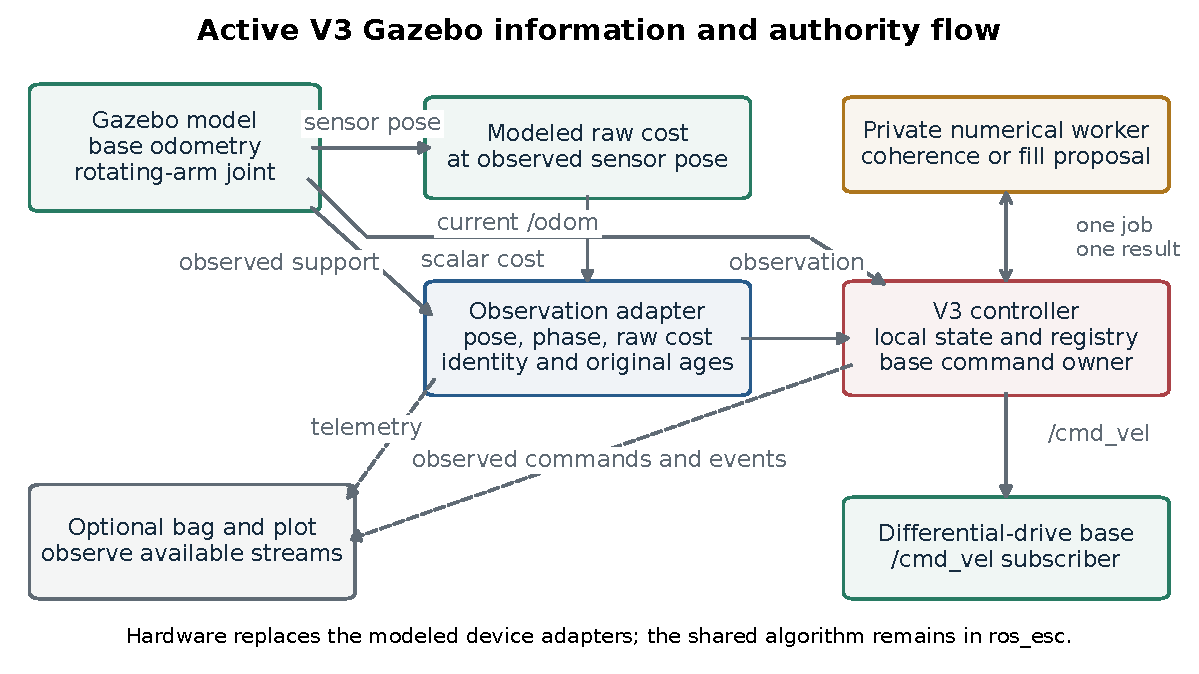
\includegraphics[width=1\linewidth,height=\textheight,keepaspectratio,alt={The active Gazebo route separates measured input, numerical proposals, control authority and optional observation.}]{v3/report_figures/architecture.pdf}
\caption{The active Gazebo route separates measured input, numerical
proposals, control authority and optional observation.}
\end{figure}

\subsection{Canonical topics and their direction of
influence}\label{canonical-topics-and-their-direction-of-influence}

The environment profile uses entity name
\passthrough{\lstinline!turtlebot3!}. Topic names are generated in one
place, \passthrough{\lstinline!profiles.py!}. A reader should
distinguish control inputs, actuator outputs, and observer telemetry:

{\def\LTcaptype{none} % do not increment counter
\begin{longtable}[]{@{}
  >{\raggedright\arraybackslash}p{(\linewidth - 6\tabcolsep) * \real{0.2500}}
  >{\raggedright\arraybackslash}p{(\linewidth - 6\tabcolsep) * \real{0.2500}}
  >{\raggedright\arraybackslash}p{(\linewidth - 6\tabcolsep) * \real{0.2500}}
  >{\raggedright\arraybackslash}p{(\linewidth - 6\tabcolsep) * \real{0.2500}}@{}}
\toprule\noalign{}
\begin{minipage}[b]{\linewidth}\raggedright
Topic
\end{minipage} & \begin{minipage}[b]{\linewidth}\raggedright
Type
\end{minipage} & \begin{minipage}[b]{\linewidth}\raggedright
Producer \(\rightarrow\) consumer
\end{minipage} & \begin{minipage}[b]{\linewidth}\raggedright
Meaning
\end{minipage} \\
\midrule\noalign{}
\endhead
\bottomrule\noalign{}
\endlastfoot
\passthrough{\lstinline!/clock!} & \path|rosgraph_msgs/Clock| & Gazebo
\(\rightarrow\) simulation clock infrastructure/recorder & Simulation
timeline; not a cost sample \\
\passthrough{\lstinline!/odom!} &
\passthrough{\lstinline!nav\_msgs/Odometry!} & Gazebo base plugin
\(\rightarrow\) sensor pose, observation adapter, controller, plot/bag &
Observed robot pose in \passthrough{\lstinline!odom!} \\
\passthrough{\lstinline!/joint\_states!} & \path|sensor_msgs/JointState|
& Gazebo joint publisher \(\rightarrow\) encoder & Observed named
rotating-joint angle \\
\path|/turtlebot3/timekeeper_chatter| &
\passthrough{\lstinline!Timekeeper!} & arm owner \(\rightarrow\) legacy
adapters, observation adapter, controller telemetry & Stable experiment
start-time origin and clock mode \\
\path|/turtlebot3/encoder_chatter| & \path|StampedFloat64MultiArray| &
encoder \(\rightarrow\) arm/sensor pose/observation adapter & One arm
angle, relative acquisition timestamp \\
\path|/turtlebot3/sensor_transform_chatter| &
\path|StampedTransformMultiArray| & sensor pose \(\rightarrow\) modeled
cost & Sensor position/orientation transform(s) \\
\path|/turtlebot3/cost_value_chatter| & \path|StampedFloat64MultiArray|
& modeled cost \(\rightarrow\) observation adapter; original filter;
observers & Raw signed cost, one channel for selected V3 \\
\passthrough{\lstinline!/gesc/observation!} &
\passthrough{\lstinline!SensorObservation!} & adapter \(\rightarrow\) V3
controller/bag & Single assembled raw cost, observed support geometry,
phase, provenance \\
\path|/turtlebot3/filter_value_chatter| &
\path|StampedFloat64MultiArray| & original filter \(\rightarrow\)
original controller, or V3 controller \(\rightarrow\) observers & In V3
an output-only body-direction diagnostic \\
\path|/turtlebot3/control_value_chatter| &
\path|StampedFloat64MultiArray| & controller \(\rightarrow\) observers &
Six command components as diagnostic telemetry \\
\passthrough{\lstinline!/cmd\_vel!} & \path|geometry_msgs/Twist| & sole
base controller \(\rightarrow\) Gazebo base/physical external driver &
Actual base command endpoint \\
\path|/velocity_controller/commands| & \path|std_msgs/Float64MultiArray|
& arm owner \(\rightarrow\) arm joint velocity controller &
Rotating-frame angular velocity \\
\passthrough{\lstinline!/gesc/events!} &
\passthrough{\lstinline!AlgorithmEvent!} & V3 controller \(\rightarrow\)
observers & Candidate/fill/escape/best-source/availability events \\
\passthrough{\lstinline!/gesc/fills!} &
\passthrough{\lstinline!GaussianFill!} & V3 controller \(\rightarrow\)
observers & Committed Gaussian geometry and diagnostics \\
\end{longtable}
}

V3 does not subscribe to its own event or fill telemetry. The registry
and objective are local state, not decisions synchronized through
message acknowledgments. A bag subscriber cannot authorize motion;
losing a plot does not alter control. A best-source message is an event
indicating a raw-evidence comparison, not a command to stop or hold a
source.

\textbf{Sources:} \path|ros2_ws/src/ros_esc/ros_esc/profiles.py| lines
84-98; \path|ros2_ws/src/ros_esc/ros_esc/gesc_v3/node.py| lines 82-100,
160-173, 218-263;
\path|ros2_ws/src/ros_esc/ros_esc/rotate_frame_node/rotate_frame_node_script.py|
lines 28-37; \path|ros2_ws/src/ros_esc/ros_esc/run_tools/record_bag.py|
lines 15-32.

\subsection{All eight custom messages, field by
field}\label{all-eight-custom-messages-field-by-field}

The interface package preserves five original message shapes and adds
one observation contract while retaining two telemetry contracts. Not
every available field is populated in the active publisher. The schema
describes capacity; the publisher source defines actual values and
validity flags.

\subsubsection{The five original
contracts}\label{the-five-original-contracts}

\passthrough{\lstinline!Timekeeper!} has
\passthrough{\lstinline!mode: string!} and \path|start_time: float64|.
Mode is \passthrough{\lstinline!sim time!} or
\passthrough{\lstinline!real time!}. The arm owner publishes the stable
start time at 30 Hz. Encoder/cost/filter/control timestamps are
historically relative to this origin; adding the origin recovers an
absolute algorithm-clock timestamp. It does not carry a sample sequence,
hardware acquisition uncertainty, or a ROS Header.

\passthrough{\lstinline!StampedFloat64!} has
\passthrough{\lstinline!header: string!},
\passthrough{\lstinline!timestamp: float64!}, and
\passthrough{\lstinline!data: float64!}. The header is a textual
description, not \passthrough{\lstinline!std\_msgs/Header!}; it has no
frame identifier or ROS stamp structure. \path|StampedFloat64MultiArray|
has the same descriptive header and timestamp but
\passthrough{\lstinline!data: float64[]!}. The array's shape/meaning
depends on the topic: encoder is \passthrough{\lstinline![phase]!},
selected raw cost is \passthrough{\lstinline![cost]!}, V3 filter
diagnostic is a two-component body direction, and controller diagnostic
is \path|[vx, vy, vz, wx, wy, wz]|. Do not identify it as a
multidimensional layout-aware \path|std_msgs/Float64MultiArray|; this
custom type has no \passthrough{\lstinline!layout!} field.

\passthrough{\lstinline!StampedString!} similarly carries
\passthrough{\lstinline!header!}, relative
\passthrough{\lstinline!timestamp!}, and string
\passthrough{\lstinline!data!}. It is retained for compatibility even
though it is not a mandatory selected V3 stream.
\path|StampedTransformMultiArray| has \passthrough{\lstinline!header!},
\passthrough{\lstinline!timestamp!}, and
\path|geometry_msgs/Transform[] transform_array|. Each Transform has
translation and quaternion rotation for a sensor, but the wrapper itself
supplies no explicit parent/child frames. The selected simulation
configuration supplies the intended odometry-to-sensor geometry.

\textbf{Sources:}
\path|ros2_ws/src/ros_esc_interfaces/msg/Timekeeper.msg| lines 1-14;
\passthrough{\lstinline!StampedFloat64.msg!} lines 1-10;
\path|StampedFloat64MultiArray.msg| lines 1-10;
\passthrough{\lstinline!StampedString.msg!} lines 1-10;
\path|StampedTransformMultiArray.msg| lines 1-13;
\path|ros2_ws/src/ros_esc/ros_esc/rotate_frame_node/rotate_frame_node_script.py|
lines 34-37, 57-61; \path|ros2_ws/src/ros_esc/ros_esc/gesc_v3/node.py|
lines 165-171, 223-227.

\subsubsection{SensorObservation: the control input
contract}\label{sensorobservation-the-control-input-contract}

{\def\LTcaptype{none} % do not increment counter
\begin{longtable}[]{@{}
  >{\raggedright\arraybackslash}p{(\linewidth - 2\tabcolsep) * \real{0.5000}}
  >{\raggedright\arraybackslash}p{(\linewidth - 2\tabcolsep) * \real{0.5000}}@{}}
\toprule\noalign{}
\begin{minipage}[b]{\linewidth}\raggedright
Fields
\end{minipage} & \begin{minipage}[b]{\linewidth}\raggedright
Meaning and actual selected behavior
\end{minipage} \\
\midrule\noalign{}
\endhead
\bottomrule\noalign{}
\endlastfoot
Constants \passthrough{\lstinline!DEVICE\_TIME=0!},
\passthrough{\lstinline!ESTIMATED\_TIME=1!},
\passthrough{\lstinline!RECEIPT\_TIME=2!};
\passthrough{\lstinline!timestamp\_basis!} & Tell the consumer what the
source timestamp represents. Gazebo adapter emits estimated; physical
host acquisition uses receipt basis unless a real device clock
exists. \\
\passthrough{\lstinline!stamp!},
\passthrough{\lstinline!receipt\_stamp!} & ROS Time source and
adapter-receipt timestamps, kept distinct. Completion of an
interpolation or worker job never creates a fresh source timestamp. \\
\passthrough{\lstinline!source\_instance!},
\passthrough{\lstinline!sequence!} & A UUID-like identity for one
adapter lifetime and host sequence incremented for distinct accepted
cost timestamps. A restart creates a new source identity. \\
\path|device_sequence_valid|, \passthrough{\lstinline!device\_sequence!}
& Optional independent device-origin sequence. The generic observation
adapter sets validity false; host counts must not masquerade as an ADC
count. \\
\passthrough{\lstinline!frame\_id!}, \path|source_pose: Pose2D| & Robot
pose at the cost timestamp, supported by nearby observed odometry.
Pose2D contains x, y, theta/yaw. \\
\passthrough{\lstinline!raw\_cost!} & Signed, unaugmented scalar sensor
cost. It remains raw even when control objective changes. \\
\passthrough{\lstinline!phase\_rad!} & Calibrated observed arm phase
relative to the base. It is not nominal RPM multiplied by time. \\
\passthrough{\lstinline!sensor\_x\_m!},
\passthrough{\lstinline!sensor\_y\_m!} & Sensor sample position derived
from base pose, yaw + measured phase, and sensor radius. \\
\path|pose_support_age_sec|, \path|phase_support_age_sec| &
Age/separation of measured support actually used in
interpolation/nearest support. \\
\path|acquisition_uncertainty_sec| & Unknown is NaN. A fabricated zero
would claim a precision that was not measured. \\
\passthrough{\lstinline!valid!}, \passthrough{\lstinline!reason!} &
Whether this record is usable; invalid notices communicate bounded data
rejection or a terminal integrity reason. \\
\end{longtable}
}

The producer uses bounded pose/phase queues, one pending cost record,
and a default 50 ms support tolerance. Exact support is preferred; if
both sides are close it interpolates. If only nearby measured support
exists it uses the nearest support and reports its age. Angular
interpolation uses the shortest wrapped difference, avoiding the
erroneous midpoint across \(\pm\)\(\pi\). This produces
observed/estimated geometry, not simulator truth. Its planar sensor
location is \path|x_sensor = x_base + 0.18 cos(yaw + phase)| and
\path|y_sensor = y_base + 0.18 sin(yaw + phase)| for the selected
radius.

\textbf{Sources:}
\path|ros2_ws/src/ros_esc_interfaces/msg/SensorObservation.msg| lines
1-23; \path|ros2_ws/src/ros_esc/ros_esc/gesc_v3/observation.py| lines
9-35, 58-114;
\path|ros2_ws/src/ros_esc/ros_esc/gesc_v3/observation_node.py| lines
72-92, 237-266; \path|ros2_ws/src/ros_esc/ros_esc/gesc_v3/records.py|
lines 20-50.

\subsubsection{AlgorithmEvent: what telemetry can and cannot tell
you}\label{algorithmevent-what-telemetry-can-and-cannot-tell-you}

The schema defines event constants for configuration/capability/state
transition; candidate/confirmation/verification; fill
created/rejected/merged/superseded/escalated/failed/low-confidence; goal
reached; escape started/stalled; recenter started/completed; timeout and
failsafe. They are retained telemetry labels, not proof that active V3
implements all of the historic states implied by their names.

Fields are \passthrough{\lstinline!stamp!}; optional
\passthrough{\lstinline!source\_timestamp!} and
\path|source_timestamp_valid|; \passthrough{\lstinline!event\_type!};
optional numeric \passthrough{\lstinline!state!}, textual
\passthrough{\lstinline!state\_name!}, and
\passthrough{\lstinline!state\_valid!}; optional
\passthrough{\lstinline!fill\_id!} and
\passthrough{\lstinline!fill\_id\_valid!};
\passthrough{\lstinline!reason\_code!}; human-readable
\passthrough{\lstinline!detail!}; and parallel
\passthrough{\lstinline!value\_names!}/\passthrough{\lstinline!values!}
arrays. The current publisher maps candidate \(\rightarrow\) 10,
fill-created \(\rightarrow\) 20, best-source \(\rightarrow\) 30,
escape-started \(\rightarrow\) 40, and other events \(\rightarrow\)
state-transition 3. It fills \passthrough{\lstinline!state\_name!} with
availability/activity, marks state valid, and emits
\passthrough{\lstinline!detail!} as kind plus reason. It does not
populate an authoritative numeric state enumeration, source timestamp,
fill ID, reason-code catalogue, or the value arrays in this path.
Analysis must therefore read the validity flags and
\passthrough{\lstinline!detail!}, rather than interpret default zeros as
measured facts. Event state text is constructed at publish time, so
\passthrough{\lstinline!detail!} and the core event timestamp are the
primary transition evidence.

\textbf{Sources:}
\path|ros2_ws/src/ros_esc_interfaces/msg/AlgorithmEvent.msg| lines 1-38;
\path|ros2_ws/src/ros_esc/ros_esc/gesc_v3/node.py| lines 229-243;
\path|ros2_ws/src/ros_esc/ros_esc/gesc_v3/records.py| lines 62-67;
\path|ros2_ws/src/ros_esc/ros_esc/run_tools/analyze_bag.py| lines 63-68.

\subsubsection{GaussianFill: a committed geometry
record}\label{gaussianfill-a-committed-geometry-record}

\passthrough{\lstinline!GaussianFill!} carries publish
\passthrough{\lstinline!stamp!}, valid source timestamp, and frame;
identity \passthrough{\lstinline!fill\_id!},
\passthrough{\lstinline!cluster\_id!},
\passthrough{\lstinline!revision!}; center
\passthrough{\lstinline!center\_x!},
\passthrough{\lstinline!center\_y!}; amplitude; covariance entries
xx/xy/yy; principal widths \passthrough{\lstinline!sigma\_major!},
\passthrough{\lstinline!sigma\_minor!}; orientation; support and exit
radii; confidence; sample count; fit residual; condition number; design
escalation count; their corresponding validity flags; and
active/superseded flags. The active publisher fills these from the
committed fill object and marks valid geometry/diagnostics individually;
the condition-number flag is copied from the fit, because a condition
estimate can remain unavailable. Covariance describes Gaussian spatial
shape, not the robot's localization covariance. Confidence is an
implementation diagnostic, not a universal probability of escape
success.

This is output-only telemetry. The control owner commits to its local
registry first; publishing a \passthrough{\lstinline!GaussianFill!}
neither changes a second node's objective nor asks another owner for
approval. The analyst can draw ellipses only when frame and widths are
valid and compatible with the recorded odometry frame.

\textbf{Sources:}
\path|ros2_ws/src/ros_esc_interfaces/msg/GaussianFill.msg| lines 1-37;
\path|ros2_ws/src/ros_esc/ros_esc/gesc_v3/node.py| lines 244-263;
\path|ros2_ws/src/ros_esc/ros_esc/run_tools/analyze_bag.py| lines
266-297.

\subsection{Profiles, parameters, and the exact meaning of a run
command}\label{profiles-parameters-and-the-exact-meaning-of-a-run-command}

\passthrough{\lstinline!resolve\_profile()!} first finds the selected
installed \path|share/ros_esc/config/profiles| directory through the
ament index. Pure source tests can fall back to the source resource
directory. It reads \passthrough{\lstinline!algorithms.json!} and
\passthrough{\lstinline!environments.json!}, deep-copies the selected
algorithm, and resolves exactly five config roles: rotation, sensor,
cost, filter, controller. A custom profile is a JSON file using the same
structure; relative asset paths are resolved against that file's
directory. It accepts only \passthrough{\lstinline!legacy!} or
\passthrough{\lstinline!gesc\_v3!} algorithms, and rejects missing
resources. Built-in objects use importable
\passthrough{\lstinline!module!} references; custom original object JSON
retains \passthrough{\lstinline!filepath!} support.

The environment contributes simulation/physical mode, clock, entity,
frame, plotting default, support rate, and world. The active Gazebo
environment is \passthrough{\lstinline!simulation!}, true simulation
time, entity \passthrough{\lstinline!turtlebot3!}, frame
\passthrough{\lstinline!odom!}, plot true, 30 Hz sensor support, and
\passthrough{\lstinline!gazebo\_empty.world!}. The physical environment
selects wall time and plot false, with no Gazebo world/support-rate
setting. \passthrough{\lstinline!gazebo.launch.py!} explicitly rejects a
physical environment; setting \path|environment:=physical| does not
transform a simulated robot launch into a hardware launch.

One nuance is that resolving a profile is a pure repeatable operation,
not a mutable run configuration broker. The launch resolves its graph,
and the observation/controller nodes also resolve their startup
settings. Gains and caps have a single effective JSON owner, so those
resolutions agree without copying a second set into profile metadata.
Editing a source JSON should be followed by the documented build before
relying on installed resources; runs do not build or rewrite JSON.

The V3 profile declares 5 Hz modeled cost, 20 Hz command cadence, 0.5 s
input expiry, 5 s fill preparation, 4000 maximum fit samples, and 0.18 m
sensor radius. The controller JSON supplies
\passthrough{\lstinline!k\_vx=0.5!}, \passthrough{\lstinline!k\_wz=5!},
Gazebo caps 0.10 m/s and 0.50 rad/s, affine magnitude 2.0, direct escape
assistance false, stall window 15 s, and assistance path 0.20 m.
Physical caps are separately selected as 0.05/0.30; reading generic
simulation resources with environment physical is not sufficient to
apply the physical selected configuration.

Some declared fields deserve precise interpretation. The Gazebo arm's
actual selected commanded speed is owned by
\passthrough{\lstinline!full\_rotation.json!}
(\passthrough{\lstinline!spin\_rpm: 20!}), not by the profile's
\passthrough{\lstinline!arm\_rpm!} label. The profile's 54-degree
encoder offset records the physical selection; Gazebo phases are already
observed joint angles and the generic observation adapter deliberately
applies no such offset. \path|coherence_expiry_sec| is declared as 0.5
in the profile, while the current core explicitly submits coherence jobs
with a 0.5 s timeout rather than exposing that field through
\passthrough{\lstinline!CoreConfig!}. V3 still requires a filter asset
role for compatible profile structure, but does not instantiate that
legacy filter JSON in the V3 graph. These distinctions prevent a
metadata edit from being mistaken for an effective runtime tuning
change.

\textbf{Sources:} \path|ros2_ws/src/ros_esc/ros_esc/profiles.py| lines
8-20, 32-98;
\path|ros2_ws/src/ros_esc/config/profiles/environments.json| lines 1-20;
\path|ros2_ws/src/ros_esc/config/profiles/algorithms.json| lines
178-204;
\path|ros2_ws/src/ros_esc/config/profiles/assets/gesc_v3/controller.json|
lines 1-19; \path|ros2_ws/src/ros_esc/ros_esc/gesc_v3/node.py| lines
49-78; \path|ros2_ws/src/ros_esc/ros_esc/gesc_v3/core.py| lines 447-461;
\path|ros2_ws/src/ros_esc/ros_esc/gesc_v3/observation_node.py| lines
175-193; \path|docs/environment_parameters.md| lines 3-42.

\subsection{Effective startup settings versus source
defaults}\label{effective-startup-settings-versus-source-defaults}

The table distinguishes selected startup values from fallback defaults;
that distinction prevents a reader from treating a dataclass default as
the active Gazebo cap. The complete leaf-level source inventory is in
\path|v3/report_parameters.tsv|.

{\def\LTcaptype{none} % do not increment counter
\begin{longtable}[]{@{}
  >{\raggedright\arraybackslash}p{(\linewidth - 4\tabcolsep) * \real{0.3333}}
  >{\raggedright\arraybackslash}p{(\linewidth - 4\tabcolsep) * \real{0.3333}}
  >{\raggedright\arraybackslash}p{(\linewidth - 4\tabcolsep) * \real{0.3333}}@{}}
\toprule\noalign{}
\begin{minipage}[b]{\linewidth}\raggedright
Setting
\end{minipage} & \begin{minipage}[b]{\linewidth}\raggedright
Selected Gazebo V3
\end{minipage} & \begin{minipage}[b]{\linewidth}\raggedright
Source owner / precedence
\end{minipage} \\
\midrule\noalign{}
\endhead
\bottomrule\noalign{}
\endlastfoot
\passthrough{\lstinline!profile!}, \passthrough{\lstinline!environment!}
& \passthrough{\lstinline!gesc\_v3!}, \passthrough{\lstinline!gazebo!} &
Launch arguments forwarded as ROS parameters; selected profile resolved
at startup \\
\passthrough{\lstinline!use\_sim\_time!} & true & Environment profile;
explicit override must agree or startup rejects it \\
\path|direct_escape_assistance_enabled| & false & Controller JSON seeds
the declared ROS Boolean parameter; an explicit ROS startup override can
select true \\
\passthrough{\lstinline!k\_vx!}, \passthrough{\lstinline!k\_wz!} & 0.5,
5.0 & Selected controller JSON gains \\
\passthrough{\lstinline!max\_vx!}, \passthrough{\lstinline!max\_wz!} &
0.10 m/s, 0.50 rad/s & Selected controller JSON params; CoreConfig
fallback defaults are 0.05/0.30 \\
\path|escape_affine_magnitude| & 2.0 & Controller JSON; older omitted
profiles fall back to 0.5 \\
\path|escape_assist_stall_window_sec|, \path|escape_assist_distance_m| &
15 s, 0.20 m & Controller JSON; switch false means direct assistance
remains disabled \\
\passthrough{\lstinline!input\_expiry!},
\passthrough{\lstinline!control\_hz!} & 0.5 s, 20 Hz & Profile values
copied into CoreConfig \\
\path|preparation_timeout|, \passthrough{\lstinline!maximum\_snapshot!}
& 5 s, 4000 & Profile fill budget / maximum fit sample cap \\
\passthrough{\lstinline!sensor\_radius!} & 0.18 m & Profile
\(\rightarrow\) observation geometry and CoreConfig GESC arm length \\
\passthrough{\lstinline!washout\_omega!} & 1.0 & CoreConfig default
retained by node construction \\
\passthrough{\lstinline!candidate\_radius!} & 0.75 m & CoreConfig
default retained by node construction \\
\passthrough{\lstinline!maximum\_history!} & 20000 & CoreConfig default;
bounded raw evidence and pose history \\
observation \passthrough{\lstinline!support\_tolerance!},
\passthrough{\lstinline!capacity!} & 0.05 s, 256 each &
ObservationBuilder constructor defaults \\
clock delivery \passthrough{\lstinline!max\_lead!},
\passthrough{\lstinline!capacity!} & 0.125 s, 32 per stream &
ClockDelivery defaults; expiry inherited from selected input expiry \\
phase/odometry support & 30 Hz configured & Environment \(\rightarrow\)
joint publisher; base drive plugin publishes odometry at 30 Hz \\
raw modeled cost & at most 5 Hz & Profile \(\rightarrow\) cost node CLI
rate limiter on distinct transforms \\
coherence numerical-job deadline & 0.5 s & Explicit core submit call;
profile metadata matches but is not separately wired \\
arm-manager update rate & 100 Hz & \path|joint_controller.yaml| \\
arm speed & 20 RPM nominal & Selected full\_rotation JSON
\(\rightarrow\) constant spin-profile object \\
\end{longtable}
}

V3 uses only three declared ROS selections in its controller shell
besides the standard clock parameter: profile, environment, and
direct-assistance enabled. Other numerical values are resolved
JSON/profile fields or code configuration objects; they do not become
arbitrary ROS parameters simply because their names appear in a report.
Original controller/filter use strict
\passthrough{\lstinline!--use-sim-time!} CLI arguments instead of
accepting appended ROS \passthrough{\lstinline!-p!} arguments. The
generic shared clock helper preserves an explicit startup override when
legacy simulation adapters are constructed, rather than globally
rewriting defaults according to the machine storing source.

\textbf{Sources:} \path|ros2_ws/src/ros_esc/ros_esc/gesc_v3/node.py|
lines 49-78; \path|ros2_ws/src/ros_esc/ros_esc/gesc_v3/records.py| lines
70-108; \path|ros2_ws/src/ros_esc/ros_esc/gesc_v3/observation.py| lines
21-35; \path|ros2_ws/src/ros_esc/ros_esc/gesc_v3/clock_delivery.py|
lines 28-33; \path|ros2_ws/src/ros_esc/ros_esc/gesc_v3/core.py| lines
447-461; \path|ros2_ws/src/ros_esc/ros_esc/clock_configuration.py| lines
6-43;
\path|ros2_ws/src/ros_esc/ros_esc/controller_node/controller_node_script.py|
lines 38-44, 220-228;
\path|ros2_ws/src/ros_esc/ros_esc/filter_node/filter_node_script.py|
lines 32-40.

\subsection{The 19 aliases and what they actually
select}\label{the-19-aliases-and-what-they-actually-select}

Every Bash wrapper is a short explicit alias for
\path|ros2 launch turtlebot3_rotating_sensor gazebo.launch.py profile:=NAME|,
forwarding additional launch arguments. Their names remain selectable
for original-method continuity. They select installed resources and
perform no build. The profile table below describes actual objects
rather than inferring behavior from filenames.

{\def\LTcaptype{none} % do not increment counter
\begin{longtable}[]{@{}
  >{\raggedright\arraybackslash}p{(\linewidth - 6\tabcolsep) * \real{0.2500}}
  >{\raggedright\arraybackslash}p{(\linewidth - 6\tabcolsep) * \real{0.2500}}
  >{\raggedright\arraybackslash}p{(\linewidth - 6\tabcolsep) * \real{0.2500}}
  >{\raggedright\arraybackslash}p{(\linewidth - 6\tabcolsep) * \real{0.2500}}@{}}
\toprule\noalign{}
\begin{minipage}[b]{\linewidth}\raggedright
Profile / alias basename
\end{minipage} & \begin{minipage}[b]{\linewidth}\raggedright
Controller family
\end{minipage} & \begin{minipage}[b]{\linewidth}\raggedright
Cost
\end{minipage} & \begin{minipage}[b]{\linewidth}\raggedright
Rotation
\end{minipage} \\
\midrule\noalign{}
\endhead
\bottomrule\noalign{}
\endlastfoot
\path|adagrad_bnf_rotation_acoustic| & Rotating directional + AdaGradODE
& Acoustic expression & Back/forth, acoustic rotation config \\
\path|adagrad_bnf_rotation_resistance| & Rotating directional +
AdaGradODE & Photoresistor resistance & Back/forth \\
\path|adagrad_bnf_rotation_voltage| & Rotating directional + AdaGradODE
& Negative photoresistor voltage & Back/forth \\
\path|adagrad_full_rotation_acoustic| & Rotating directional +
AdaGradODE & Acoustic expression & Full rotation, acoustic config \\
\path|adagrad_full_rotation_resistance| & Rotating directional +
AdaGradODE & Photoresistor resistance & Full rotation \\
\path|adagrad_full_rotation_voltage| & Rotating directional + AdaGradODE
& Negative photoresistor voltage & Full rotation \\
\passthrough{\lstinline!angular\_tuning!} &
\path|Angular_Velocity_Input_Controller| & Negative photoresistor
voltage & No arm rotation (Constant\_Full\_Rotation, 0 RPM) \\
\passthrough{\lstinline!forward\_tuning!} &
\path|Forward_Velocity_Input_Controller| & Negative photoresistor
voltage & No arm rotation (Constant\_Full\_Rotation, 0 RPM) \\
\path|gesc_bnf_rotation_acoustic| & Directional\_Controller & Acoustic
expression & Back/forth, acoustic config \\
\path|gesc_bnf_rotation_voltage| & Directional\_Controller & Negative
photoresistor voltage & Back/forth \\
\path|gesc_full_rotation_acoustic| & Directional\_Controller & Acoustic
expression & Full rotation, acoustic config \\
\passthrough{\lstinline!gesc\_v3!} & V3Core + Directional\_Controller &
Multi-light negative voltage & Full rotation, 20 RPM \\
\passthrough{\lstinline!hb\_acoustic!} &
\textbf{\path|Forward_Velocity_Input_Controller|} & Acoustic expression
& Full-rotation config \\
\path|hbesc_full_rotation_voltage| & Rotating directional + HeavyBallODE
& Negative photoresistor voltage & Full rotation \\
\passthrough{\lstinline!lie\_bracket!} & Lie\_Bracket\_Controller &
Negative photoresistor voltage & Constant\_Full\_Rotation object with
zero RPM in \passthrough{\lstinline!no\_rotation.json!} \\
\path|rmsprop_bnf_rotation| & Rotating directional + RMSPropODE &
Photoresistor resistance & Back/forth \\
\path|rmsprop_bnf_rotation_acoustic| & Rotating directional + RMSPropODE
& Acoustic expression & Generic back/forth config \\
\path|rmsprop_full_rotation| & Rotating directional + RMSPropODE &
Quadratic expression & Full rotation \\
\path|rmsprop_full_rotation_acoustic| & Rotating directional +
RMSPropODE & Acoustic expression & Generic full-rotation config \\
\end{longtable}
}

\passthrough{\lstinline!hb\_acoustic!} is a historical alias label; it
does not currently select HeavyBallODE. Likewise the acoustic RMSProp
aliases reuse generic controller/rotation resources while changing the
cost. This report describes the current code faithfully and does not
silently rename or repair retained recipes. V3's low-rate,
recurrent-verification/Gaussian method is a separate selected runtime,
not an automatic upgrade applied to every original alias.

\textbf{Sources:}
\path|ros2_ws/src/ros_esc/config/profiles/algorithms.json| lines 2-317;
all nineteen files in
\path|ros2_ws/src/turtlebot3_rotating_sensor/bash_scripts/{adaptive_methods,gradient_methods,accelerated_methods}|
(lines 1-5 in each);
\path|ros2_ws/src/ros_esc/config/profiles/assets/ros_esc/rotate_frame_node/rotate_frame_config_files/turtlebot_vehicle/no_rotation.json|
lines 1-9. An exact asset/parameter inventory accompanies this report as
\path|v3/report_parameters.tsv|.

\subsection{Robot model, kinematics, and what Gazebo
simulates}\label{robot-model-kinematics-and-what-gazebo-simulates}

The model is a TurtleBot differential-drive base with a rotating
horizontal sensor arm. \passthrough{\lstinline!base\_footprint!} is the
planar reference, \passthrough{\lstinline!base\_link!} is 0.010 m above
it, the rotating joint is 0.355 m above the base link, and the sensor is
0.18 m outward with a 0.015 m vertical offset from the arm. The rotating
joint is continuous about z; selected initial phase is zero. The base
collision model is a simple 0.140 \(\times\) 0.140 \(\times\) 0.33 m
box, not a exact mechanical CAD reconstruction. Wheel collision radius
is 0.033 m; a low-friction fixed sphere approximates the caster. Meshes
supply appearance; collisions/inertias supply physics. CAD/print files
are useful mechanical assets, not runtime algorithm code.

The Gazebo differential-drive plugin consumes
\passthrough{\lstinline!/cmd\_vel!}, publishes
\passthrough{\lstinline!/odom!} and odometry transform at 30 Hz, and
uses 0.160 m wheel separation and 0.066 m diameter. The controller
object's hardware-limit calculation has wheel distance 0.158 m in the
selected JSON. That small distinction is explicit in source and should
not be erased in an explanation. With selected cap overrides it does not
set the 0.10/0.50 velocity limits; those limits come directly from JSON.
Ideal planar kinematics are
\passthrough{\lstinline!x\_dot = v cos(yaw)!},
\passthrough{\lstinline!y\_dot = v sin(yaw)!},
\passthrough{\lstinline!yaw\_dot = w!}. Differential drive realizes them
through left/right wheel rates. Reverse signed
\passthrough{\lstinline!v!} is valid and can reduce turning
requirements; the controller does not require forward-only translation.

The arm uses ros2\_control's \path|JointGroupVelocityController|; it is
distinct from the base's Gazebo differential-drive plugin. Its YAML runs
the controller manager at 100 Hz and exposes the rotating joint velocity
command/position/velocity state. The constant-full-rotation object
converts 20 RPM to \path|20 * 2pi/60 approximately 2.094 rad/s|. A 3 s
nominal rotation at 5 cost samples/s yields about 15 samples per turn.
These are nominal settings; the algorithm uses observed phase, and bag
analysis reports measured angular travel rather than assuming perfect
tracking.

The general sensor-pose adapter computes a homogeneous transform
\path|T_odom,sensor = T_odom,base T_base,joint(phase) T_joint,sensor|.
Translation and quaternion orientation are encoded into
\path|StampedTransformMultiArray|. The modeled cost therefore depends
both on sensor position and facing direction. For V3's control input,
the observation adapter independently assembles the measured base
pose/phase at the cost source stamp and computes the planar sample
position. The modeled sensor-pose path currently uses latest received
odometry when an encoder callback arrives; the observation contract
records nearby pose/phase support and its age, rather than claiming
exact simulator ground truth at each acquisition.

The active environment world is
\passthrough{\lstinline!gazebo\_empty.world!}, containing the sun and
ground plane. The visible selected source markers are spawned from the
selected cost JSON; they are visual scene assets, not brightness
measurements from a camera or ray-traced photoresistor. Historical
bounded-world SDF files remain available, but the active environment
does not select them automatically. Neither the robot's lidar/IMU model
nor optional contact telemetry is a source-seeking input to V3. There is
no obstacle navigation stack or SLAM-based global plan in this selected
algorithm graph.

\textbf{Sources:}
\path|ros2_ws/src/turtlebot3_rotating_sensor/urdf/turtlebot3_rotating_sensor.urdf|
lines 11-55, 253-335, 349-418, 423-505;
\path|ros2_ws/src/turtlebot3_rotating_sensor/controller_config/joint_controller.yaml|
lines 1-19;
\path|ros2_ws/src/ros_esc/config/profiles/assets/ros_esc/sensor_pose_node/transform_config_files/turtlebot_rotating_sensor.json|
lines 1-44;
\path|ros2_ws/src/ros_esc/ros_esc/sensor_pose_node/transform_objects/transform_objects.py|
lines 63-104, 107-198; \path|sensor_pose_node_script.py| lines 40-65;
\path|ros2_ws/src/ros_esc/ros_esc/rotate_frame_node/spin_profile_objects/spin_profile_objects.py|
lines 65-97;
\path|ros2_ws/src/turtlebot3_rotating_sensor/worlds/gazebo_empty.world|
lines 1-12; \path|launch/gazebo.launch.py| lines 56-74;
\path|ros2_ws/src/ros_esc/config/profiles/assets/gesc_v3/controller.json|
lines 8-17.

\subsection{Cost models and minimization
sign}\label{cost-models-and-minimization-sign}

Every selected method solves a minimization problem. For light-voltage
seeking, a brighter measurement has larger positive physical voltage but
more negative cost. The modeled voltage cost is
\passthrough{\lstinline!J = -5/(R/330 + 1)!} volts. Lower resistance or
brighter illumination therefore lowers J. A positive Gaussian bump added
to J raises a previously attractive low region; the control still
minimizes the resulting objective. This sign convention is essential
when describing filling: the algorithm does not reward the old minimum
with a larger negative well.

The single-light \path|Photoresistor_Interpolated_Map| computes radial
distance r and facing error \(\beta\) (degrees), evaluates an empirical
quadratic resistance fit
\path|R = a r^2 + b beta^2 + c rbeta + d r + e beta + f|, clips to
{[}100, 337260{]} \(\Omega\), optionally approximates ADC quantization,
and returns resistance or negative divider voltage. The coefficients are
\passthrough{\lstinline!a=8280.82113!},
\passthrough{\lstinline!b=7.90425287!},
\passthrough{\lstinline!c=442.130406!}, with very small d/e/f terms.
This is a directional fitted surrogate, not a universal inverse-square
illumination law or hardware calibration valid for every
sensor/environment.

The selected V3 \path|Multi_Light_Source_Cost| uses that same
directional curve for each source but combines them in
\textbf{conductance}, rather than adding voltages or taking a
nearest-source minimum. Let
\passthrough{\lstinline!G\_dark = 1/337260!}. For source i,
\path|DeltaG_i = max(1/R_i - G_dark, 0) I_i/I_reference|. Then
\path|G_total = G_dark + SigmaDeltaG_i|,
\path|R_total = clip(1/G_total, 100, 337260)|, and voltage mode applies
the negative divider conversion. This creates a spatial/directional
multi-source landscape from which local minima can arise. Intensity
scales the source's incremental conductance. Zero-intensity sources
contribute zero.

The current built-in scene contains a weaker source at
\path|(0.5740251485, 1.3858192988)| with 400 lumens and a stronger
source at \passthrough{\lstinline!(3.5,3.5)!} with 1600 lumens,
reference 1000 lumens, scale 1, ADC false, and
\passthrough{\lstinline!No\_Noise!}. New source configurations also
support brightness percentages through the brightness helper, while this
selected asset still uses legacy lumen values. Source
positions/strengths belong to modeled acquisition and visualization, not
to \passthrough{\lstinline!SensorObservation!} or the control core. The
core cannot ask the simulator which source is globally best.

Original acoustic/quadratic profiles use
\path|Position_Based_Sympy_Expression|: configured expressions are
converted into executable mathematical functions. Their units and
interpretation belong to the selected expression and must not be equated
with negative volts simply because the same topic carries both. The
noise object is another configured component: no noise, uniform noise,
Gaussian noise, or a configured user-defined time expression can be
selected. The selected V3 cost adapter rate-limits fresh sensor
transforms to at most 5 Hz; skipped or duplicate timestamps produce no
synthetic cost sample.

\textbf{Sources:}
\path|ros2_ws/src/ros_esc/ros_esc/cost_function_node/cost_function_objects/cost_function_objects.py|
lines 66-109, 111-181, 230-267, 282-319, 323-404, 457-560;
\path|ros2_ws/src/ros_esc/config/profiles/assets/gesc_v3/cost.json|
lines 1-28;
\path|ros2_ws/src/ros_esc/ros_esc/cost_function_node/cost_function_node_script.py|
lines 18-65;
\path|ros2_ws/src/ros_esc/ros_esc/cost_function_node/light_brightness.py|
lines 1-76; \path|cost_function_objects/noise_objects.py| lines 1-226.

\subsection{How the original numerical pipeline fits
together}\label{how-the-original-numerical-pipeline-fits-together}

The original configurable filter architecture is a tree of filters
described by JSON. \passthrough{\lstinline!CascadeFilter!} passes one
filter's output into the next; \passthrough{\lstinline!ParallelFilter!}
applies each branch to the same input and concatenates outputs; explicit
FunctionFilter selections route individual components inside branches.
\passthrough{\lstinline!FunctionFilter!} handles algebraic expressions
without a dynamic state; \passthrough{\lstinline!WashoutFilter!} removes
slow/DC components through \path|z_dot = omega (y-z)|, output
\passthrough{\lstinline!y-z!}. Low-pass, Riccati, convolution, and
directional filter classes provide other reusable building blocks. The
config parser recursively instantiates this tree and concatenates each
block's initial state. SymPy translates symbolic expressions, and
retained simple \passthrough{\lstinline!u[...]!} expressions are
evaluated through the original function parser.

The full-rotation GESC filter receives \path|[cost, measured_phase]|,
separates the cost from phase, washouts the cost, computes phase basis
\path|[2 cos(phase)/d, 2 sin(phase)/d]| at d=0.18, and multiplies by
negative washout output. Its two outputs are a descent direction in the
robot frame. Back/forth rotation uses different centered basis
coefficients because a semicircular perturbation does not have the same
zero-mean/full-circle averages. Adaptive methods generate two gradient
components plus three independent components of a symmetric gradient
outer-product estimate, not only the two GESC channels.

The filter ROS node advances its ODE using the original pre-step output
ordering and explicit Euler/refinement logic. An ordinary valid one-step
path is retained; invalid state candidates retry subdivisions from the
original state under a \textbf{64-total-derivative-evaluation budget}.
Exhaustion drops the sample and resets state rather than publishing a
partially integrated result or blocking indefinitely. Input cost/encoder
timestamps must be finite, fresh, and increasing. A large input gap
resets the dynamic filter state.

The controller API is
\path|controller_output(time, state, input_values)| and returns six
components \path|[vx,vy,vz,wx,wy,wz]|. \passthrough{\lstinline!state!}
is \path|[x,y,z,roll,pitch,yaw]|. \path|Directional_Controller| applies
\passthrough{\lstinline!vx=k\_vx*d\_body\_x!},
\passthrough{\lstinline!wz=k\_wz*d\_body\_y!}, then signed caps. The x
component drives along the robot's heading; y does not command
impossible sideways motion, but steers the heading through angular
velocity. This is why a two-dimensional direction can control a
nonholonomic differential-drive base.

\path|Rotating_Frame_Directional_Controller| adds persistent numerical
optimizer state. It rotates observed gradient and gradient-product
estimates from robot frame to world frame, advances the selected ODE,
and rotates the resulting direction back to robot frame. RMSProp tracks
smoothed squared-gradient scale; AdaGrad uses a matrix gradient
outer-product state; HeavyBall tracks momentum with damping. Integrating
in world coordinates avoids treating turning robot axes as fixed
physical directions. The first controller sample takes dt=0 to avoid an
artificial startup jump. The HeavyBall adapter's
\passthrough{\lstinline!input\_gain!} explicitly handles whether its
incoming filter gives gradient or descent direction.

Forward tuning, angular tuning, and Lie-bracket original methods retain
distinct direct control formulas. Forward tuning commands sinusoidally
perturbed linear motion with constant angular speed; angular tuning
fixes linear velocity and modulates turning; Lie-bracket retains its
original implemented angular law. Those direct formulas should be
described from source, not replaced by a textbook method that happens to
share the name. The original controller adapter now consumes only the
first cost component for Lie-bracket's scalar API; other/custom
controllers retain vector input. Retaining these implementations lets V3
be understood against the earlier baseline without implying that all
legacy profiles share V3's observation joins, numerical worker, or
Gaussian logic.

\textbf{Sources:}
\path|extremum-seeking/src/extremum_seeking/filters/base_filters.py|
lines 215-284, 380-496; \path|filters/aggregate_filters.py| lines
20-204, 205-341; \path|ros2_ws/src/ros_esc/ros_esc/config_parsing.py|
lines 69-235, 301-383, 433-494;
\path|ros2_ws/src/ros_esc/ros_esc/filter_node/filter_node_script.py|
lines 17-70, 93-153; selected
\path|assets/ros_esc/filter_node/filter_config_files/turtlebot_vehicle/gradient_methods/gesc_filter_full_rotation.json|
lines 1-67; \path|controller_objects/turtlebot_vehicle.py| lines 64-172,
178-338, 407-431, 499-527, 595-619;
\path|controller_objects/turtlebot_ode_objects.py| lines 71-190,
192-315, 317-414; \path|controller_node_script.py| lines 164-179.

\subsection{V3 ownership, availability, and private
worker}\label{v3-ownership-availability-and-private-worker}

V3 has two different kinds of state. \textbf{Availability} answers
whether control can currently use essential inputs:
\passthrough{\lstinline!ACTIVE!}, recoverable
\passthrough{\lstinline!WAITING\_INPUT!}, or terminal
\passthrough{\lstinline!STOPPED!}/\passthrough{\lstinline!FAULTED!}.
\textbf{Research activity} describes what the local algorithm is doing:
search, verify, design, or escape. A failed fit is a research failure,
while missing fresh pose/direction is an availability problem. Treating
both as a generic terminal failsafe would incorrectly turn an optional
numerical failure into permanent loss of basic control.

\passthrough{\lstinline!V3Controller!} is the ROS shell;
\passthrough{\lstinline!V3Core!} owns all algorithm state. The core
holds the measured pose and observation, fresh receipt ages,
instantaneous and rolling GESC, recurrent detector, moving evidence,
registry, objective revision, candidate identity, search epoch, affine
terms, and escape progress. It knows neither ROS graph metadata nor a
recorder, simulator field, or device driver. The ROS shell performs
conversion/transport, runs a 20 Hz steady tick, publishes commands, and
emits optional diagnostics. There is one command endpoint and one
registry commit authority.

Accepted pose source age, observation source age, observation ROS
receipt age, and original local monotonic receipt age must each remain
within 0.5 s. Admission also requires increasing pose timestamps,
increasing observation sequence and timestamp, compatible frame, and
pose/phase support separation at most 0.05 s.
Invalid/duplicate/future/old records are rejected without renewing those
ages. Changing producer identity discards temporal evidence and pending
candidate work and starts a new epoch. It preserves an already committed
ESCAPE fill, direction and affine term with its original age; recently
retired IDs are rejected so a delayed old stream cannot reclaim
ownership. A frozen \passthrough{\lstinline!/clock!} still lets the
steady timer expire held commands. New fresh usable inputs can
automatically return \passthrough{\lstinline!WAITING\_INPUT!} to
\passthrough{\lstinline!ACTIVE!}, while Ctrl+C and actual
integrity/ownership/actuator faults remain terminal.

The owner starts on the first \textbf{usable} direction and fresh pose,
not on a full rotation, completed fit, or recorder ready signal. The
initial cost primes washout state: a single brightness level is not a
measured gradient. Numerical coherence can improve direction evidence
later without withholding basic control until a worker completes. During
verification/design the controller commands moving approach/probing; no
internal elapsed candidate deadline exists while valid geometry,
translating motion, and fresh input continue. Design itself has a finite
5 s preparation budget, and failure cancels only that candidate.

The numerical worker uses multiprocessing's \textbf{spawn} context and
capacity-one request/result channels. Only one job may be in flight;
work does not accumulate behind it. Immutable job keys carry type and
identities. A coherence key contains epoch, objective revision, and
source stamp; a fill key adds candidate identity and registry
generation. The main core rejects mismatched, expired, or context-stale
results. Completing a fit does not grant permission to commit into a
changed candidate or registry. Coherence has a 0.5 s job timeout; fill
preparation uses 5 s; fit snapshot is capped at 4000 records. These
finite numerical budgets differ from operator run duration or
verification collection time.

The child has no ROS publisher, actuator access, or live registry
authority. It returns a proposal/result or error; exceptions are data.
On expiry/death the parent retires/restarts the child, polls without
waiting, and continues fresh basic control. Fill/objective changes are
committed at a subsequent new real observation, so old direction history
is not relabeled under a new objective. The core resets relevant
direction history and waits for a real sample of the new objective
rather than replaying old measurements as new acquisitions.

\textbf{Sources:} \path|ros2_ws/src/ros_esc/ros_esc/gesc_v3/node.py|
lines 46-101, 111-173, 186-216; \passthrough{\lstinline!core.py!} lines
1-6, 47-117, 119-235, 447-485, 548-580;
\passthrough{\lstinline!worker.py!} lines 15-29, 39-146;
\passthrough{\lstinline!records.py!} lines 70-108.

\subsection{Clock catch-up, ownership checks, and
shutdown}\label{clock-catch-up-ownership-checks-and-shutdown}

Gazebo's independently delivered clock and sensor topics can arrive in
an inconvenient order. \passthrough{\lstinline!ClockDelivery!} allows a
small, bounded holding area: at most 32 records, source lead \(\leq\)125
ms, and the same 0.5 s source/steady expiry. A sample is not usable
until the clock has caught up to its source/availability time. The queue
never rewrites the sample timestamp. Duplicates are rejected before
queuing. This solves delivery order while preserving the rule that
future data cannot authorize motion; it is not a looser freshness
threshold.

The ROS shell checks publisher count on
\passthrough{\lstinline!/cmd\_vel!} once per steady second. An observed
competing publisher causes a terminal ownership fault. If graph metadata
itself is unavailable, it warns rather than converting
recording/plotting/subscriber availability into a motion gate. This is a
periodic diagnostic, not a proof that no competing command could exist
between checks. Actual actuator publish failure faults and makes a
best-effort zero through the command endpoint. Optional telemetry
failures only warn.

Orderly Ctrl+C/SIGTERM handling defers repeated signals through
final-zero and worker/executor cleanup. \passthrough{\lstinline!stop()!}
cancels the command timer, latches core
\passthrough{\lstinline!STOPPED!}, publishes final zero, then closes the
numerical worker and process lease. The arm owner similarly latches
stopped and publishes arm neutral. The optional recorder waits a short
tail before closing its own bag process, allowing final commands to
reach the recording. Recorded zero is evidence of a command publication,
not proof of measured floor stopping.

\passthrough{\lstinline!process\_lease.py!} is shared support for the
separately managed physical runtime. Gazebo normally has no lease.
Physical environment variables may bind the controller/acquisition to a
Pi-local guard through Unix datagram sockets; a controller tick is sent
only after successful command publication. The lease tracks completed
local process progress and reciprocal guard acknowledgment, not ROS
sensor freshness, recorder readiness, numerical success, run duration,
or SSH connectivity. Linux parent-death binding also kills an orphaned
numerical child/driver when its actual parent disappears. The
guard/physical driver are outside this checkout. A leased terminal
controller fault exits toward the guard's critical-child stop path;
\passthrough{\lstinline!WAITING\_INPUT!} keeps renewing local progress
while commanding zero and can recover. These software mechanisms still
require physical operator evidence for actual stopping behavior.

\textbf{Sources:}
\path|ros2_ws/src/ros_esc/ros_esc/gesc_v3/clock_delivery.py| lines
17-62; \passthrough{\lstinline!node.py!} lines 146-158, 175-216,
265-300; \passthrough{\lstinline!process\_lease.py!} lines 1-7, 18-31,
34-111, 121-128;
\path|ros2_ws/src/ros_esc/ros_esc/deferred_signal_shutdown.py| lines
1-40; \path|rotate_frame_node_script.py| lines 63-88;
\path|run_tools/record_bag.py| lines 35-71.

\subsection{Optional plotting, standard recording, and honest offline
analysis}\label{optional-plotting-standard-recording-and-honest-offline-analysis}

Interactive Gazebo automatically opens the familiar Matplotlib layout: x
position, y position, scalar-cost history, and planar trajectory. The
\passthrough{\lstinline!3D!} display option uses z-history in place of
planar trajectory. The display process subscribes to odometry/cost,
stores bounded numerical buffers, and updates artists on the GUI thread;
its subscription executor runs separately. No display on the host causes
a graceful skip; plot close/import/display/subscription failures do not
control motion. The GUI enable flag also governs plotting:
\passthrough{\lstinline!gui:=false!} makes plotting false even if a user
explicitly requests \passthrough{\lstinline!plot:=true!}. The live
display is a learning/operator aid, not complete archived experiment
evidence.

The optional recorder invokes ordinary
\passthrough{\lstinline!ros2 bag record!} with SQLite storage. Default
topics are \passthrough{\lstinline!/odom!}, encoder, raw cost, filter
diagnostic, \passthrough{\lstinline!/cmd\_vel!},
\passthrough{\lstinline!/gesc/observation!},
\passthrough{\lstinline!/gesc/events!},
\passthrough{\lstinline!/gesc/fills!}, plus
\passthrough{\lstinline!/clock!} in simulation. The timekeeper, sensor
transform, arm command, and control diagnostic are not in this compact
default list; add topics explicitly if a particular analysis needs them.
The recorder does not use \passthrough{\lstinline!--use-sim-time!}: it
records \passthrough{\lstinline!/clock!} but retains the bag transport
timestamp convention. No project-specific manifest or recorder-ready
topic is required. Recorder failure prints a warning and returns without
changing control.

\passthrough{\lstinline!analyze\_bag!} discovers types from ordinary bag
metadata, decodes supported messages, preserves bag time separately from
source time, and reports unknown/missing metrics as null/unavailable. It
reports cadence, duplicate/regressing source timestamps, observed
displacement/path length, final recorded command zero, event counts,
fill records, and measured phase travel. Angle-based RPM uses wrapped
increments; it cannot infer unobserved extra revolutions between sparse
samples. When the encoder topic is absent, an observation-only bag can
supply RPM under explicit adjacent-compatible-pair rules. It never
infers an ADC timestamp or turns requested 20 RPM into measured 20 RPM.

Offline plots use the recorded trajectory and valid same-frame Gaussian
widths. Ellipses show one-sigma principal dimensions; they are not
support or exit circles. Cost/control signal plots use elapsed
\textbf{bag receipt} time, not falsely aligned legacy-relative and
absolute source times. Optional CSV export uses URL-encoded topic
filenames. Nonfinite numeric fields become JSON null. A new analysis
directory is required; the tool refuses to overwrite an existing output.
Missing Matplotlib permits a numeric summary with a warning. Analysis
does not establish source arrival/global optimality merely from a low
raw cost or a \passthrough{\lstinline!best\_source!} event, and does not
establish measured stopping from final zero commands.

\textbf{Sources:}
\path|ros2_ws/src/ros_esc/ros_esc/data_collection_node/data_collection_node_script.py|
lines 10-97; \path|live_plot_animation.py| lines 10-41, 46-138, 141-180;
\path|run_tools/record_bag.py| lines 15-32, 35-99;
\path|run_tools/analyze_bag.py| lines 23-113, 116-191, 203-263, 266-365;
\path|ros2_ws/src/turtlebot3_rotating_sensor/launch/gazebo.launch.py|
lines 82-85, 120-129.

\subsection{Build, run, inspect, and analyze without
guessing}\label{build-run-inspect-and-analyze-without-guessing}

These commands are documented reproduction instructions; this report
preparation did not launch Gazebo or hardware. Use one fresh
terminal/selected overlay. Installing the numerical library is separate
from colcon:

\begin{lstlisting}[language=bash]
cd /home/mattb/dsim-lab
source /opt/ros/humble/setup.bash
timeout 120s python3 -m pip install --user --no-deps -e ./extremum-seeking
cd ros2_ws
timeout 300s colcon build --symlink-install \
  --packages-select ros_esc_interfaces ros_esc turtlebot3_rotating_sensor
source install/setup.bash
\end{lstlisting}

In subsequent terminals:

\begin{lstlisting}[language=bash]
source /opt/ros/humble/setup.bash
source /home/mattb/dsim-lab/ros2_ws/install/setup.bash
\end{lstlisting}

A bounded interactive V3 learning run keeps both Gazebo GUI and plot:

\begin{lstlisting}[language=bash]
timeout --foreground --signal=INT --kill-after=15s 300s \
  ros2 launch turtlebot3_rotating_sensor gazebo.launch.py \
  profile:=gesc_v3 gui:=true plot:=auto record:=true
\end{lstlisting}

The ordinary launch itself has no run-duration deadline and continues
until Ctrl+C. The outer timeout above is an operator/testing bound, not
a convergence gate. The six active launch options are
\passthrough{\lstinline!profile!} (default
\passthrough{\lstinline!gesc\_v3!}),
\passthrough{\lstinline!environment!}
(\passthrough{\lstinline!gazebo!}), \passthrough{\lstinline!gui!}
(\passthrough{\lstinline!true!}), \passthrough{\lstinline!plot!}
(\passthrough{\lstinline!auto!}), \passthrough{\lstinline!record!}
(\passthrough{\lstinline!true!}), and \passthrough{\lstinline!output!}
(\passthrough{\lstinline!\~/Experiments/ESC!}). For example, a bounded
headless software-development run can select
\path|gui:=false plot:=false record:=false|. A Bash alias is equivalent
profile selection, such as \path|bash gradient_methods/gesc_v3.bash|
from the package \passthrough{\lstinline!bash\_scripts!} directory.
Choose one algorithm graph at a time.

Read-only inspection of an already running simulation can illuminate the
architecture:

\begin{lstlisting}[language=bash]
timeout 10s ros2 node list
timeout 10s ros2 topic list -t
timeout 10s ros2 topic info /cmd_vel --verbose
timeout 10s ros2 param get /controller_node use_sim_time
timeout 10s ros2 interface show ros_esc_interfaces/msg/SensorObservation
timeout 10s ros2 topic echo /gesc/observation --once
\end{lstlisting}

The first four explain the graph and clock; the final two connect a
schema to an actual observation.
\path|ros2 topic info /cmd_vel --verbose| should show the intended
command owner; do not start a second publisher as a demonstration while
another graph is controlling the robot. To print resolved profile
resources without starting nodes:

\begin{lstlisting}[language=bash]
timeout 10s python3 - <<'PY'
import json
from ros_esc.profiles import resolve_profile
print(json.dumps(resolve_profile('gesc_v3', 'gazebo'), indent=2))
PY
\end{lstlisting}

After shutdown, inspect a \textbf{closed} bag and analyze it:

\begin{lstlisting}[language=bash]
timeout 15s ros2 bag info '/path/to/closed_bag'
timeout 120s ros2 run ros_esc analyze_bag '/path/to/closed_bag' --csv
\end{lstlisting}

The default result is a sibling \passthrough{\lstinline!\_analysis!}
directory containing \passthrough{\lstinline!summary.json!}, available
\passthrough{\lstinline!trajectory.png!}/\passthrough{\lstinline!signals.png!},
and CSV files if requested. An existing analysis destination requires
choosing a new path with \passthrough{\lstinline!--output!}. Keep large
bags/artifacts in \passthrough{\lstinline!\~/Experiments!}, outside Git.
Replaying a recorded \passthrough{\lstinline!/cmd\_vel!} into a live
command domain is not necessary for learning from the bag; offline
analysis is sufficient for the report's figures and inspection.

\textbf{Sources:} \passthrough{\lstinline!docs/esc\_usage.md!} lines
9-28, 30-78, 114-124;
\path|ros2_ws/src/turtlebot3_rotating_sensor/launch/gazebo.launch.py|
lines 133-142;
\path|ros2_ws/src/ros_esc/ros_esc/run_tools/analyze_bag.py| lines
339-381; \passthrough{\lstinline!profiles.py!} lines 28-99.

\subsection{A practical reading route and configuration ownership
inventory}\label{a-practical-reading-route-and-configuration-ownership-inventory}

Read by the journey of one observation, not by alphabetically opening
every historical document. First read active usage/architecture/current
authority and evidence, then the selected profile/controller/cost JSON.
Follow \passthrough{\lstinline!gazebo.launch.py!} into encoder
\(\rightarrow\) sensor pose \(\rightarrow\) cost. Read all eight message
schemas, then observation builder/adapter. Next read V3 records, ROS
shell, core, and worker. Only then read the pure numerical modules in
the algorithm chapter's order. Finish with tests and retained empirical
evidence to distinguish intended behavior from observed behavior. Read
original filter/controller and the Python mathematical library for
comparison after understanding V3's selected path.

{\def\LTcaptype{none} % do not increment counter
\begin{longtable}[]{@{}
  >{\raggedright\arraybackslash}p{(\linewidth - 4\tabcolsep) * \real{0.3333}}
  >{\raggedright\arraybackslash}p{(\linewidth - 4\tabcolsep) * \real{0.3333}}
  >{\raggedright\arraybackslash}p{(\linewidth - 4\tabcolsep) * \real{0.3333}}@{}}
\toprule\noalign{}
\begin{minipage}[b]{\linewidth}\raggedright
What you want to understand/change
\end{minipage} & \begin{minipage}[b]{\linewidth}\raggedright
Authoritative owner
\end{minipage} & \begin{minipage}[b]{\linewidth}\raggedright
Why this owner matters
\end{minipage} \\
\midrule\noalign{}
\endhead
\bottomrule\noalign{}
\endlastfoot
Select algorithm/assets/start pose &
\path|config/profiles/algorithms.json| or custom profile & One profile
identifies the real recipe \\
Simulation/physical mode, clock, frame, plot default &
\path|config/profiles/environments.json|; caller's startup override must
agree & Prevents mixing environment assumptions \\
V3 gains, signed speed caps, affine magnitude, assistance
switch/path/window & Selected V3 controller JSON; merged by
\passthrough{\lstinline!profiles.py!} & Metadata copies do not silently
override the effective JSON \\
Cost sources, strength, mode, ADC, scale/noise & Selected cost JSON and
cost/noise objects & Simulator truth stays on the acquisition side \\
Arm spin/reversal law & Selected rotation JSON and spin-profile object &
Profile nominal RPM alone is not actuator configuration \\
Sensor geometry/transform & Selected sensor JSON plus URDF; V3 radius
setting & Model geometry and observed planar geometry must remain
consistent \\
Raw modeled acquisition rate & V3 profile \(\rightarrow\) cost-node
\passthrough{\lstinline!--sample-rate-hz!} & Distinct from
odometry/phase and control rates \\
Command cadence/freshness/fit cap/preparation budget & V3 profile
\(\rightarrow\) \passthrough{\lstinline!CoreConfig!} & Finite
runtime/data/numerical constraints \\
Recurrent/rolling/verification/registry numerical policy & Pure
numerical config defaults plus explicit core constructors & Many are
code-owned values rather than launch arguments \\
Single command owner and fault response &
\passthrough{\lstinline!gesc\_v3/node.py!},
\passthrough{\lstinline!core.py!} & Transport and numerical state remain
one authority \\
Optional bag topics/shutdown & \path|run_tools/record_bag.py| & Compact
default bag may omit a desired diagnostic \\
Analysis derivations/availability & \path|run_tools/analyze_bag.py| &
Observed metrics differ from requested settings \\
Physical acquisition/calibration/guard/deployment & External physical
workspace and current physical plan/status/handoff & This checkout does
not own hardware bringup \\
\end{longtable}
}

The accompanying \path|v3/report_parameters.tsv| enumerates every leaf
of every active profile/resource JSON, including arrays and symbolic
filter expressions, and \path|v3/report_coverage.tsv| records source
coverage. They are indexes for tracing and review, not additional
runtime configurations. Current source takes precedence over stale
prose. Specifically, the root README still contains pre-deployment
statements that V3 software qualification and Gazebo work are pending
and the Pi was not changed; those statements are superseded by completed
refactor status, active AGENTS instructions, later simulation evidence,
and the current physical handoff. The nested
\path|ros_esc_interfaces/msg/README.md| likewise describes retired V2
interfaces that are absent from the active eight-message build.
Historical sections of \path|environment_parameters.md| also
intentionally mention retired V1 paths. Translate those only when
interpreting old evidence, not when launching V3.

\textbf{Sources:} \passthrough{\lstinline!AGENTS.md!} lines 5-61,
94-149; \path|docs/codex/gesc_gaussian/v3/refactor_plan.md| lines 1-76;
\path|docs/codex/gesc_gaussian/v3/refactor_status.md| lines 1-134;
\passthrough{\lstinline!README.md!} lines 3-6, 44-46 (documented drift);
\passthrough{\lstinline!docs/esc\_usage.md!} lines 80-112;
\path|ros2_ws/src/ros_esc/ros_esc/gesc_v3/core.py| lines 64-75, 433-460;
\path|ros2_ws/src/ros_esc/ros_esc/gesc_v3/records.py| lines 70-108.

\section{V3 mathematics and local
algorithm}\label{v3-mathematics-and-local-algorithm}

\subsection{The algorithm as a sequence of
questions}\label{the-algorithm-as-a-sequence-of-questions}

V3 uses one moving robot, one rotating sensor, a measured scalar cost,
and observed odometry. Its basic control question is: \textbf{which
direction presently makes the cost smaller?} Its research question is:
\textbf{has the robot become confined near a repeatable local candidate,
and can a positive Gaussian modification help it leave?} These questions
run together, but have different evidence requirements. The robot can
use a fresh instantaneous direction long before it has enough history to
confirm recurrence or design a fill.

A useful verbal description is: ``The sensor rotates around the robot.
We correlate changes in the measured cost with the measured arm angle to
estimate a downhill direction. We stabilize that direction using a
recent complete revolution when its evidence is coherent. Meanwhile,
observed motion is checked for settling, circling, or oscillation. A
recurrent neighborhood becomes a candidate, which is verified while the
robot moves. The raw observations then determine a Gaussian hill that
raises the cost near that candidate. During escape, Gaussian repulsion
and a directional affine slope supply the GESC objective. Once measured
progress establishes exit, ordinary raw-cost searching resumes.''

This describes the active path. It does not mean the controller knows
where the light sources are. Source coordinates belong to the simulation
model and evaluation, not the core. Nor does ``candidate'' mean a
mathematically proved stationary point. It means measured trajectory
geometry satisfied specific tests and is now worth investigating.

\emph{Source:
\path|ros2_ws/src/ros_esc/ros_esc/gesc_v3/core.py:47-85,119-154,401-460,463-570|;
\path|ros2_ws/src/ros_esc/ros_esc/gesc_v3/numerics/recurrent.py:1-5,162-213|;
\path|docs/esc_architecture.md:1-17|.}

\subsubsection{Two state descriptions
coexist}\label{two-state-descriptions-coexist}

The \textbf{availability state} answers whether publishing a control
command is presently justified. Its values are ACTIVE, WAITING\_INPUT,
STOPPED, and FAULTED. Missing or old essential inputs yield
WAITING\_INPUT and zero; fresh inputs can recover automatically. STOPPED
is an operator termination and FAULTED is an integrity failure. Those
two are terminal for that process.

The \textbf{research activity} answers what experiment the local core is
carrying out. Its values are SEARCH, VERIFY, DESIGN, and ESCAPE. A
failed fit cancels the candidate and returns to SEARCH; it does not turn
otherwise fresh control into a terminal failure. In particular, a
recorder, plot, or numerical-worker problem is not evidence that the
measured instantaneous direction has disappeared.

These distinctions matter when explaining a bag. ``VERIFY was
cancelled'' and ``the controller stopped because its input expired'' are
different statements. Research activity cannot override stale essential
input. Conversely, failing to identify a basin does not automatically
stop ordinary GESC.

\emph{Source:
\path|ros2_ws/src/ros_esc/ros_esc/gesc_v3/core.py:50-54,87-117,254-303,463-490|;
\path|ros2_ws/src/ros_esc/test/test_v3_core.py:120-149,164-210,267-288|.}

\begin{figure}
\centering
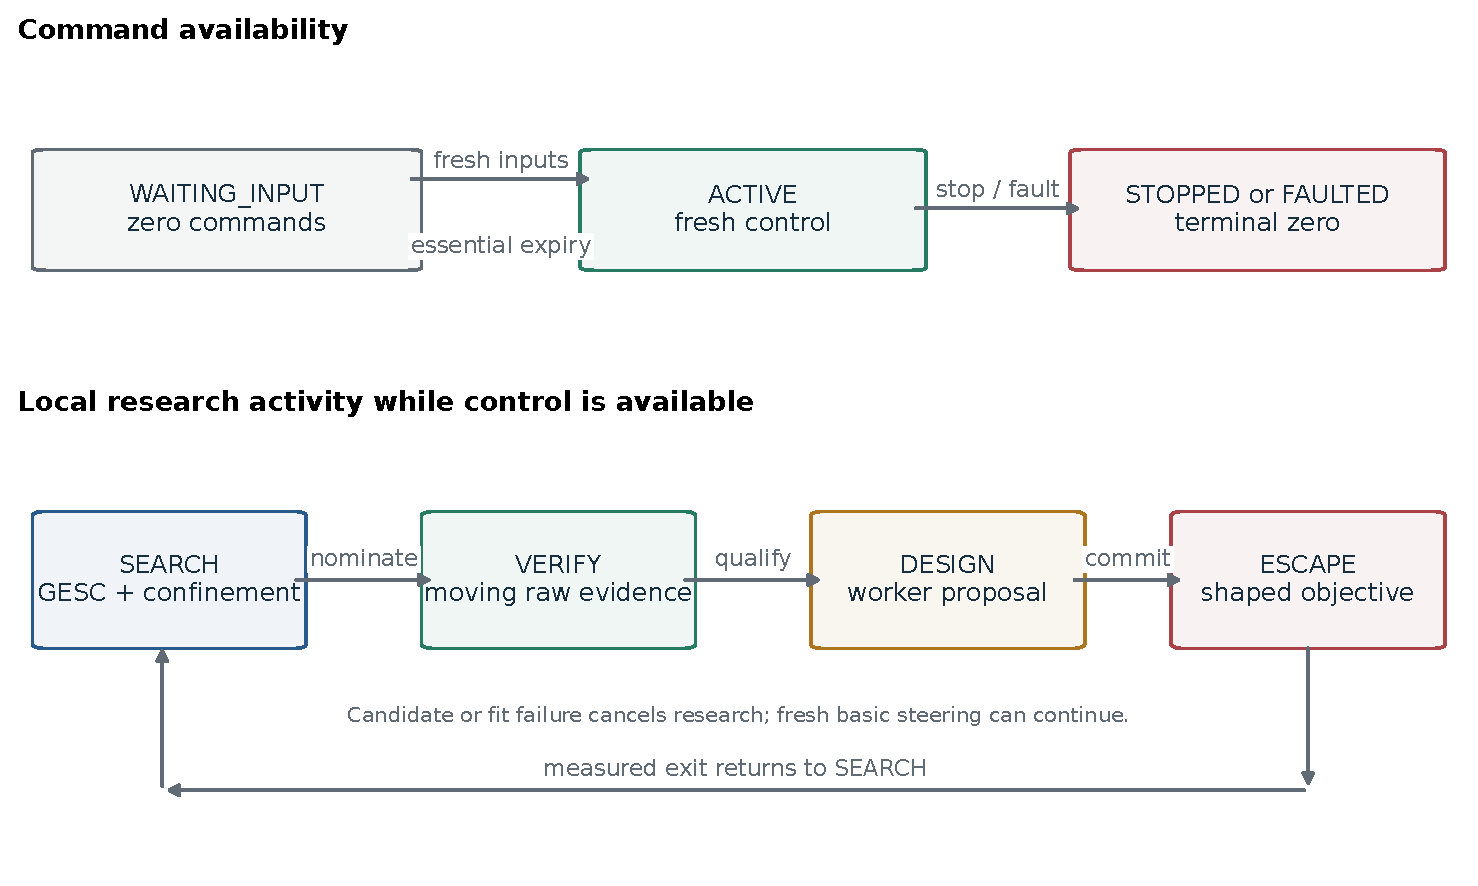
\includegraphics[width=1\linewidth,height=\textheight,keepaspectratio,alt={Command availability and research activity are independent axes.}]{v3/report_figures/state_authority.pdf}
\caption{Command availability and research activity are independent
axes.}
\end{figure}

\subsection{Coordinates, cost sign, and physical
meaning}\label{coordinates-cost-sign-and-physical-meaning}

\subsubsection{Base pose and rotating sensor
pose}\label{base-pose-and-rotating-sensor-pose}

Write the observed base position as \(p_b=(x_b,y_b)\), base yaw as
\(\psi\), arm angle relative to the base as \(\phi\), and arm radius as
\(d\). For the planar geometry used by the selected profile, the sensor
world angle is

\[
\alpha=\psi+\phi,
\]

and the sensor position is conceptually

\[
p_s=p_b+d\begin{bmatrix}\cos\alpha\\\sin\alpha\end{bmatrix},\qquad d=0.18\;\mathrm{m}.
\]

The observation already supplies measured sensor coordinates; the
objective composer uses those coordinates instead of silently
reconstructing a perfect arm. The demodulator uses the body-relative
measured phase \(\phi\). Rolling integration rotates the demodulated
vector using the yaw associated with the observation, then reprojects
the resulting world vector using the current fresh yaw when commanding
the robot.

The fit convention is deliberately different: the basin sample stores
\textbf{base} position and measured raw cost. Thus the fitted data are
\((p_b,J_{\rm raw})\), while objective modification is evaluated at
\(p_s\). This is inherited selected mathematics, not a claim that the
two positions coincide. With a moving base and a directional sensor, a
local fit is an empirical description of these observations. It should
not be mistaken for an exact global map of cost at the sensor.

\emph{Source:
\path|ros2_ws/src/ros_esc/ros_esc/gesc_v3/core.py:203-237|;
\path|ros2_ws/src/ros_esc/ros_esc/gesc_v3/numerics/rolling.py:28-36,264-284,470-520|;
\path|ros2_ws/src/ros_esc/config/profiles/algorithms.json:193-202|;
\path|ros2_ws/src/ros_esc/test/test_v3_core.py:347-352|.}

\begin{figure}
\centering
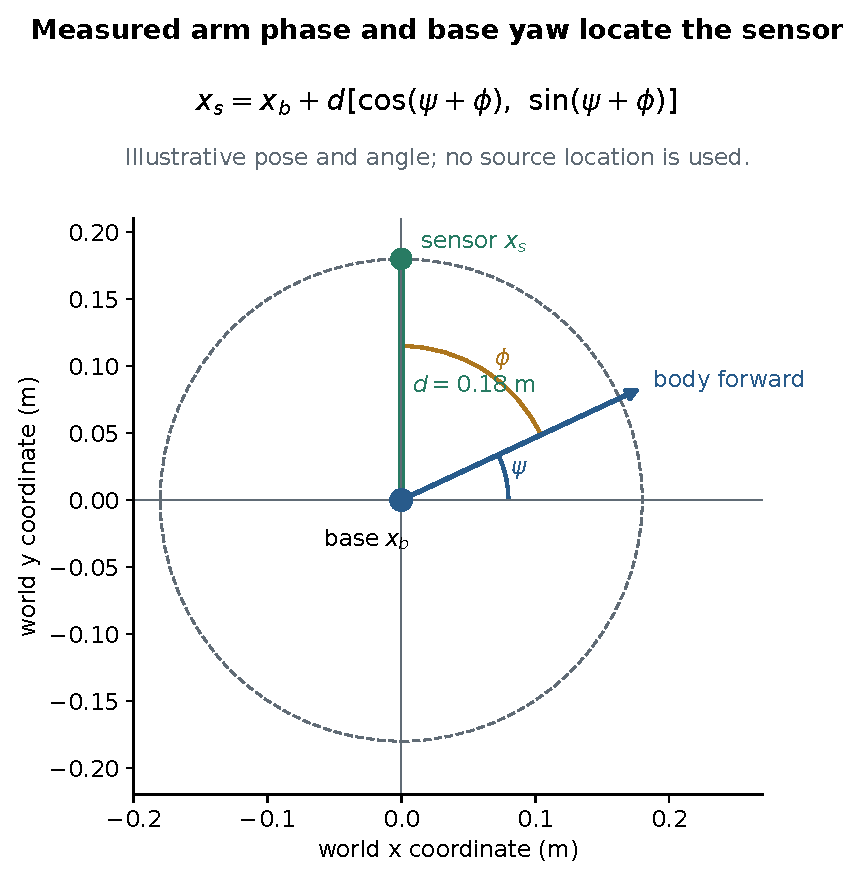
\includegraphics[width=0.9\linewidth,height=\textheight,keepaspectratio,alt={Sensor geometry uses observed yaw and arm phase; source coordinates are absent from control.}]{v3/report_figures/sensor_geometry.pdf}
\caption{Sensor geometry uses observed yaw and arm phase; source
coordinates are absent from control.}
\end{figure}

\subsubsection{Why brighter means a smaller
objective}\label{why-brighter-means-a-smaller-objective}

The selected light model returns a negative divider voltage. If the
positive voltage is \(V\), the minimization cost is

\[
J_{\rm raw}=-V.
\]

A reading of \(+2.8\) V therefore corresponds to \(-2.8\) cost units. It
is better under minimization than \(+1.2\) V, which corresponds to
\(-1.2\). Comparing signed costs as if larger were better reverses the
research objective.

The model's resistance-to-voltage conversion is

\[
J_{\rm raw}=-\frac{5}{R/330+1}.
\]

Here \(R\) is the modeled photoresistor resistance in ohms, and 330 is
the divider resistance in ohms. For \(R=330\;\Omega\), this gives
\(J=-2.5\) V. For \(R=660\;\Omega\), it gives \(J\approx-1.667\) V.
Lower resistance yields higher positive sensor voltage and lower signed
cost.

In the multi-light model, contributions are combined as increments in
conductance, not a sum of output voltages. For source \(j\), its fitted
resistance \(R_j\) depends on distance and sensor bearing; its
nonnegative conductance increment is scaled by its intensity relative to
1000 lumens. The total conductance is dark conductance plus those
contributions, resistance is its reciprocal, and the divider conversion
is applied once. This helps explain why overlapping sources do not
produce a simple sum of two isolated voltage maps.

\emph{Source:
\path|ros2_ws/src/ros_esc/ros_esc/cost_function_node/cost_function_objects/cost_function_objects.py:352-353,457-479,487-527,542-560|;
\path|ros2_ws/src/ros_esc/config/profiles/assets/gesc_v3/cost.json:2-22|.}

\subsubsection{Raw cost, shaped cost, and ranking must stay
separate}\label{raw-cost-shaped-cost-and-ranking-must-stay-separate}

A Gaussian is a positive cost hill. It is added because the controller
minimizes: raising the objective near a previously encountered basin
makes returning there less attractive. An affine term is a directional
slope. These artificial terms are control aids, not stronger light
measurements.

The composer implements

\[
J_{\rm aug}(p_s,t)=w_sJ_{\rm raw}+w_g\sum_iG_i(p_s)+w_aA(p_s,t).
\]

The selected activity weights are:

{\def\LTcaptype{none} % do not increment counter
\begin{longtable}[]{@{}
  >{\raggedright\arraybackslash}p{(\linewidth - 8\tabcolsep) * \real{0.1667}}
  >{\raggedleft\arraybackslash}p{(\linewidth - 8\tabcolsep) * \real{0.2222}}
  >{\raggedleft\arraybackslash}p{(\linewidth - 8\tabcolsep) * \real{0.2222}}
  >{\raggedleft\arraybackslash}p{(\linewidth - 8\tabcolsep) * \real{0.2222}}
  >{\raggedright\arraybackslash}p{(\linewidth - 8\tabcolsep) * \real{0.1667}}@{}}
\toprule\noalign{}
\begin{minipage}[b]{\linewidth}\raggedright
Activity
\end{minipage} & \begin{minipage}[b]{\linewidth}\raggedleft
\(w_s\) raw
\end{minipage} & \begin{minipage}[b]{\linewidth}\raggedleft
\(w_g\) Gaussian
\end{minipage} & \begin{minipage}[b]{\linewidth}\raggedleft
\(w_a\) affine
\end{minipage} & \begin{minipage}[b]{\linewidth}\raggedright
Role
\end{minipage} \\
\midrule\noalign{}
\endhead
\bottomrule\noalign{}
\endlastfoot
SEARCH & 1 & 1 & 0 & Seek using the measured field while discouraging a
filled basin \\
VERIFY & 1 & 1 & 0 & Keep the raw/filled objective available while
moving collection steers \\
DESIGN & 1 & 1 & 0 & Continue moving collection while numerical
preparation runs \\
ESCAPE & 0 & 1 & 1 & Obtain GESC direction from Gaussian plus affine
repulsion \\
\end{longtable}
}

Raw cost remains recorded and is used for candidate quality/ranking
during all activities. It is simply multiplied by zero in the escape
\textbf{control objective}. Calling ESCAPE ``raw plus Gaussian plus
affine'' without specifying these selected weights is incorrect.

A voltage-based raw cost and the Gaussian amplitude have compatible cost
units; covariance has square metres; affine coefficient has cost units
per metre. A shaped objective can be positive even though raw voltage
cost is negative. Its sign alone does not describe source quality. The
normalized model \passthrough{\lstinline!source\_score!} is a separate
quantity and is not what this core uses to rank candidates.

\emph{Source:
\path|ros2_ws/src/ros_esc/ros_esc/gesc_v3/numerics/objective.py:31-50|;
\path|ros2_ws/src/ros_esc/ros_esc/gesc_v3/core.py:203-208,229-237,428-439|;
\path|ros2_ws/src/ros_esc/test/test_v3_core.py:355-370,478-487|.}

\begin{figure}
\centering
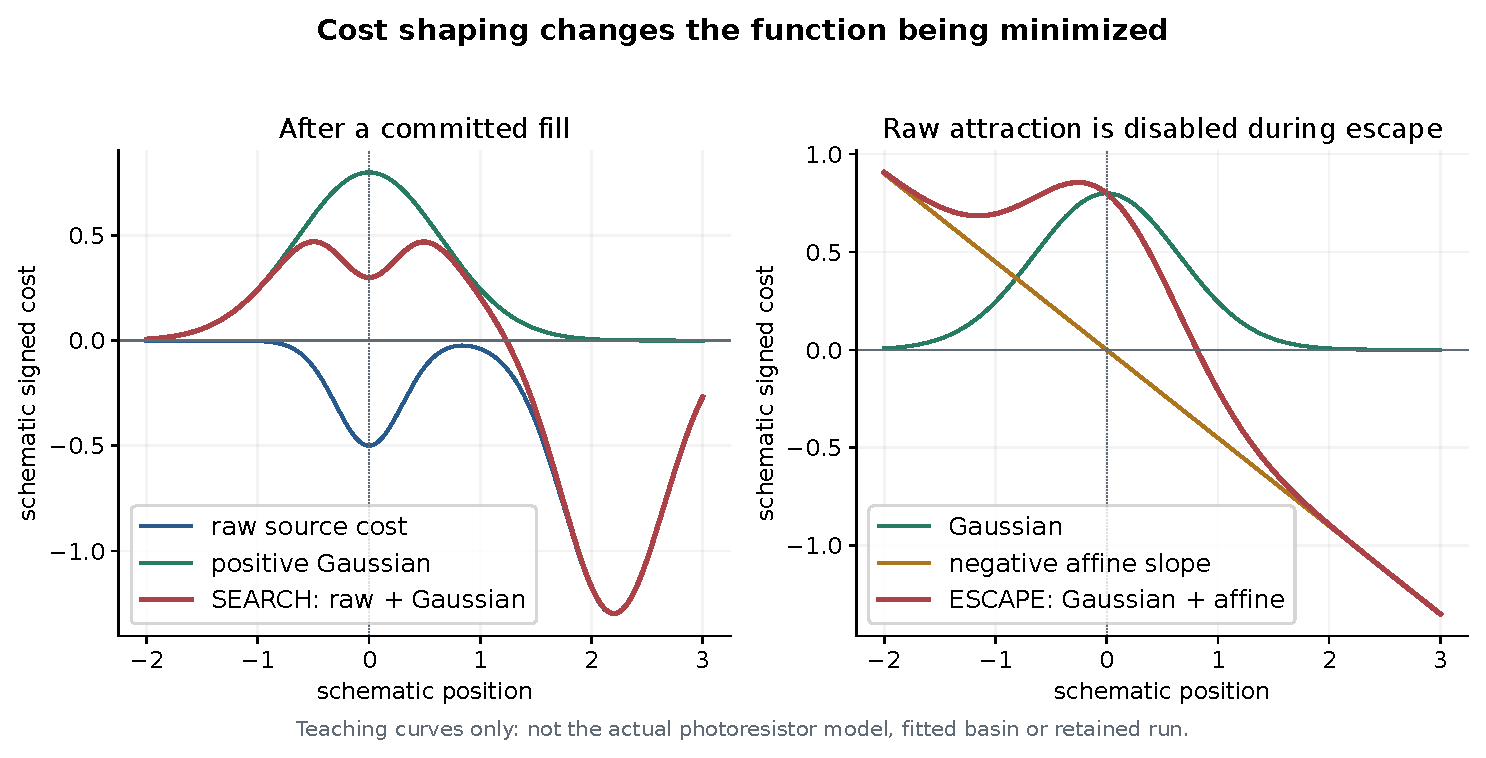
\includegraphics[width=1\linewidth,height=\textheight,keepaspectratio,alt={Schematic objective shaping explains the positive Gaussian and negative affine slope. These curves are teaching examples, not measured field fits.}]{v3/report_figures/objective_shapes.pdf}
\caption{Schematic objective shaping explains the positive Gaussian and
negative affine slope. These curves are teaching examples, not measured
field fits.}
\end{figure}

\subsection{Measured-angle GESC from intuition to
implementation}\label{measured-angle-gesc-from-intuition-to-implementation}

\subsubsection{Why rotating a sensor reveals a
direction}\label{why-rotating-a-sensor-reveals-a-direction}

GESC means gradient extremum-seeking control. It tries to recover a
useful downhill direction from scalar observations instead of receiving
the field gradient directly. A small rotating displacement acts as the
exploratory perturbation.

For intuition, temporarily assume a smooth position-only field, a nearly
fixed base, and a small sensor radius. Let
\(u(\phi)=(\cos\phi,\sin\phi)\). A first-order expansion gives

\[
J(p_b+du)\approx J(p_b)+d\nabla J(p_b)^Tu.
\]

Subtracting the slowly varying baseline leaves approximately
\(d\nabla J^Tu\). Multiplying by \(-(2/d)u\) and averaging an ideal
uniform revolution gives

\[
\left\langle-\frac{2}{d}\,[d\nabla J^Tu]u\right\rangle
=-2\left\langle uu^T\right\rangle\nabla J=-\nabla J,
\]

because the average of \(\cos^2\phi\) and \(\sin^2\phi\) is \(1/2\), and
the average of \(\cos\phi\sin\phi\) is zero. This explains the factor
\(2/d\) and the negative sign.

This is a pedagogical derivation of the chosen demodulation structure.
It is \textbf{not} a proof that every active estimate equals the true
gradient. The implemented light sensor is directional, the base moves,
the washout has dynamics, rotation speed is measured rather than
perfectly uniform, and observations are sparse. V3 preserves the chosen
full-rotation GESC calculation and evaluates it empirically; it does not
replace these facts with the ideal assumptions.

\emph{Source: implemented structure in
\path|ros2_ws/src/ros_esc/ros_esc/gesc_v3/numerics/gesc.py:16-21,37-59|;
directional field dependence in
\path|ros2_ws/src/ros_esc/ros_esc/cost_function_node/cost_function_objects/cost_function_objects.py:487-527|.
The Taylor expansion above is explanatory derivation, not an additional
runtime computation.}

\subsubsection{Washout state and the exact discrete
update}\label{washout-state-and-the-exact-discrete-update}

The scalar state \(z\) tracks the cost baseline:

\[
\dot z=\omega(J_{\rm aug}-z),\qquad\omega=1.0\;\mathrm{s}^{-1}.
\]

The washed signal is \(r=J_{\rm aug}-z\). The instantaneous descent-like
body vector is

\[
q_b=-\frac{2}{d}(J_{\rm aug}-z)\begin{bmatrix}\cos\phi\\\sin\phi\end{bmatrix}.
\]

The implementation computes \(q_b\) using the state \textbf{before} the
Euler update, then performs

\[
z_k^+=z_k^-+\Delta t_k\omega(J_k-z_k^-).
\]

The elapsed time is the difference between actual source timestamps, not
an assumed 0.2 seconds and not the command timer period. The first
observation after a numerical reset has \(\Delta t=0\). Repeated or
decreasing source stamps are invalid. A source gap over 0.5 seconds
resets history rather than inventing observations across the gap.

The magnitude of \(q_b\) is \(2|J-z|/d\). A large absolute cost is not
automatically a large useful direction: it is the cost's difference from
the washout state that supplies the modulation. The direction also
changes sign when \(J-z\) changes sign. Consequently a single sample is
a phase-correlated instantaneous vector, not a complete Cartesian
gradient measurement.

\emph{Source:
\path|ros2_ws/src/ros_esc/ros_esc/gesc_v3/numerics/gesc.py:23-59|;
\path|ros2_ws/src/ros_esc/ros_esc/gesc_v3/records.py:71-80|;
\path|ros2_ws/src/ros_esc/test/test_v3_numerics.py:115-121,261-268|.}

\subsubsection{A worked GESC calculation and startup
priming}\label{a-worked-gesc-calculation-and-startup-priming}

Suppose the core first observes \(J=-2.0\) and initializes \(z=-2.0\).
The first direction is zero: an absolute brightness reading has not yet
supplied a measured change. At the next valid observation, let
\(J=-2.1\), \(\phi=60^\circ\), \(d=0.18\) m, and \(\Delta t=0.2\) s.
Before updating \(z\),

\[
r=-2.1-(-2.0)=-0.1,
\]

\[
q_b=\frac{0.2}{0.18}\begin{bmatrix}0.5\\0.866025\end{bmatrix}
\approx\begin{bmatrix}0.555556\\0.962250\end{bmatrix}.
\]

The derivative is \(\dot z=-0.1\), so \(z^+=-2.02\). The selected
directional controller would request \(v_x=0.5q_x\approx0.2778\) m/s and
\(w_z=5q_y\approx4.8113\) rad/s before saturation; the current Gazebo
caps reduce those requests to 0.10 m/s and 0.50 rad/s.

Priming is a \textbf{core startup} rule. The standalone numerical helper
resets its state to zero and is golden-tested that way. On first core
acquisition, the core explicitly seeds state from the first real
augmented cost so it does not manufacture a direction from the absolute
voltage. After an in-motion objective change, the core resets numerical
history but does \textbf{not} reapply startup priming. The first actual
sample under the new objective is evaluated with that reset state and
zero integration duration. This selected behavior avoids a planned
synthetic transition stop, but also means the transition sample need not
resemble the settled periodic estimate.

\emph{Source:
\path|ros2_ws/src/ros_esc/ros_esc/gesc_v3/core.py:66-69,209-215,272-276|;
\path|ros2_ws/src/ros_esc/ros_esc/gesc_v3/numerics/gesc.py:33-59|;
\path|ros2_ws/src/ros_esc/test/test_v3_core.py:87-109,396-411,618-631|;
controller law in
\path|ros2_ws/src/ros_esc/ros_esc/controller_node/controller_objects/turtlebot_vehicle.py:152-172|.}

\subsubsection{From a direction vector to a differential-drive
command}\label{from-a-direction-vector-to-a-differential-drive-command}

The selected \path|Directional_Controller| uses the simple component
rule

\[
v_x=\operatorname{clip}(k_vq_{b,x},-v_{\max},v_{\max}),\qquad
w_z=\operatorname{clip}(k_wq_{b,y},-w_{\max},w_{\max}).
\]

The selected gains are \(k_v=0.5\), \(k_w=5.0\). The x component
requests signed translation; the y component requests yaw rotation. A
vector pointing behind the robot can request reverse motion. This is not
a controller that must rotate to face the vector before translating. For
\(q_b=(-0.04,0.02)\), the unsaturated command is \((-0.02,0.10)\):
reverse at 2 cm/s while turning positively. For \(q_b=(0,0.2)\),
translation is zero and the angular request saturates. A valid direction
therefore does not guarantee continuous translation.

The numerical API takes a six-state vector
\((x,y,z,\mathrm{roll},\mathrm{pitch},\mathrm{yaw})\) and returns a
six-velocity vector. V3 extracts elements 0 and 5 and clips again to its
selected core caps. In gradient-estimate use, the numerical gain maps
cost-per-metre to velocity; in centered tracking, the same controller
receives a geometric vector. These are tuned numerical mappings, not a
universal physical law giving the same dimensional interpretation to
every upstream vector.

\emph{Source:
\path|ros2_ws/src/ros_esc/ros_esc/controller_node/controller_objects/turtlebot_vehicle.py:117-172|;
\path|ros2_ws/src/ros_esc/ros_esc/gesc_v3/core.py:540-546,562-570|;
\path|ros2_ws/src/ros_esc/config/profiles/assets/gesc_v3/controller.json:4-17|;
\path|ros2_ws/src/ros_esc/test/test_v3_core.py:812-818|.}

\subsection{Rolling direction, actual revolutions, and
coherence}\label{rolling-direction-actual-revolutions-and-coherence}

\subsubsection{Why averaging must occur in a common
frame}\label{why-averaging-must-occur-in-a-common-frame}

A body-frame vector means something different after the robot turns. V3
therefore rotates each sample into the world frame:

\[
q_w(t_i)=R(\psi_i)q_b(t_i),\qquad
R(\psi)=\begin{bmatrix}\cos\psi&-\sin\psi\\\sin\psi&\cos\psi\end{bmatrix}.
\]

For example, a body-forward vector \((1,0)\) observed at yaw
\(90^\circ\) represents world \((0,1)\). Averaging it directly with a
body-forward vector from yaw \(0^\circ\) would erase the distinction
between world north and world east.

The phase used to count revolutions is the measured \textbf{world sensor
phase} \(\alpha=\psi+\phi\). A turn of the base contributes to world
rotation; the arm's nominal motor RPM alone is not the cycle boundary.
Consecutive phases are locally unwrapped by the shortest angular
increment. A step exactly \(\pi\) is ambiguous. Reversal, context
changes, gaps, excessive cycle length, and capacity violations reset
rolling history. There is no free extrapolation of unobserved rotations.

\emph{Source:
\path|ros2_ws/src/ros_esc/ros_esc/gesc_v3/numerics/rolling.py:28-50,252-333|;
\path|ros2_ws/src/ros_esc/ros_esc/gesc_v3/core.py:216-222|.}

\subsubsection{The one-revolution mean is time
weighted}\label{the-one-revolution-mean-is-time-weighted}

At the latest sample time \(t_1\), V3 finds the earlier measured phase
crossing exactly one revolution behind. If a crossing falls between
source samples, it linearly interpolates its time and vector. Between
successive observed vertices the vector is represented linearly. Its
one-revolution mean is

\[
\bar q_w=\frac{1}{T}\sum_j\Delta t_j\frac{q_{w,j}+q_{w,j+1}}{2},\qquad T=t_1-t_0.
\]

This is a temporal trapezoidal mean over a phase-defined window. It is
not simply the arithmetic average of the last 15 observations, and it is
not an angularly uniform integral. Those distinctions matter when arm
speed varies or base yaw changes.

For a toy two-segment window with durations 1 s and 2 s, and endpoint
vectors \((1,0)\), \((3,0)\), \((3,2)\), the mean is
\([(1)(2,0)+(2)(3,1)]/3=(8/3,2/3)\). Equal weighting of its three
vertices would instead give \((7/3,2/3)\). The code uses the former kind
of time accounting.

Three completed anchored cycles, all with valid temporal support,
provide warmup confidence. The current rolling mean still spans the
latest one revolution; it is \textbf{not} the mean of three cycle means.
Each cycle must last no more than 30 seconds and its original source
gaps no more than 0.5 seconds. The selected 5 Hz steering policy records
12 angular sector populations for diagnostics but does not impose a
sector-population gate.

\emph{Source:
\path|ros2_ws/src/ros_esc/ros_esc/gesc_v3/numerics/rolling.py:73-89,308-331,335-401,421-460|;
\path|ros2_ws/src/ros_esc/ros_esc/gesc_v3/numerics/README.md:12-23|.}

\subsubsection{Coherence asks whether vectors reinforce or
cancel}\label{coherence-asks-whether-vectors-reinforce-or-cancel}

A mean can be small because every sample is weak, or because strong
samples point in opposing directions. The selected coherence ratio
distinguishes directional cancellation:

\[
C=\frac{\|\bar q_w\|}{\frac{1}{T}\int_{t_0}^{t_1}\|q_w(t)\|\,dt}.
\]

The numerator is the norm of the temporal vector mean; the denominator
is the temporal mean of the vector norm. The triangle inequality implies
\(0\le C\le1\) for consistent arithmetic. Constant vector \((1,0)\)
gives \(C=1\). Equal-duration \((1,0)\) and \((-1,0)\) contributions can
give a near-zero mean despite large individual magnitudes, so \(C\) is
near zero.

Because \(q_w(t)\) is linearly represented between measurements, the
denominator integrates the \textbf{norm of the interpolated vector}, not
a trapezoid of endpoint norms. A segment from \((1,0)\) to \((-1,0)\)
has average norm \(1/2\) under linear interpolation; averaging the
endpoint norms would give 1. This is why the worker performs bounded
quadrature rather than reusing the numerator's arithmetic.

The code returns an interval, not just a point ratio. If \(D\) is the
denominator, \(\epsilon_D\) its numerical error estimate, and
\(\epsilon_q=\sqrt2\epsilon_{\rm component}\) the numerator tolerance,
it uses

\[
C_{\rm lower}=\frac{\max(0,\|\bar q_w\|-\epsilon_q)}{D+\epsilon_D},
\]

\[
C_{\rm upper}=\min\left(1,\frac{\|\bar q_w\|+\epsilon_q}{D-\epsilon_D}\right).
\]

Qualification requires the lower bound to be at least 0.25, adequate
warmup and coverage, and a mean magnitude above \(10^{-6}\). Error over
\(10^{-10}\), unresolved positive denominator, excessive
triangle-inequality discrepancy, warnings, or exhausted quadrature
budgets make coherence unavailable. These are numerical reconstruction
tolerances; they are not experimentally calibrated uncertainty bounds on
the physical field or source direction.

\emph{Source:
\path|ros2_ws/src/ros_esc/ros_esc/gesc_v3/numerics/coherence.py:14-27,67-157,192-225|;
\path|ros2_ws/src/ros_esc/ros_esc/gesc_v3/numerics/rolling.py:177-197,380-417|.}

\subsubsection{Qualified blending and asynchronous
continuity}\label{qualified-blending-and-asynchronous-continuity}

A qualified mean contributes 75\%; the current instantaneous vector
contributes 25\%:

\[
q_{w,\rm use}=0.25q_{w,\rm instant}+0.75\bar q_w.
\]

An unqualified or unavailable mean contributes zero, so meaningful fresh
instantaneous control remains available. A zero instantaneous sample can
be bridged by a meaningful qualified mixture. A weak or nonfinite
mixture falls back, and a vector below the absolute magnitude floor
cannot drive the controller.

For \(q_{\rm instant}=(1,-1)\) and \(\bar q=(1,0.2)\), a qualified blend
is \((1,-0.1)\). Reprojection at yaw \(90^\circ\) gives body
\((-0.1,-1)\); the current yaw is used even if the vector snapshot was
accepted earlier.

The worker result must exactly match source timestamp, reset sequence,
and objective revision. A result for an old sample cannot give its
confidence to the newest geometry. While a replacement job is pending,
the entire previous accepted snapshot may be held within its original
0.5-second freshness, unchanged frame/objective context and history
sequence. Its original vector and confidence stay together; only its
body projection changes with the fresh yaw. When it expires, the owner
falls back to the newest instantaneous direction. A negative replacement
result revokes the old accepted snapshot.

\emph{Source:
\path|ros2_ws/src/ros_esc/ros_esc/gesc_v3/numerics/rolling.py:403-419,462-520|;
\path|ros2_ws/src/ros_esc/test/test_v3_direction_handoff.py:32-125|;
\path|ros2_ws/src/ros_esc/test/test_v3_core.py:309-331|.}

\subsection{Recognizing recurrence without knowing the
source}\label{recognizing-recurrence-without-knowing-the-source}

\subsubsection{The detector's evidence is trajectory
geometry}\label{the-detectors-evidence-is-trajectory-geometry}

The active mode is \path|recurrent_geometry_v3|. It evaluates observed
base odometry every six source seconds and considers five branches:
static over 30 s, circle over 30 s, circle over 36 s, oscillation over
36 s, and oscillation over 54 s. It preserves source vertices and
interpolates only bracketed support boundaries. The harmonic branch
additionally uses a fixed interpolated time representation for its
finite model search.

It does not read the cost, a source coordinate, or a simulator source
label. Its question is whether the motion looks recurrent and confined.
A stationary robot can satisfy the static geometry; an orbit can satisfy
circle geometry; repeated back-and-forth motion can satisfy harmonic
geometry. Each is a nomination that requires separate raw-cost
verification.

All fits use temporal trapezoidal weights. For support \([t_a,t_b]\),
each source segment contributes half its duration to each endpoint,
normalized by total duration. The time mean is \(\mu=\sum_iw_ip_i\), and
confinement radius is the maximum distance from that mean over supported
vertices. A gap over 0.5 s, frame/time conflict, conflicting duplicate,
or capacity failure resets history.

\emph{Source:
\path|ros2_ws/src/ros_esc/ros_esc/gesc_v3/numerics/recurrent.py:14-15,51-75,115-128,162-167,216-341|;
\path|ros2_ws/src/ros_esc/ros_esc/gesc_v3/core.py:145-153|;
\path|ros2_ws/src/ros_esc/test/test_v3_core.py:908-925,962-970|.}

\subsubsection{Static and circular
recurrence}\label{static-and-circular-recurrence}

For the static branch, the detector fits a constant plus linear drift to
centered x/y motion. The drift norm must be at most 0.005 m/s and every
supported vertex within 0.04 m of the mean. One eligible complete
30-second evaluation is enough to confirm this branch. ``Static'' is a
geometric label; it does not authorize stationary verification.

For each circle branch, the support is split into equal older/newer
halves. Each half is fit to a circle by weighted algebraic least
squares. With centered coordinates \(r_i=p_i-o\), the design fits

\[
2r_{i,x}c_x+2r_{i,y}c_y+a=\|r_i\|^2,
\]

then returns center \(o+c\), radius \(\sqrt{a+\|c\|^2}\), weighted
radial RMS residual, and net unwrapped bearing change. Rank must be
three and radius square positive.

A circle branch passes only when the entire support is confined within
0.5 m of its time mean, center drift between halves is at most 0.006
m/s, the two fitted radii differ by at most 0.08 m, and each half has
radius 0.03-0.5 m, radial RMS at most 0.02 m, and at least \(\pi/3\) net
bearing change. Circle branches require three consecutive eligible
evaluations, six seconds apart. A 30-second branch can therefore first
confirm at approximately 42 seconds after complete fresh support begins,
subject to evaluation alignment.

As a calculation, two half-circle centers 0.03 m apart over a 15-second
half support give drift \(0.03/15=0.002\) m/s, which meets the drift
gate. That alone is insufficient: poor residuals, a radius change,
insufficient arc, or excessive global confinement can still reject the
candidate. The detector checks a conjunction of evidence, not a single
score threshold.

\emph{Source:
\path|ros2_ws/src/ros_esc/ros_esc/gesc_v3/numerics/recurrent.py:131-146,162-191,303-337|.}

\subsubsection{Harmonic oscillation and
persistence}\label{harmonic-oscillation-and-persistence}

The oscillation branch first checks line-like geometry. A weighted
planar covariance has eigenvalues \(\lambda_1\le\lambda_2\).
Perpendicular RMS is \(\sqrt{\lambda_1}\) and axis-variance ratio is
\(\lambda_1/\lambda_2\). The support must remain within 0.5 m,
perpendicular RMS at most 0.02 m, and ratio at most 0.1.

It then fits both coordinates to

\[
p(t)\approx a+b\frac{t}{W}+c\cos(2\pi t/P)+s\sin(2\pi t/P),
\]

using an interpolated 0.2-second grid centered in a support of width
\(W\). Candidate periods range from 6 s to \(\min(96,W/0.75)\) s in
0.5-second steps. The smallest weighted squared residual chooses the
period. The fitted drift norm is \(\|b\|/W\); the amplitude is the
largest singular value of the two-dimensional sine/cosine coefficient
matrix.

Acceptance requires drift at most 0.006 m/s, amplitude at least 0.05 m,
weighted residual RMS at most 0.02 m, and weighted design condition
number at most 50. Three consecutive passes are required. The
corresponding earliest complete-support confirmations are about 48 s for
the 36-second branch and 66 s for the 54-second branch, with timing
subject to the epoch evaluation schedule.

The reported score is drift multiplied by 12 s, producing metres. For
static, its maximum drift corresponds to 0.060 m; for circle/harmonic it
corresponds to 0.072 m. The score is telemetry summarizing one
condition. Replacing the branch predicates by ``score below 0.072''
would discard radius, shape, residual, amplitude, condition and
persistence gates. Nor is this the historical two-block centroid
detector, despite inherited \passthrough{\lstinline!CentroidResult!}
field names.

\emph{Source:
\path|ros2_ws/src/ros_esc/ros_esc/gesc_v3/numerics/recurrent.py:14-15,17-47,149-159,192-213,303-337|;
golden model cases in
\path|ros2_ws/src/ros_esc/test/test_v3_numerics.py:89-107,137-138|.}

\subsection{Moving verification and three-cycle raw
evidence}\label{moving-verification-and-three-cycle-raw-evidence}

\subsubsection{Approaching a fixed candidate and circling
it}\label{approaching-a-fixed-candidate-and-circling-it}

A recurrent nomination freezes a candidate center \(c\). VERIFY keeps
the base within a 0.75 m candidate neighborhood. It first approaches
that center using world vector \(c-p_b\). When base distance reaches
0.08 m, collection is marked started. It then uses a tiny circular
reference

\[
p_d=c+0.03\begin{bmatrix}\cos(0.3\tau)\\\sin(0.3\tau)\end{bmatrix},\qquad
\dot p_d=0.009\begin{bmatrix}-\sin(0.3\tau)\\\cos(0.3\tau)\end{bmatrix},
\]

where \(\tau\) is elapsed time since the \textbf{candidate start},
including approach. The world tracking input is

\[
q_{\rm track}=p_d-p_b+\dot p_d/0.5.
\]

It is rotated into the body frame and passed to the same directional
controller. Under a simplified point-integrator interpretation, a
proportional gain 0.5 times this input would supply proportional error
correction plus desired reference velocity. The actual
differential-drive law and saturation mean exact circle tracking is not
guaranteed.

The reference circle radius is 3 cm, angular rate 0.3 rad/s, period
about 20.94 s, and tangent speed 0.009 m/s. It is a \textbf{base motion
reference}, distinct from the sensor's nominal 20 RPM rotation, whose
period is approximately 3 seconds. Entering the 8 cm collection radius
does not restart the reference phase.

Valid moving approach and collection have no elapsed deadline. However,
measured translation below 1 mm over a 0.5-second check interval cancels
the research candidate. DESIGN inherits that moving requirement and has
its separate finite preparation budget. ``No candidate deadline''
therefore means continue gathering valid moving evidence, not ignore
stale inputs or accept a stopped base.

\emph{Source:
\path|ros2_ws/src/ros_esc/ros_esc/gesc_v3/numerics/verification.py:5-20|;
\path|ros2_ws/src/ros_esc/ros_esc/gesc_v3/core.py:242-252,401-427,488-507,548-560|;
\path|ros2_ws/src/ros_esc/test/test_v3_core.py:202-264,890-905|.}

\subsubsection{Steering coverage and verification coverage are
different}\label{steering-coverage-and-verification-coverage-are-different}

Moving raw evidence counts actual complete sensor-world revolutions. Its
cycle boundaries are phase crossings interpolated between actual
observations. Each cycle must have at least one actual raw sample in
each of 12 angular sectors and positive represented time in each sector.
Interpolation can establish a boundary or geometric support; it cannot
populate an empty cost sector with a fabricated acquisition.

The owner selects the latest three \textbf{eligible} cycles. Each cycle
must be qualified, all measured/interpolated trajectory vertices lie
within 0.75 m of the candidate, and its time centroid within 0.15 m of
the center. For every sector, time-weighted base position centroids
across the three cycles must differ by no more than 0.15 m. This sector
comparability prevents treating measurements taken from substantially
different base paths as equivalent rotations. Snapshot support,
including real samples bracketing boundaries, must remain available and
at most 4000 samples.

At ideal 5 Hz and 20 RPM, there are 15 samples per nominal revolution
and a 24-degree nominal angular step. Twelve sectors span 30 degrees
each, so coverage is possible but sensitive to actual phase, yaw motion,
missing samples and varying speed. ``Three cycles exist'' is not
equivalent to ``three qualified comparable cycles exist.'' The rolling
steering policy can meanwhile use instantaneous fallback because its
selected coverage does not require all sectors populated.

Pretrigger cycles are permitted: a selected cycle ending before the
detector confirmation is counted as pretrigger, with later cycles
counted as verification evidence. VERIFY does not blindly demand three
brand-new revolutions after entering the center radius. This helps reuse
genuine recent raw support but makes correct epoch and support
accounting important.

\emph{Source:
\path|ros2_ws/src/ros_esc/ros_esc/gesc_v3/numerics/evidence.py:172-183,260-299,304-374,386-423|;
\path|ros2_ws/src/ros_esc/ros_esc/gesc_v3/core.py:424-439|; compare
\path|ros2_ws/src/ros_esc/ros_esc/gesc_v3/numerics/rolling.py:371-378|.}

\subsubsection{The candidate cost interval and the informative
diagnostic}\label{the-candidate-cost-interval-and-the-informative-diagnostic}

Each selected cycle contributes its minimum actual raw cost. For three
minima \(m_1,m_2,m_3\), the estimate is their median, the median
absolute deviation is MAD, and the uncertainty is \(3\,\mathrm{MAD}\):

\[
\widehat J=\operatorname{median}(m_i),\qquad
\mathrm{MAD}=\operatorname{median}(|m_i-\widehat J|),\qquad
I=[\widehat J-3\mathrm{MAD},\widehat J+3\mathrm{MAD}].
\]

For minima \((-2.10,-2.00,-2.05)\), \(\widehat J=-2.05\), MAD is 0.05
and the interval is \([-2.20,-1.90]\). It summarizes rotation
repeatability robustly; it is not a statistical confidence interval with
a claimed coverage probability.

The evidence module also computes zero-mean sector cost profiles, their
average profile RMS amplitude, and pairwise RMS disagreement. A stricter
diagnostic \passthrough{\lstinline!informative!} requires amplitude
greater than three times disagreement or the numerical floor, whichever
is greater. The selected \path|recurrent_trapping_v1| readiness policy
\textbf{does not require that informative flag}. It requires valid
finite summaries, a negative median sector baseline and a negative upper
cost bound beyond a floor \(\max(10^{-6},64\max\mathrm{ulp}(J))\). The
recurrent geometric nomination supplies the trapping rationale
separately. This distinction is easy to lose when reading the earlier
computation above the selected readiness branch.

The algorithm never substitutes the Gaussian-shaped objective for these
minima. Otherwise the robot could rank its own artificial hill as if it
were source evidence.

\emph{Source:
\path|ros2_ws/src/ros_esc/ros_esc/gesc_v3/numerics/evidence.py:15-103,419-454|;
\path|ros2_ws/src/ros_esc/ros_esc/gesc_v3/core.py:229-237,424-439|;
\path|ros2_ws/src/ros_esc/test/test_v3_numerics.py:141-147|.}

\subsection{Estimating the basin from immutable
observations}\label{estimating-the-basin-from-immutable-observations}

\subsubsection{What data enter the fit, and what is
rejected}\label{what-data-enter-the-fit-and-what-is-rejected}

The worker receives the verified snapshot, a detached registry snapshot
and finite numerical settings. The active core requests a minimum of 20
valid samples; this overrides the estimator class's generic default of
40. The core's immutable support spans the verified rotations, so
\path|freeze_sample_window| is called with explicit snapshot bounds. Its
generic 8-second fitting window and 12-second maximum age are not
allowed to trim that selected rotation support silently.

Filtering rejects nonfinite coordinates/yaw/raw cost, nonpositive
algorithm state, nonincreasing timestamps and position jumps greater
than 0.20 m/s times the actual sample interval. It then applies modified
MAD z scores to raw costs and successive position increments. The
formula is

\[
z_i^{\rm MAD}=0.67448975\frac{|v_i-\operatorname{median}(v)|}{\max(\mathrm{MAD}(v),s_{\rm floor})}.
\]

Values over 3.5 are rejected. Raw-cost scoring has no explicit
denominator floor beyond machine precision handling; position-increment
scoring uses \(10^{-4}\) m as a floor to avoid near-zero numerical MAD
rejecting encoder-scale alternation. The absolute speed-jump gate
remains independent. If the MAD scale is effectively zero, the routine
returns zero scores rather than dividing by zero.

These filters are not a proof that all remaining sensor readings are
accurate. They define which synchronized selected observations the
robust fit will use. A failed minimum count cancels preparation without
stopping otherwise fresh GESC or consuming a fill identity.

\emph{Source:
\path|ros2_ws/src/ros_esc/ros_esc/gesc_v3/core.py:433-439|;
\path|ros2_ws/src/ros_esc/ros_esc/gesc_v3/numerics/basin.py:24-45,123-224|;
\path|ros2_ws/src/ros_esc/ros_esc/gesc_v3/numerics/fill.py:53-101|.}

\subsubsection{Low-cost spatial mean
shift}\label{low-cost-spatial-mean-shift}

The estimator normalizes cost relative to the smallest sample and its
90th-percentile span:

\[
\widetilde J_i=\operatorname{clip}\left(\frac{J_i-J_{\min}}{\max(P_{90}(J)-J_{\min},10^{-12})},0,1\right).
\]

Starting at the position with lowest raw cost, it forms normalized
weights

\[
w_i\propto\exp\left[-\frac{\|p_i-c\|^2}{2h^2}-\frac{\widetilde J_i}{T_J}\right],\qquad
h=0.25\;\mathrm{m},\quad T_J=0.05,
\]

then replaces \(c\) by \(\sum_iw_ip_i\). It performs at most five
iterations and can stop when the center moves less than 5 mm.
Normalization subtracts the maximum log weight before exponentiation so
tiny absolute weights do not underflow together.

The first exponent favors nearby positions; the second favors low signed
cost. With otherwise equal geometry, a sample of normalized cost 0 has
weight \(e^{10}\approx22026\) times a sample of normalized cost 0.5.
This is strong preference for the best observed cost, tempered by
spatial locality and finite iterations. The result is a robust weighted
center, not a Newton step or a solve of \(\nabla J=0\).

\emph{Source:
\path|ros2_ws/src/ros_esc/ros_esc/gesc_v3/numerics/basin.py:227-253,363-396|.}

\subsubsection{Covariance and Hessian describe different
things}\label{covariance-and-hessian-describe-different-things}

The weighted sample covariance is

\[
C_p=\sum_iw_i(p_i-c)(p_i-c)^T.
\]

It has units m\(^2\) and describes where useful samples were
distributed. Its eigenvalues are clipped to \([0.0025,0.25]\) m\(^2\),
corresponding to sample standard deviations between 0.05 and 0.5 m.

Separately, a weighted regularized quadratic is fit:

\[
\widehat J(p)=a+g^T\delta+\tfrac12\delta^TH\delta,\qquad\delta=p-c.
\]

The six design columns are
\(1,\delta_x,\delta_y,\delta_x^2/2,\delta_x\delta_y,\delta_y^2/2\).
Weighted normal equations use ridge \(10^{-6}\) on all coefficients
except the intercept. A finite predictor can be retained even when full
fit validity fails; full validity requires rank at least six and
condition number at most \(10^8\). The symmetric Hessian \(H\) has cost
units per m\(^2\). Its positive-eigenvalue part \(H_+\) is used for
curvature-based amplitude sizing; negative fitted curvature is not
interpreted as a basin stiffness to overcome.

For example, \(C_p=\operatorname{diag}(0.01,0.0025)\) says low-cost
sample spread is 0.10 m along x and 0.05 m along y. A Hessian
\(H=\operatorname{diag}(4,8)\) instead says the fitted cost rises
quadratically with greater curvature along y. These matrices may have
different eigenvectors and should not be called interchangeable ``shape
matrices.'' The fill uses sample covariance for width and positive
Hessian for amplitude rationale.

\emph{Source:
\path|ros2_ws/src/ros_esc/ros_esc/gesc_v3/numerics/basin.py:256-277,294-360,397-402|;
\path|ros2_ws/src/ros_esc/ros_esc/gesc_v3/numerics/fill_design.py:185-208|.}

\subsubsection{Depth and coverage
diagnostics}\label{depth-and-coverage-diagnostics}

Center cost is a weighted 10th percentile of raw costs. Samples outside
Mahalanobis radius one under the clipped sample covariance supply the
shoulder pool; if none exist, all samples become the explicit fallback
pool. Shoulder cost is its 80th percentile, and basin depth is

\[
D_b=\max(J_{\rm shoulder}-J_{\rm center},0.02).
\]

Depth is positive cost difference under minimization. A center at
\(-2.4\) and shoulder at \(-1.8\) give depth 0.6, not \(-0.6\). The
floor prevents a zero-depth proposal from receiving no fill rationale.

Angular coverage is the fraction of eight geometric base-position bins
represented around the fitted center. Spatial coverage is the major
sample standard deviation divided by 0.25 m, capped at one. These are
fit confidence diagnostics. They are different from the twelve
\textbf{sensor phase} sectors used for raw-cycle evidence. A nearly
stationary base can have sensor-phase coverage while poor geometric
spread makes a quadratic poorly conditioned.

\emph{Source:
\path|ros2_ws/src/ros_esc/ros_esc/gesc_v3/numerics/basin.py:280-291,403-435|.}

\subsection{Designing and storing the positive Gaussian
hill}\label{designing-and-storing-the-positive-gaussian-hill}

\subsubsection{Gaussian equation and its downhill
effect}\label{gaussian-equation-and-its-downhill-effect}

A fill with center \(c\), amplitude \(A>0\) and symmetric
positive-definite covariance \(\Sigma\) is

\[
G(p)=A\exp\left[-\tfrac12(p-c)^T\Sigma^{-1}(p-c)\right].
\]

Its gradient is

\[
\nabla G(p)=-G(p)\Sigma^{-1}(p-c),
\]

so descent \(-\nabla G\) points away from the center. At the center the
gradient is zero; a symmetric Gaussian alone does not choose an exit
direction there. This motivates retaining an affine directional slope
during escape.

For isotropic \(\Sigma=0.25I\) m\(^2\) and \(A=2\) cost units, a point
0.5 m from the center has \(G=2e^{-1/2}\approx1.2131\). At
\((c_x+0.5,c_y)\), \(\nabla G\approx(-2.4261,0)\) cost units/m, and
downhill points in positive x. Along a major axis at \(2.7\sigma\),
Gaussian value is \(Ae^{-2.7^2/2}\approx0.0261A\). The chosen exit
radius is a practical geometric threshold, not the point where the
Gaussian mathematically becomes zero. Gaussian tails remain outside the
displayed support radius.

\emph{Source:
\path|ros2_ws/src/ros_esc/ros_esc/gesc_v3/numerics/fill_design.py:138-170,230-245|;
\path|ros2_ws/src/ros_esc/ros_esc/gesc_v3/numerics/registry.py:326-344|.}

\subsubsection{Width and amplitude
selection}\label{width-and-amplitude-selection}

The initial fill covariance is

\[
\Sigma_0=2.5C_p+\sigma_{\rm floor}^2I,
\]

with principal widths clipped between selected floor 0.5 m and ceiling
1.25 m. The current core overrides the generic designer floor 0.15 m. It
also selects amplitude cap 6.25 and exit multiplier 2.7 rather than the
generic defaults 3.0 and 2.5.

Using the covariance example above, selected initial eigenvalues are
\((0.275,0.25625)\) m\(^2\), so widths are approximately
\((0.5244,0.5062)\) m. The geometric covariance floor is not simply
``set both widths to exactly 0.5 m'': the retained sample spread is
added before clipping.

Amplitude must satisfy several proposed floors:

\[
A_{\rm depth}=1.5D_b,
\]

\[
A_{\rm curvature}=1.2\lambda_{\max}(H_+)\lambda_{\max}(\Sigma),
\]

\[
A_{\rm candidate}=\min(1.25[-J_{\rm lower}],6.25),
\]

and

\[
A_0=\operatorname{clip}\bigl(\max(0.10,A_{\rm depth},A_{\rm curvature},A_{\rm candidate}),0.10,6.25\bigr).
\]

The lower raw interval is conservative for a negative cost: multiplying
its magnitude raises the hill enough to account for a stronger plausible
candidate. With \(J_{\rm lower}=-2.20\), this floor is 2.75. If depth is
0.6, its floor is 0.9. If maximum positive curvature is 8 and covariance
major eigenvalue 0.275, curvature floor is \(1.2(8)(0.275)=2.64\).
Candidate-informed amplitude therefore selects at least 2.75 before
validation in this example.

Curvature scaling follows the local Hessian effect of a Gaussian. At its
center, \(\nabla^2G=-A\Sigma^{-1}\), so adding a positive hill supplies
negative curvature against a positive-curvature well. Broadening a
fixed-amplitude hill weakens its center curvature; width and amplitude
must therefore be coupled. The implementation's maximum-eigenvalue rule
is a conservative sizing heuristic followed by numerical grid
validation, not a universal analytic guarantee on the actual field.

\emph{Source:
\path|ros2_ws/src/ros_esc/ros_esc/gesc_v3/core.py:433-439|;
\path|ros2_ws/src/ros_esc/ros_esc/gesc_v3/numerics/fill_design.py:13-31,102-122,174-228|.}

\subsubsection{What fill validation
establishes}\label{what-fill-validation-establishes}

The designer evaluates fitted quadratic plus Gaussian on a 41-by-41 grid
spanning \(\pm3\) Gaussian widths in each principal coordinate. It
counts interior eight-neighbor minima within selected Mahalanobis exit
support 2.7. A grid point counts as a minimum when it is no greater than
all neighbors within tolerance \(10^{-9}\) and strictly lower than at
least one neighbor beyond that tolerance.

If residual minima remain, at most five escalation rounds are allowed.
Each round first increases amplitude by factor 1.5 up to 6.25 and
retests. If needed, widths increase by factor 1.25 up to 1.25 m and
amplitude is also increased by \(1.25^2\) up to its cap, then the grid
is retested. Width expansion changes covariance and derived radii.
Preparation succeeds only when the residual fitted grid-minimum count is
zero. Failure retains no partially committed fill.

This establishes a bounded property of the \textbf{fitted model on that
finite grid}. It is not a proof that the real light field has no minima,
a proof of global convergence, or a trajectory guarantee. An
invalid/ill-conditioned quadratic still contributes a finite predictor
where possible, while fit confidence reflects that limitation; the core
does not impose a hidden ``confidence above 0.6'' admission gate.

The reported confidence averages six clipped components: sample count,
angular/spatial coverage, conditioning, relative residual, cap usage and
grid success. It is descriptive quality evidence, not a probability of
successful escape. Although the generic designer has a low-confidence
threshold 0.60 field, active preparation only requires design success,
and no runtime branch checks that threshold.

\emph{Source:
\path|ros2_ws/src/ros_esc/ros_esc/gesc_v3/numerics/fill_design.py:260-426|;
\path|ros2_ws/src/ros_esc/ros_esc/gesc_v3/numerics/fill.py:122-144|;
\path|ros2_ws/src/ros_esc/ros_esc/gesc_v3/numerics/basin.py:314-359|.}

\subsubsection{The registry prevents double counting and stale
commits}\label{the-registry-prevents-double-counting-and-stale-commits}

Each fill has a fill ID, cluster ID and revision. The registry retains
immutable versions; only the newest active version of each cluster
contributes to objective value. A revision supersedes its old fill
rather than adding both hills on top of one another. Gaussian arrays are
copied and made read-only.

Generic association gives each cluster a normalized score proportional
to \(\exp[-\|c-c_i\|^2/(2h_m^2)]\), with \(h_m=0.5\) m. A merge requires
probability at least 0.6 \textbf{and} distance no more than twice the
greater candidate/current major width. With a single cluster, its
normalized probability is one even for a distant point; the hard
distance gate is therefore essential. This is a relative association
score, not a calibrated probability that two real sources are identical.

Preparation allocates no ID. The main owner stages a complete commit,
verifies the expected registry generation and exact target revision,
validates finite positive geometry and strictly ordered retained
support, and only then commits atomically. Invalid or stale work changes
neither registry generation nor next ID. Runtime strict mode refuses
support conflicts and decimation. Generic legacy registry convenience
routines can evenly decimate oversized history, but active preparation
explicitly caps and rejects a merged snapshot over 4000 rather than
quietly using that route.

In the selected active core there is only one fill. Once a fill exists,
later verified candidates are ranked instead of sent to new fill
preparation. Registry merge/revision functionality remains supported
pure machinery, but it should not be described as a regularly exercised
multi-fill runtime policy in this profile.

\emph{Source:
\path|ros2_ws/src/ros_esc/ros_esc/gesc_v3/numerics/registry.py:12-29,33-64,106-175,266-344|;
\path|ros2_ws/src/ros_esc/ros_esc/gesc_v3/numerics/fill.py:67-144|;
\path|ros2_ws/src/ros_esc/ros_esc/gesc_v3/core.py:347-366,428-439|;
\path|ros2_ws/src/ros_esc/test/test_v3_core.py:415-459|.}

\subsection{Escape direction, affine guidance, and measured
completion}\label{escape-direction-affine-guidance-and-measured-completion}

\subsubsection{The direction continues the approach through the
basin}\label{the-direction-continues-the-approach-through-the-basin}

After fill commitment, the core obtains a direction from observed pose
history. It looks for the newest pose strictly outside the new fill's
frozen escape radius and points from that anchor \textbf{toward the fill
center}. Continuing that vector carries the robot through and out of the
basin on the opposite side. It does not reverse the approach by default.

If no outside anchor exists, the active core enables the helper's
interior fallback: select the farthest retained pose only if its
displacement from the center is at least 0.5 m. If neither anchor can
justify a direction, escape research is cancelled. A committed fill
remains registry data; failed direction selection does not rewrite it.

The unit direction is latched using the direct open-field selector. In
the active core the other-fill list is empty and no room bounds are
supplied. The selector is not reading wall positions or choosing a path
to a known best source. The \passthrough{\lstinline!recent\_approach!}
displacement over 0.5 s is retained in frozen escape geometry, but the
actual latched direction comes from the longer approach-continuity
anchor described above.

For center \((1,1)\) and newest outside anchor \((0,1)\), the direction
is \((1,0)\), not \((-1,0)\). If all history is interior and the
farthest position is \((0.4,1)\), its 0.6 m displacement may qualify the
enabled fallback, again producing \((1,0)\). An anchor only 0.2 m away
cannot supply that fallback.

\emph{Source:
\path|ros2_ws/src/ros_esc/ros_esc/gesc_v3/core.py:368-399|;
\path|ros2_ws/src/ros_esc/ros_esc/gesc_v3/numerics/escape.py:260-388,502-546,623-653|.}

\subsubsection{The affine field chooses a
side}\label{the-affine-field-chooses-a-side}

For unit escape direction \(u_e\), selected affine magnitude
\(\beta=2.0\) and fill anchor \(c\), the core creates \(b_0=\beta u_e\).
The affine value is

\[
A(p,t)=-e^{-\lambda(t-t_e)}b_0^T(p-c),\qquad\lambda=5\times10^{-7}\;\mathrm{s}^{-1},
\]

using age clamped at zero for evaluation before creation. Its gradient
is \(-e^{-\lambda\Delta t}b_0\), so descent points along \(u_e\). If
\(u_e=(1,0)\), a point 0.4 m to the right has affine value approximately
\(-0.8\), and a point 0.4 m to the left has \(+0.8\). Lower cost favors
continuing right. The Gaussian provides outward repulsion; the affine
term breaks directional symmetry and biases which side to leave.

The standalone \passthrough{\lstinline!AffineTerm!} default maximum age
is 30 seconds, but active escape passes
\passthrough{\lstinline!maximum\_age\_sec=0!}, disabling that cutoff.
There is also no elapsed escape-attempt deadline. The term is removed
when escape completion/cancellation actually changes the objective, or
terminal stop/fault cancels it. At 60 seconds its decay multiplier is
\(e^{-0.00003}\approx0.999970\), so the selected exponential changes
very slowly. Calling it a rapidly fading kick is misleading. Its norm
floor is \(10^{-4}\); under ordinary trial durations it remains
essentially its selected slope.

An affine slope is still applied through the measured-angle GESC
washout/demodulation pipeline. It is not a direct velocity command.
Increasing magnitude can change cost modulation and unsaturated
steering, but the same velocity caps still apply. It does not enable the
separate direct assistance option.

\emph{Source:
\path|ros2_ws/src/ros_esc/ros_esc/gesc_v3/numerics/objective.py:8-28|;
\path|ros2_ws/src/ros_esc/ros_esc/gesc_v3/core.py:383-399|;
\path|ros2_ws/src/ros_esc/config/profiles/assets/gesc_v3/controller.json:14-17|;
\path|ros2_ws/src/ros_esc/test/test_v3_core.py:504-527,564-609|.}

\subsubsection{Spatial exit uses two separate time
windows}\label{spatial-exit-uses-two-separate-time-windows}

The frozen escape center and exit radius define radial distance
\(r(t)=\|p_b(t)-c\|\). The ordinary progress tracker compares it to an
interpolated radial distance exactly three seconds earlier:

\[
\Delta r_3(t)=r(t)-r(t-3\;\mathrm{s}).
\]

Exit qualification requires \(r>r_{\rm exit}\), a fully observed
progress window and \(\Delta r_3\ge0\). These conditions must then hold
for \textbf{one second} to establish stable exit. Thus the
implementation has a three-second progress window and a one-second exit
hold; it does not require ``three seconds continuously outside'' as a
single hold condition. The exit radius is \(2.7\sigma_{\rm major}\) in
selected fill design, a conservative circular envelope based on the
widest Gaussian axis.

A tracker also calls progress stalled when the full window exists, exit
is not qualified, and outward radial gain is below 0.05 m. Stalling does
not end escape automatically. With direct assistance disabled, fresh
Gaussian-plus-affine GESC keeps operating until measured exit,
interruption or terminal stop/fault.

When stable exit is seen on a command tick, the core marks a pending
return to SEARCH but keeps the current objective briefly. The next
actual valid source observation removes affine guidance and resets
objective history. It then evaluates the new objective on that real
observation. An old direction is not relabeled as a sample of the new
objective, and history is not replayed. The continuation is still
bounded by essential input freshness.

\emph{Source:
\path|ros2_ws/src/ros_esc/ros_esc/gesc_v3/numerics/escape.py:391-499|;
\path|ros2_ws/src/ros_esc/ros_esc/gesc_v3/core.py:190-208,254-276,508-538|;
\path|ros2_ws/src/ros_esc/test/test_v3_core.py:564-643|.}

\subsubsection{Direct assistance is available but currently
off}\label{direct-assistance-is-available-but-currently-off}

The current selected JSON has
\path|direct_escape_assistance_enabled: false|. This allows the
experiment to study escape through the shaped GESC objective. The
optional fallback remains implemented: a separate tracker uses a
15-second observed radial-progress window. If gain is below 5 cm, exit
is unqualified and assistance has not already been consumed, it triggers
one pulse along the latched world direction.

The pulse uses the \textbf{normal signed directional controller} after
rotating the unit direction into the current body frame. It ends when
newly accepted odometry increments sum to 0.20 m of measured path. This
is path length, not net outward displacement. Forward 8 cm, reverse 8 cm
and forward 4 cm consume 20 cm while leaving only 4 cm net displacement.
The threshold is checked at odometry arrivals, so actual cutoff has
sampling resolution. Control ticks without new odometry do not
accumulate invented motion.

It is allowed once per escape. If a data interruption ends an active
pulse, that pulse remains consumed. If an interruption happens before
pulse initiation, the full 15-second observed window must be accumulated
again. The ordinary 3-second progress/1-second exit tracker is
independent from the 15-second assistance trigger.

The active pulse does not call the retained
\passthrough{\lstinline!recenter\_command!}, impose its center tolerance
or rotate-in-place alignment state. A unit direction with a negative
body x component requests reverse translation. A zero body x component
can still request angular-only control. The feature is an alternate
steering input within the same command owner, not a second publisher.

\emph{Source:
\path|ros2_ws/src/ros_esc/ros_esc/gesc_v3/core.py:136-142,278-310,391-398,517-537|;
\path|ros2_ws/src/ros_esc/test/test_v3_core.py:691-704,774-860|;
\path|ros2_ws/src/ros_esc/config/profiles/assets/gesc_v3/controller.json:14-17|.}

\subsection{What happens after the first filled
basin}\label{what-happens-after-the-first-filled-basin}

\subsubsection{The selected experiment has one fill and event-only
ranking}\label{the-selected-experiment-has-one-fill-and-event-only-ranking}

When a distinct candidate is verified after one fill exists, the core
compares its raw-cost interval with the lower raw bound saved for the
filled candidate. It declares a \passthrough{\lstinline!best\_source!}
event only when

\[
J_{\rm new,upper}<J_{\rm filled,lower}
\]

for every stored filled bound. It then cancels that candidate and
continues SEARCH, whether or not the strict ranking succeeded. It does
not build another fill, enter GOAL\_HOLD or stop an ordinary run.

For an old interval \([-2.20,-1.90]\), a new interval \([-3.10,-2.70]\)
qualifies because even the new interval's worst signed bound is below
the old interval's best signed bound. A new interval \([-2.40,-2.10]\)
overlaps the old and does not qualify, despite its median being lower.
Strict interval separation is deliberately more demanding than comparing
medians.

A candidate whose center lies within the greater support/exit radius of
an existing active fill is cancelled before ranking. A new orbit inside
the mathematical fill should not be counted as a newly identified
distinct source. The center-based exclusion is a selected geometric
heuristic, not a perfect physical source identity test.

The present profile is therefore a retained two-source, one-fill
development experiment. General unknown source count, repeated filling
of arbitrarily many basins, guaranteed best-source discovery and
automatic terminal convergence should not be inferred from the existence
of a reusable registry or a \passthrough{\lstinline!best\_source!}
message.

\emph{Source:
\path|ros2_ws/src/ros_esc/ros_esc/gesc_v3/core.py:409-412,428-439,359-366|;
\path|ros2_ws/src/ros_esc/test/test_v3_core.py:645-678|;
\path|docs/esc_architecture.md|, selected numerical baseline
discussion.}

\subsection{Temporal integrity, finite work, and objective
revisions}\label{temporal-integrity-finite-work-and-objective-revisions}

\subsubsection{Freshness belongs to original
observations}\label{freshness-belongs-to-original-observations}

Essential pose and observation must satisfy both their source/receipt
time bounds and local monotonic receipt age within 0.5 s. The
observation's supporting pose and phase ages must each be no more than
0.05 s. Invalid, future, old, duplicate or regressing observations are
rejected without renewing freshness. A newer callback receipt for the
same measurement cannot buy another half-second of control authority.

A useful example: a valid observation arrives at source time 10.0 and
receipt time 10.0. A duplicate arrives at 10.4. It is rejected. At 10.51
the original direction is expired even though the duplicate just
arrived. Likewise, if Gazebo source time freezes at 10.0 while the
steady clock advances by 0.51 seconds, the local receipt watchdog
expires it and returns zero. Clock delivery handling does not authorize
extending original age.

Ordinary gaps discard rolling direction, pending numerical work and
temporal detector/evidence history. An already committed ESCAPE retains
its fill, frozen direction and affine object with original creation
time. Its progress trackers restart; unknown disconnected motion cannot
count as path, outward progress or exit hold. Fresh observations resume
the committed escape. Terminal operator stop/fault cancels research and
cannot auto-resume.

\emph{Source:
\path|ros2_ws/src/ros_esc/ros_esc/gesc_v3/core.py:119-201,278-327,463-485|;
\path|ros2_ws/src/ros_esc/test/test_v3_core.py:120-190,720-771,863-875,917-959|.}

\begin{figure}
\centering
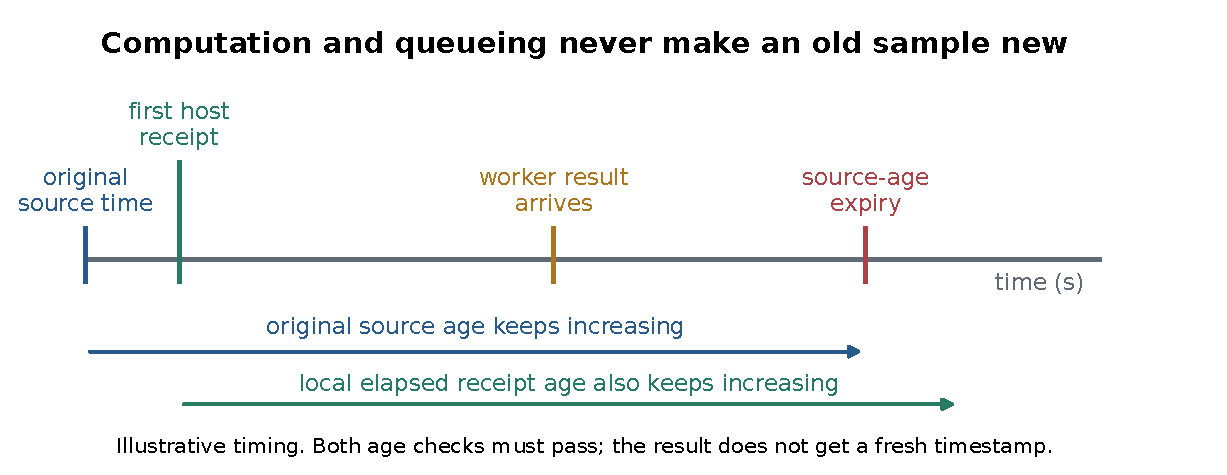
\includegraphics[width=1\linewidth,height=\textheight,keepaspectratio,alt={An asynchronous result retains the original observation age. Queueing and completion do not renew freshness.}]{v3/report_figures/timing_contract.pdf}
\caption{An asynchronous result retains the original observation age.
Queueing and completion do not renew freshness.}
\end{figure}

\subsubsection{Numerical work proposes; the main owner
decides}\label{numerical-work-proposes-the-main-owner-decides}

Coherence quadrature and fill design run in one private numerical
process. Runtime has one in-flight immutable job and no growing FIFO.
Coherence budget is 0.5 s; fill computation budget is 5 s; fitting
support is at most 4000 samples. A fill's overall design timeout starts
when DESIGN starts, so waiting for the busy/unavailable worker does not
extend that research budget.

Coherence work is keyed by search epoch, objective revision and source
stamp, with rolling's reset sequence also checked. Fill work
additionally matches candidate identity and registry generation. The
worker returns a proposal; it owns no mutable runtime registry, command
publisher or source acquisition authority. The main core accepts only a
still-relevant result and applies fill/objective changes on a
\textbf{new actual observation} while current pose and observation
geometry remain inside the candidate neighborhood.

Quadrature has finite per-segment evaluation budgets of 2048 and
current-window budget 20000. Harmonic search uses fixed finite periods
and cached designs; fill escalation has a five-round cap and 41-by-41
grids. Failing expensive research computation leaves fresh basic control
available. These design choices control callback responsiveness and
bound numerical work; they do not establish Raspberry Pi performance or
hardware stopping by themselves.

\emph{Source:
\path|ros2_ws/src/ros_esc/ros_esc/gesc_v3/core.py:194-201,329-366,447-461,548-560|;
\path|ros2_ws/src/ros_esc/ros_esc/gesc_v3/numerics/rolling.py:177-197,403-419|;
\path|ros2_ws/src/ros_esc/ros_esc/gesc_v3/numerics/coherence.py:20-27,52-65|;
\path|ros2_ws/src/ros_esc/test/test_v3_core.py:267-288,335-344,396-459,877-887|.}

\subsection{Active settings and retained helper
functionality}\label{active-settings-and-retained-helper-functionality}

\subsubsection{Read the selected owner, not a plausible
default}\label{read-the-selected-owner-not-a-plausible-default}

The current Gazebo controller JSON owns gains, velocity caps, assistance
choice and affine magnitude. Profile resolution reads that JSON and
copies its actual values into the node's
\passthrough{\lstinline!CoreConfig!}. Thus inspecting
\passthrough{\lstinline!CoreConfig()!} alone gives an incorrect
description of the selected Gazebo run.

{\def\LTcaptype{none} % do not increment counter
\begin{longtable}[]{@{}
  >{\raggedright\arraybackslash}p{(\linewidth - 4\tabcolsep) * \real{0.2727}}
  >{\raggedleft\arraybackslash}p{(\linewidth - 4\tabcolsep) * \real{0.3636}}
  >{\raggedleft\arraybackslash}p{(\linewidth - 4\tabcolsep) * \real{0.3636}}@{}}
\toprule\noalign{}
\begin{minipage}[b]{\linewidth}\raggedright
Quantity
\end{minipage} & \begin{minipage}[b]{\linewidth}\raggedleft
Generic helper/core default
\end{minipage} & \begin{minipage}[b]{\linewidth}\raggedleft
Active Gazebo choice
\end{minipage} \\
\midrule\noalign{}
\endhead
\bottomrule\noalign{}
\endlastfoot
Forward cap & 0.05 m/s & 0.10 m/s \\
Angular cap & 0.30 rad/s & 0.50 rad/s \\
Affine magnitude & 0.5 & 2.0 \\
Forward/yaw gains & 0.5 / 5.0 & 0.5 / 5.0 \\
Direct assistance & false & false \\
Assistance window/path & 15 s / 0.20 m & 15 s / 0.20 m \\
Estimator minimum sample count & 40 & 20 \\
Gaussian width floor & 0.15 m & 0.50 m \\
Gaussian amplitude cap & 3.0 & 6.25 \\
Gaussian exit multiplier & 2.5 & 2.7 \\
Affine maximum age & 30 s in standalone term & Disabled for active
escape \\
\end{longtable}
}

The selected profile also supplies 5 Hz acquisition, nominal 20 RPM arm
rate, 0.18 m sensor radius, 20 Hz command cadence, 0.5 s essential input
expiry and 4000-sample fit maximum. The 54-degree calibration is a
physical acquisition contract; an already calibrated observation or a
Gazebo joint must not receive that offset a second time. The physical V3
selected caps are separately 0.05/0.30, as recorded by the
environment/physical documents. Simulation selection does not authorize
changing hardware settings.

\emph{Source:
\path|ros2_ws/src/ros_esc/config/profiles/assets/gesc_v3/controller.json:4-17|;
\path|ros2_ws/src/ros_esc/config/profiles/algorithms.json:178-203|;
\path|ros2_ws/src/ros_esc/ros_esc/profiles.py:70-83|;
\path|ros2_ws/src/ros_esc/ros_esc/gesc_v3/node.py:65-78|;
\path|ros2_ws/src/ros_esc/ros_esc/gesc_v3/records.py:71-108|;
\path|ros2_ws/src/ros_esc/ros_esc/gesc_v3/core.py:383-387,433-439|;
\path|docs/environment_parameters.md|, active V3 table and calibration
paragraph.}

\subsubsection{Existence in a module is not active runtime
selection}\label{existence-in-a-module-is-not-active-runtime-selection}

{\def\LTcaptype{none} % do not increment counter
\begin{longtable}[]{@{}
  >{\raggedright\arraybackslash}p{(\linewidth - 4\tabcolsep) * \real{0.3333}}
  >{\raggedright\arraybackslash}p{(\linewidth - 4\tabcolsep) * \real{0.3333}}
  >{\raggedright\arraybackslash}p{(\linewidth - 4\tabcolsep) * \real{0.3333}}@{}}
\toprule\noalign{}
\begin{minipage}[b]{\linewidth}\raggedright
Mechanism
\end{minipage} & \begin{minipage}[b]{\linewidth}\raggedright
Active V3 behavior
\end{minipage} & \begin{minipage}[b]{\linewidth}\raggedright
Retained capability or caution
\end{minipage} \\
\midrule\noalign{}
\endhead
\bottomrule\noalign{}
\endlastfoot
Instantaneous GESC & Called on each accepted source observation & Helper
golden fixture alone does not include core startup priming \\
Rolling/coherence & Current one-revolution mean, three-cycle warmup,
75\% qualified blend & Sector counters are telemetry, not selected
steering density gates \\
Recurrent detector & Static, two circle supports and two harmonic
supports & Historical centroid field names do not mean the two-block
detector is active \\
Moving evidence & Three raw qualified/comparable cycles and signed
quality checks & \passthrough{\lstinline!informative!} amplitude check
is diagnostic under selected readiness policy \\
Gaussian registry & Main-thread staged immutable commit, one active fill
selected & Generic association/revision tools can do more than current
profile requests \\
Approach continuity & Newest outside anchor; enabled sufficiently
displaced interior fallback & \path|preferred_escape_direction|
opposite-approach/bounds helper is not selected \\
Escape steering & Shaped-cost GESC; optional signed normal-controller
pulse & \passthrough{\lstinline!recenter\_command!} is not called by
active core \\
Bounds/corridor geometry & Verification/design sweep checks prior
mathematical fills & Active escape receives no room bounds and no
other-fill list \\
Confidence threshold & Quality telemetry & Generic 0.60 threshold is not
an active commit gate \\
End of ordinary run & Operator interruption & A best-source event does
not hold or stop the robot \\
\end{longtable}
}

Two comments in retained code can otherwise mislead a reader.
\passthrough{\lstinline!escape.py!}'s introductory language and
numerical README still describe a heading-based inherited command law;
that refers to the retained \passthrough{\lstinline!recenter\_command!}
helper, while current direct assistance explicitly uses signed
translation through \path|Directional_Controller|.
\passthrough{\lstinline!evidence.py!} refers to separate
``supervisor/fill owners'' in its policy comment; current active
ownership is the single local core. The function bodies and their actual
call sites resolve these differences.

\emph{Source:
\path|ros2_ws/src/ros_esc/ros_esc/gesc_v3/numerics/README.md:46-60|;
\path|ros2_ws/src/ros_esc/ros_esc/gesc_v3/numerics/escape.py:1-5,536-546,593-653,744-795|;
\path|ros2_ws/src/ros_esc/ros_esc/gesc_v3/numerics/evidence.py:439-451|;
active call sites
\path|ros2_ws/src/ros_esc/ros_esc/gesc_v3/core.py:368-399,493-537|;
\path|ros2_ws/src/ros_esc/test/test_v3_core.py:812-818|.}

\subsection{Executable mental model and questions to
rehearse}\label{executable-mental-model-and-questions-to-rehearse}

\subsubsection{Pseudocode for the active
core}\label{pseudocode-for-the-active-core}

The following is explanatory pseudocode; exception/telemetry details are
abbreviated. It preserves the important separation between source
observation arrival, odometry arrival and command timer.

\begin{lstlisting}
ON FRESH ODOMETRY:
    reject invalid, old, duplicate or incompatible frame data
    count assisted path only across observed uninterrupted odometry
    append observed base pose
    if SEARCH and essential input is fresh:
        update recurrent detector at actual odometry rate
        on confirmed geometry: freeze a candidate; activity = VERIFY

ON ACCEPTED NEW SENSOR OBSERVATION:
    reject invalid age, support, frame, source or sequence data
    handle gap/reconnect without extending any original age
    if escape completion was pending: remove affine; return to SEARCH
    if a relevant fill proposal is ready and current/source poses qualify:
        stage and commit fill locally; reset objective history; begin ESCAPE
    compose objective at observed sensor position and original source time
    on startup only: prime baseline from first observed cost
    demodulate with measured body phase; update world rolling history
    add raw-cost evidence and base-position basin sample separately

ON 20 HZ STEADY-CLOCK COMMAND TICK:
    terminal state -> zero
    essential input expired -> recoverable WAITING_INPUT and zero
    poll optional worker; never let an old result renew source age
    evaluate fresh usable direction with current fresh yaw
    if direction unavailable -> WAITING_INPUT and zero
    if VERIFY: test neighborhood, measured translation and raw evidence
    if DESIGN: test finite design budget, neighborhood and translation
    submit one relevant numerical job when worker can accept it
    VERIFY/DESIGN -> moving centered tracking, with mathematical fill sweep
    ESCAPE -> measured radial progress, optional one-shot assist, shaped GESC
    SEARCH -> ordinary raw-plus-fill GESC
    reject nonfinite controller output; clip signed velocity; publish
\end{lstlisting}

\emph{Source:
\path|ros2_ws/src/ros_esc/ros_esc/gesc_v3/core.py:119-240,329-570|;
\path|ros2_ws/src/ros_esc/ros_esc/gesc_v3/node.py:94|, steady-clock
timer construction.}

\subsubsection{An explanatory walk through one
candidate}\label{an-explanatory-walk-through-one-candidate}

Initially there is no fill. The first valid brightness reading
establishes the washout baseline. A changing fresh reading supplies
instantaneous GESC motion. After three actual world-angle revolutions, a
coherent mean can stabilize steering; it was not required for startup.

Suppose observed odometry then circles a stable center. The circle
branch needs complete support and consecutive passing fits before
nominating. The candidate is not yet a declared source. The core
approaches within 8 cm and follows its 3 cm base reference while
obtaining raw cycles. A fit job is created only when three
sector-covered comparable cycles and a valid negative raw interval are
available. The base keeps moving during DESIGN; numerical preparation
does not own commands.

The worker filters support, finds a low-cost weighted center, measures
sample spread, fits a quadratic, builds a positive hill, and checks its
fitted grid for residual minima. A successful result waits for a new
actual observation. Main-thread commit verifies still-matching context,
current/source neighborhood and registry generation. Then
Gaussian-plus-affine escape uses a direction justified by observed
approach history.

The robot must show observed radial exit and hold. Completion is applied
at a subsequent real source observation; raw-plus-Gaussian searching
resumes with a new objective revision. A later distinct verified
candidate can yield a best-source event by strict raw interval
comparison. The ordinary run still continues until interrupted.

At each step, explain what is measured, what is inferred and what is
artificial: \textbf{measured} cost/pose/phase; \textbf{inferred}
direction, recurrence, weighted basin model and ranking;
\textbf{artificial} Gaussian and affine cost. This vocabulary prevents a
listener from mistaking fitted geometry for known source truth.

\emph{Source:
\path|ros2_ws/src/ros_esc/ros_esc/gesc_v3/core.py:119-240,347-460,508-538|;
\path|ros2_ws/src/ros_esc/ros_esc/gesc_v3/numerics/fill.py:81-144|.}

\subsubsection{Checks for genuine
understanding}\label{checks-for-genuine-understanding}

A reader should be able to explain why a positive Gaussian assists
minimization; why the affine dot product has a negative sign; why a
first absolute voltage reading is not a measured gradient; why averaging
body vectors during yaw changes is wrong; why current rolling mean and
three-cycle raw evidence serve different purposes; why poor fit
confidence and loss of fresh control are different conditions; and why a
best-source event does not prove global convergence.

For debugging, identify which boundary failed before changing a gain. No
motion can come from a zero demodulated direction, stale input, expired
worker context, tracking geometry, controller component projection or
terminal integrity state. No fill can come from incomplete raw phase
sectors, incomparable base trajectories, raw sign/quality failure,
insufficient filtered support, a residual fitted grid minimum, stale
generation or departure during DESIGN. These mechanisms have explicit
event reasons and focused tests. A plot of raw cost alone cannot tell
them apart.

The golden numerical fixtures compare selected helper calculations with
retained pre-refactor values. Focused tests add startup priming,
candidate cancellation, stale result rejection, objective transition,
selected raw-off escape, assist consumption and continuous fresh input
recovery. They establish specified software behavior under constructed
inputs. Whether an actual Gazebo or physical trajectory exercises those
paths is a separate evidence question covered by the run chapters of
this report.

\emph{Source:
\path|ros2_ws/src/ros_esc/test/test_v3_numerics.py:1-5,115-279|;
\path|ros2_ws/src/ros_esc/test/test_v3_core.py:1-5,87-288,396-459,478-527,564-771,794-1005|;
\path|ros2_ws/src/ros_esc/test/test_v3_direction_handoff.py:32-125|.}

\section{Evidence, development history, simulation results and physical
continuation}\label{evidence-development-history-simulation-results-and-physical-continuation}

\subsection{Report identity and how to interpret its
claims}\label{report-identity-and-how-to-interpret-its-claims}

This report describes the active GESC + Gaussian \textbf{V3 algorithm}
in the clean \passthrough{\lstinline!refactor/esc-v3!} checkout, with
runtime commit \path|34927997ab33c3fd483e6d461e9470e961ba7bbc| and
documentation commit/current HEAD
\path|2be0bad33a314f7b383d65f4bab876d401b7c888|. The published closeout
on 2026-10-01 local time records equality of local, upstream and remote
branch hashes, zero ahead/behind counts, and a clean tree. Those
remote/publication observations belong to the retained closeout; the
report also inspected the present local Git tree, which was clean before
authoring. This report does not make a fresh remote-Pi-state claim.
{[}ES01, ES02{]}

The user's decision on 2026-10-05 is that the \textbf{simulation/Gazebo
algorithm is satisfactory}. That is the current project decision: this
report teaches and documents the working simulation result instead of
treating an unfinished statistical qualification programme as an
instruction to resume it. It preserves the narrower scientific
descriptions of the actual records. Selected Gazebo trials demonstrate
Gaussian filling, local escape without direct heading assistance,
resumed SEARCH and stronger-source vicinity. They do not establish
universal convergence, a calibrated Arduino/servo observation model,
statistical repeatability, or physical Gaussian escape. The selected
affine-2.0 Gazebo run predates the subsequent worker-initialization,
accepted-direction handoff and initial-filter-priming corrections; those
corrections have software and Pi recorded-input replay evidence, plus
later SEARCH-only physical observation, but no subsequent recorded
Gazebo trial is identified by the current authority documents. {[}ES03,
ES04, ES13, ES22, ES23{]}

Four different questions must be kept separate when explaining a result:

{\def\LTcaptype{none} % do not increment counter
\begin{longtable}[]{@{}
  >{\raggedright\arraybackslash}p{(\linewidth - 4\tabcolsep) * \real{0.3333}}
  >{\raggedright\arraybackslash}p{(\linewidth - 4\tabcolsep) * \real{0.3333}}
  >{\raggedright\arraybackslash}p{(\linewidth - 4\tabcolsep) * \real{0.3333}}@{}}
\toprule\noalign{}
\begin{minipage}[b]{\linewidth}\raggedright
Question
\end{minipage} & \begin{minipage}[b]{\linewidth}\raggedright
What counts as evidence
\end{minipage} & \begin{minipage}[b]{\linewidth}\raggedright
An example of an invalid shortcut
\end{minipage} \\
\midrule\noalign{}
\endhead
\bottomrule\noalign{}
\endlastfoot
Did the source/software behave as specified? & Tests, installed
import/resource checks, source hashes, actual isolated ROS checks &
Calling 311 passing software checks proof of physical convergence \\
Did the simulated research behavior occur? & Closed-bag commands, pose,
fill and event chronology under pinned configuration & Calling a fill
proposal an activated fill, or calling source vicinity autonomous source
identification \\
Is the recording usable/complete? & Required topics and honest
availability, closure, source identity, original validator result where
applicable & Relabeling a V2 completeness-FAIL run because its
trajectory looks successful \\
Did the physical robot do it? & Operator observation plus appropriate
physical data, timing and geometry & Calling raised-wheel odometry
translation, or GPIO neutral a measured stationary interval \\
\end{longtable}
}

The historical phrase ``Phase 08 v3'', or ``v3B/v3D'' in the V1 report,
names versions of that \textbf{older experiment suite}. It is not the
active V3 refactor introduced in September 2026. Frozen V1 and V2
reports describe their original architectures and evidence. Their
supervisor/recorder/ACK mechanisms must not be read as current V3
runtime components. {[}ES05, ES06{]}

\subsection{Why V3 followed V1 and V2}\label{why-v3-followed-v1-and-v2}

V1 established a typed Gaussian-assistance architecture and selected
two-basin feasibility. Its strongest recorded simulation results were
11/11 formal passes in the fixed primary layout, 6/6 in a fixed
secondary layout and 14/14 formal predicates in the selected visible
case. A varied case remained 13/14 because measured exit alignment was
below its declared threshold, with three seeds withheld. The retained
earlier physical success exercised fill, escape and reacquisition but
did not establish second-source confirmation or GOAL\_HOLD and remained
61/62 complete. V1 is therefore a selected-case foundation, preserved at
\passthrough{\lstinline!1af67c6!}, not broad validation. {[}ES05,
ES06{]}

V2 retained measured-angle rolling GESC and moving raw-cost verification
and investigated alternative detectors. The user accepted Test D
simulation at frozen \passthrough{\lstinline!d1779b6!}; GOAL\_HOLD
stayed implemented but was not required for arrival acceptance. A later
5 Hz/20 RPM selected experiment, preserved separately at
\passthrough{\lstinline!e726774!}, demonstrated one fill, assisted
escape and global-region arrival at 185.327 simulated seconds. Its
unchanged original strict completeness was \textbf{FAIL}, and its
successful fill used established invalid-quadratic handling because a
condition number near 1.560e8 exceeded the 1e8 limit. Arrival and
numerical quality were explicitly separate conclusions. Physical V2
acquisition remained 0/3 qualified and was paused. These facts motivated
V3; they are not retroactively successful V3 tests. {[}ES07, ES08{]}

The initial V3 fault inventory found that a generic terminal FAILSAFE
label combined very different events: deliberate stopping, temporarily
unavailable input, synchronization errors, research fitting problems,
recorder failures and some strategy timeouts. Historical
synchronization/filter recovery could still lead to a terminal
integrated supervisor latch. V3 addressed both computational and
ownership complexity: one authoritative observation, one
controller-owned algorithm core, one optional bounded numerical worker,
local objective/registry transactions, optional independent recording
and simpler recoverable data behavior. The inventory was a
planning/source audit, not evidence that every listed historical fault
occurred in one run. {[}ES09, ES10{]}

The retained physical evidence also explained why merely increasing
sampling rate or adding orchestration was inadequate. Healthy restored
V1 measured about 4.978 Hz and 17.176 RPM despite nominal 20 RPM. At 5
Hz/20 RPM, a nominal revolution contains 15 samples; at 17.2 RPM it
contains about 17.4. Sparse angular evidence has to be evaluated
honestly. In historical live V2 records, support geometry, callback
delays, recording/CPU load and source/install selection were distinct
problems. The fixed approximately 5 Hz UNO application was a
firmware/application choice, not proof that the ADC was intrinsically
incapable of faster conversion. V3 preserves unknown acquisition timing
instead of inventing device timestamps. {[}ES09, ES10{]}

\subsection{Refactor and preservation
checkpoint}\label{refactor-and-preservation-checkpoint}

The accepted refactor plan of 2026-09-28 superseded the earlier planning
topology. It explicitly retained the original ESC methods, interactive
Gazebo Matplotlib plots and external physical adapters. It removed the
distributed Gaussian supervisor/composer/detector/fill ROS choreography
from the active V3 path while preserving the underlying selected
numerical ideas. Ordinary simulation aliases resolve installed profiles
and launch without rebuilding or editing JSON. Physical commissioning
later received a distinct authorized build/source/launch rule.
{[}ES11{]}

The software refactor's preservation evidence includes 2,930
pre-refactor entries archived with verified contents, modes and
symlinks; 523 obsolete active files retained externally with destination
hashes; 1,437 generated tracked entries removed; unchanged frozen
references; a fresh three-package symlink workspace build; and an
installed suite of \textbf{196 passed, no skips, 9.04 seconds}. Exactly
eight simulation interfaces, nineteen aliases and eleven intended
console entries were inventoried at that checkpoint. Original-profile
numerical comparisons and isolated real ROS
subprocess/expiry/recovery/SIGINT checks were part of the software
evidence. These counts belong to that checkpoint and are not the current
test total or physical interface inventory. {[}ES12{]}

The audit corrected several implementation issues before closure:
selected gain and centered phase, repulse-to-assist ordering, known-fill
suppression, both current-pose and incoming-observation neighborhood
checks at commit, detector boundary timestamps and full-rate odometry
detector input. Compatibility repairs included intended scalar
Lie-bracket input, finite recoverable legacy filter reset and proper
unknown rotation-direction initialization. Golden traces supported
selected numerical equivalence; no universal trajectory equivalence was
claimed. Intermediate failing checks were retained. {[}ES12{]}

\subsection{Gazebo development ledger: failed pilots remain
informative}\label{gazebo-development-ledger-failed-pilots-remain-informative}

The first pilot used approximately 5 Hz modeled cost, nominal 20 RPM and
initially physical-target caps 0.05 m/s and 0.30 rad/s. ADC matching was
disabled and there was no noise. This was an idealized integration
baseline, not a calibrated physical simulator. Runs were isolated on
localhost with finite outer wall deadlines, one live graph at a time;
GUI/live Matplotlib was retained for interactive cases. No physical
operation accompanied the Gazebo work. {[}ES13{]}

{\def\LTcaptype{none} % do not increment counter
\begin{longtable}[]{@{}
  >{\raggedright\arraybackslash}p{(\linewidth - 4\tabcolsep) * \real{0.3333}}
  >{\raggedright\arraybackslash}p{(\linewidth - 4\tabcolsep) * \real{0.3333}}
  >{\raggedright\arraybackslash}p{(\linewidth - 4\tabcolsep) * \real{0.3333}}@{}}
\toprule\noalign{}
\begin{minipage}[b]{\linewidth}\raggedright
Retained case
\end{minipage} & \begin{minipage}[b]{\linewidth}\raggedright
Configuration and direct outcome
\end{minipage} & \begin{minipage}[b]{\linewidth}\raggedright
Interpretation
\end{minipage} \\
\midrule\noalign{}
\endhead
\bottomrule\noalign{}
\endlastfoot
Run01, \path|run01_visible_baseline| & Shell nounset error in ROS setup
before graph startup & Prelaunch infrastructure failure; no algorithm
observation \\
Run02, \path|run02_visible_baseline| & 3,228 commands, all zero; only 2
valid observations and 9,972 invalid notices, mostly future pose/phase;
no ACTIVE & Integrated clock-delivery failure. Gazebo /clock was 10 Hz
while odometry was about 30 Hz. The 0.0522 m drift was not commanded
motion. Clock was absent from the bag due to precreated recorder QoS,
and launch-wrapper children required identity-scoped cleanup \\
Run03, \path|run03_visible_clock_correction| & 1,744 valid observations
at 4.902 Hz, 19.996 RPM, RTF 0.9953, 8.706 m path; no
candidate/fill/escape; local closest 4.9 mm, global closest 3.315 m &
Motion worked, Gaussian/global outcome failed within the fixed 360 s
case. Detector circle models achieved at most 2 consecutive passes of 3.
Further repeated-SIGINT/Gazebo-child shutdown findings were retained \\
Run04, \path|run04_cost_pause_recovery| & Exactly one 2.0015 s
suspension of the verified cost process; first WAITING/zero 0.361 s
after marker; fresh observation 1.61 ms and nonzero command 9.34 ms
after resume; 1.650 s zero interval; clean closure & Selected simulated
software/data-outage stop and automatic recovery. Marker-to-bag-receipt
latencies, not callback/actuator latency; not Arduino timing
qualification \\
Run05, \path|run05_measured_mean_arm_speed| & Custom constant 17.2 RPM
case, measured 17.194 RPM; candidate/VERIFY at 144.3 s, cancelled at
152.3 s by then-active eight-second approach timeout; 0.285 m measured
VERIFY path, all 163 mapped commands nonzero & Moving verification
approach occurred; no full verification/design/fill/escape/global
success. Radius declined from about 186 to 109 mm and never reached 80
mm. Fixed six-minute behavioral failure remains \\
\end{longtable}
}

Run04's zero interval contained 1.325 mm odometry travel including
deceleration, and only 0.369 mm in its final second; the next second
after resume moved 39.51 mm. It supports a selected simulated
interruption/restart. It does not satisfy uninterrupted
continuous-motion research behavior during an outage: the protective
stop is deliberately recorded as an interruption. Run05 demonstrated
translation rather than spin-only acquisition: all fifteen half-second
offline movement screens exceeded 1 mm. Those offline anchors
approximate runtime callbacks, rather than replaying their exact subset.
{[}ES13{]}

The bounded integration fixes preserved original freshness.
Simulation-leading source records wait for actual /clock delivery within
125 ms and finite 32-record per-stream storage, carrying their original
stamps and first receipt. Physical future rejection and the 0.5 s core
limit were unchanged. Recorder discovery preceded QoS selection. Direct
installed CLI executables, explicit gzserver/gzclient ownership,
deferred repeated-signal cleanup and current-monotonic evaluation of
deferred data repaired distinct integration defects. They were verified
before later versioned cases rather than rewriting failed Run02/03
outcomes. The installed suite grew through 213, 215, 222 and ultimately
228 passing checks at successive checkpoints; these overlap and must not
be summed as unique tests. {[}ES13{]}

The user then selected simulation caps 0.10/0.50 to match archived
full-rotation light GESC limits, retaining V3 gains 0.5/5 rather than
the baseline's linear gain 1.0. Arbitrary approach, total-verification
and coverage elapsed cancellations were removed, preserving the 8 cm
entry radius, neighborhood, motion, freshness and finite worker checks.
Visible light markers were restored from the selected cost JSON, with no
second coordinate source and no source truth supplied to control. Run06
began under those changes. {[}ES14{]}

\subsection{Run06: first V3 fill, assisted escape and stronger-source
vicinity}\label{run06-first-v3-fill-assisted-escape-and-stronger-source-vicinity}

Run06, retained under
\path|gazebo_speed_lights_20260928T231502Z/run06_baseline_caps_no_verification_deadline|,
was stopped after approximately one minute near the stronger source,
before its 600 s outer bound. It was an observation stop, not
predeclared statistical convergence. Candidate/VERIFY began at 78.7
simulated seconds; DESIGN at 89.8; fill 1 committed and ESCAPE began at
90.0; stalled progress invoked the then-selected direct assistance at
93.9; measured \passthrough{\lstinline!escape\_complete!} occurred at
108.8; a real observation applied SEARCH at 109.0. Final
SIGINT/STOPPED/zero occurred at 349.4. {[}ES14{]}

The fill's center was about 9.37 cm from the configured local source,
amplitude 0.1, principal widths about 0.5062 m and exit radius about
1.3668 m. VERIFY measured 0.366 m path over 11.1 s, with all 21
half-second screens above 1 mm. DESIGN translated 3.25 mm over its short
0.17 s recorded segment; its 0.2 s state duration cannot establish a
full half-second movement screen. ESCAPE completed in 18.8 s, before the
then-active 35 s cutoff, with assistance. Closest stronger-source
distance was about 0.865 mm, final distance 146.4 mm. No best\_source
event occurred. {[}ES14{]}

The source review after Run06 removed the remaining 35 s ESCAPE
return-to-SEARCH transition and coupled affine age cutoff. The
mathematical affine decay and generic helper defaults remained. Later
regressions demonstrated long-lived escape and later measured spatial
exit, with stale inputs and integrity faults still inhibiting motion.
Run06 finished before either removed cutoff, so it remains evidence
under its original source, not a test of the later policy. The final
installed suite for this development checkpoint was 240 passed, no
skips. {[}ES14{]}

\subsection{Unassisted escape, affine comparison and the selected 2.0
result}\label{unassisted-escape-affine-comparison-and-the-selected-2.0-result}

The direct-assistance-disabled pilot retained nominal 5 Hz/20 RPM, gains
0.5/5, caps 0.10/0.50, field/start and affine 0.5. Its bag
\path|20260929T005716.079166Z-47151| recorded VERIFY at 78.5 s, DESIGN
94.1, fill/ESCAPE 94.3, escape\_complete 116.1 and SEARCH 116.3, then
observation stop at 236.9. All 444 clock-mapped escape commands, or 442
under the event-receipt boundary method, translated; zero
direct-assistance events were recorded. Measured escape path was 2.001 m
and completion took 21.8 s. All 43 half-second measured escape screens
exceeded 1 mm, minimum 6.45 mm. Final global distance was 22.38 mm. A
short progress-stall flag could occur without requiring direct
assistance: continued Gaussian-plus-affine GESC still completed escape.
{[}ES15{]}

The user requested a single tenfold affine comparison, 5.0 versus 0.5,
with assistance still off. Bag \path|20260929T011459.310299Z-50159|
recorded candidate 276.4 s, DESIGN 279.3, fill 279.6, completion/SEARCH
300.0 and observation stop 413.1. Escape took 20.4 s and 1.880 m
measured path. Linear/angular saturation increased to 96.11\%/95.62\%,
with 27 signed linear-command reversals, versus 84.16\%/64.71\% and 25
at 0.5. Final global distance was 84.55 mm. The longer initial circling
occurred before affine activation, so it cannot be explained as the
escape coefficient already steering SEARCH. Different candidate
histories/fill centers prevent a clean isolated causal estimate of the
coefficient's benefit. {[}ES16{]}

The user then selected affine \textbf{2.0}, retaining assistance off and
all other settings, and authorized exactly one final evening run. The
preserved source checkpoint was \passthrough{\lstinline!a702cd2!}, bag
\path|20260929T013734.407314Z-52815|, at evidence root
\path|affine_2_20260929T013558Z|. Its manifest pins 215 runtime files
and six external configuration files; cleanup/source-pin checks report
no changed pins, clean process exits and finalized recording. {[}ES17,
ES18{]}

{\def\LTcaptype{none} % do not increment counter
\begin{longtable}[]{@{}
  >{\raggedleft\arraybackslash}p{(\linewidth - 2\tabcolsep) * \real{0.5714}}
  >{\raggedright\arraybackslash}p{(\linewidth - 2\tabcolsep) * \real{0.4286}}@{}}
\toprule\noalign{}
\begin{minipage}[b]{\linewidth}\raggedleft
Simulated time
\end{minipage} & \begin{minipage}[b]{\linewidth}\raggedright
Selected affine-2.0 chronology
\end{minipage} \\
\midrule\noalign{}
\endhead
\bottomrule\noalign{}
\endlastfoot
144.7 s & Recurrent candidate confirmed; moving VERIFY \\
149.9 s & DESIGN begins with 46 evidence samples \\
150.2 s & One Gaussian fill committed; ESCAPE begins \\
171.647 s & Recorded odometry first crosses exit radius \\
172.667 s & Offline spatial replay reaches stable exit \\
172.8 s & Runtime escape\_complete \\
173.0 s & Next real observation applies SEARCH \\
204.389 s & First within 0.5 m of stronger source, staying inside
afterward \\
293.1-306.2 s & Moving candidate verification/ranking near stronger
source, then SEARCH \\
297.991 s & First within 0.10 m, staying inside afterward \\
319.3 s & Agent observation stop; STOPPED/final zero \\
\end{longtable}
}

The committed fill had center
\path|(0.628620133983457, 1.4156102850203167)| m, amplitude 0.1, equal
principal widths 0.5062114183 m, support radius 1.5186342548 m and exit
radius 1.3667708294 m. Forty samples remained in the fitted record;
confidence was about 0.7411, fit residual about 0.000200709 and reported
condition number about 4.433e6. These are actual published numerical
diagnostics, not a universal fitting-quality guarantee. {[}ES18, ES19{]}

ESCAPE took \textbf{22.6 s to the completion event} and 22.8 s until
SEARCH applied. Measured path was 2.096957 m and net displacement
1.439257 m. All 458 event-bounded escape commands had nonzero
translation, with no turn-only samples or assistance events; all 44
half-second recorded-pose screens exceeded 1 mm, minimum 4.487 mm. There
were 32 signed command reversals; they are direction changes in GESC
commands, not measured stops. VERIFY and the short DESIGN segment also
translated. Offline recorded geometry corroborated the runtime
stable-exit transition; it samples all recorded odometry rather than the
exact runtime callback subset. {[}ES19{]}

The final stronger-source distance was \textbf{0.023327 m}, with the
final \textbf{21.352 s inside 0.10 m}. A live probe had shown an orbit
roughly 0.21-0.33 m away, but the closed record showed a later inward
movement; the final report uses the closed data. The user's 20-30 cm
acceptable-vicinity preference was met before that inward movement. No
best\_source event was recorded, so this is observed stronger-source
approach/vicinity, not verified autonomous ranking or automatic goal
hold. There was final zero and clean process closure; only one odometry
receipt followed zero, about 9.67 ms later, which is insufficient to
establish a measured stationary stopping interval. {[}ES17-ES19{]}

{\def\LTcaptype{none} % do not increment counter
\begin{longtable}[]{@{}lrrr@{}}
\toprule\noalign{}
Metric & Affine 0.5 & Selected 2.0 & Affine 5.0 \\
\midrule\noalign{}
\endhead
\bottomrule\noalign{}
\endlastfoot
Escape completion elapsed & 21.8 s & 22.6 s & 20.4 s \\
Escape measured path & 2.001 m & 2.097 m & 1.880 m \\
Linear commands at cap & 84.16\% & 92.79\% & 96.11\% \\
Angular commands at cap & 64.71\% & 91.27\% & 95.62\% \\
Signed linear-command reversals & 25 & 32 & 27 \\
First candidate time & 78.5 s & 144.7 s & 276.4 s \\
\end{longtable}
}

This is a three-case development comparison, each with one execution and
different pre-escape histories. It does not show monotonic performance
improvement or prove one magnitude generally optimal. Affine activation
follows the candidate/fill, so candidate-time variability remains a
separate SEARCH/detector issue. The user selected 2.0 and considers the
simulation algorithm satisfactory; the recorded evidence supplies the
concrete demonstration behind that decision. {[}ES17-ES19{]}

\begin{figure}
\centering
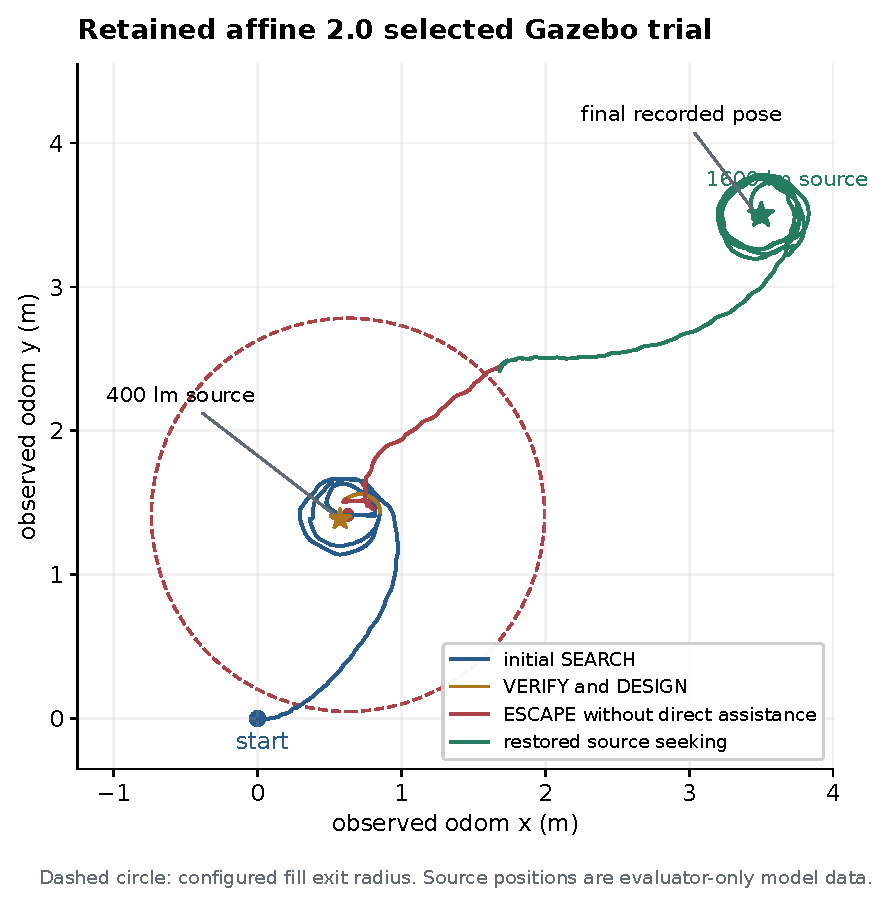
\includegraphics[width=0.9\linewidth,height=\textheight,keepaspectratio,alt={Retained selected affine-2.0 Gazebo odometry, source-model evaluator positions, and fill exit radius. The trial predates later shared steering corrections.}]{v3/report_figures/gazebo_route.pdf}
\caption{Retained selected affine-2.0 Gazebo odometry, source-model
evaluator positions, and fill exit radius. The trial predates later
shared steering corrections.}
\end{figure}

\subsection{What simulation has and has not
established}\label{what-simulation-has-and-has-not-established}

The successful cases establish selected two-source/one-fill
functionality, cost-shaped unassisted escape, moving
verification/design/escape, recovery from one selected simulated input
interruption, recorded final-zero emission and eventual clean isolated
launch closure. Selected rates were around 4.902 Hz, with
nominal/observed simulated arm near 20 RPM and near-real-time factor
about 0.994-0.995. They do not identify a physical acquisition-delay
distribution, reproduce actual nonuniform servo loading, calibrate
photoresistor optics, show broad seeds/layouts/noise/backlog/resource
robustness, qualify Pi full-graph headroom or quantify actuator
stopping. The inherited optional ADC matcher was explicitly disabled and
not a faithful validated UNO model. {[}ES12-ES19{]}

A sampled host CPU record from failed Run03 estimated controller+worker
about 0.153 core, adapters 0.402, recorder 0.0566 and liveplot 1.009
during the sampled coverage. It excludes startup/exit tails and is not
Pi instruction-level capacity evidence. Removing the large plot from
physical runs is architecturally useful, but those numbers must not be
presented as a physical CPU qualification. {[}ES13{]}

\subsection{Physical architecture and installed
settings}\label{physical-architecture-and-installed-settings}

Physical V3 was separately authorized on 2026-09-29. It uses the
existing Pi \passthrough{\lstinline!/home/pi/ros2\_ws!} with ordinary
copied installations, not a sibling workspace. Physical
acquisition/rotation/bringup is in external
\path|turtlebot3_vehicle_nodes|; shared algorithm code remains
\passthrough{\lstinline!ros\_esc!}, and OpenCR supplies control
\passthrough{\lstinline!/odom!}. Vicon is independent optional
evaluation. The report reads retained/offline source and artifacts; it
does not contact, mount or operate the Pi. {[}ES20, ES21{]}

The explicit operator command is:

\begin{lstlisting}[language=bash]
bash ~/ros2_ws/src/turtlebot3_vehicle_nodes/bash_scripts/light_esc_experiments/voltage_cost_values/gesc_gaussian_v3_voltage.bash
\end{lstlisting}

That physical wrapper sources underlays, performs a bounded ordinary
copied build, sources its install, then launches.
\passthrough{\lstinline!--check-only!} performs
build/source/configuration inspection without opening devices or
launching hardware. \passthrough{\lstinline!--assist!},
\passthrough{\lstinline!--no-record!},
\passthrough{\lstinline!--no-vicon!},
\passthrough{\lstinline!--output!}, serial-device and OpenCR-device
overrides are available. The operator-run itself has no elapsed
termination deadline; Ctrl+C owns termination. The generic Gaussian
command has not been silently promoted to V3, and the old V1-only build
wrapper is preserved in backup. {[}ES21, ES24{]}

{\def\LTcaptype{none} % do not increment counter
\begin{longtable}[]{@{}
  >{\raggedright\arraybackslash}p{(\linewidth - 4\tabcolsep) * \real{0.3333}}
  >{\raggedright\arraybackslash}p{(\linewidth - 4\tabcolsep) * \real{0.3333}}
  >{\raggedright\arraybackslash}p{(\linewidth - 4\tabcolsep) * \real{0.3333}}@{}}
\toprule\noalign{}
\begin{minipage}[b]{\linewidth}\raggedright
Selected setting
\end{minipage} & \begin{minipage}[b]{\linewidth}\raggedright
Gazebo
\end{minipage} & \begin{minipage}[b]{\linewidth}\raggedright
Last verified physical/offline source
\end{minipage} \\
\midrule\noalign{}
\endhead
\bottomrule\noalign{}
\endlastfoot
Forward/angular gain & 0.5 / 5.0 & 0.5 / 5.0 \\
Linear/angular cap & 0.10 m/s / 0.50 rad/s & \textbf{0.05 m/s / 0.30
rad/s}, reduced after first floor review \\
Affine magnitude & 2.0 & 2.0 \\
Direct escape assistance & Off & Off; optional one 20 cm measured-path
pulse after \textless5 cm outward progress in 15 s \\
Acquisition & Modeled nominal 5 Hz; observed about 4.902 Hz in selected
run & Original fixed approximately 5 Hz UNO application, 9600 baud \\
Arm & Nominal 20 RPM; simulated observation about 19.98 RPM & Nominal 20
RPM; latest actual observed about 17.07 RPM \\
Calibration & Gazebo joint angle, no physical offset added & 54 degrees
applied once in acquisition \\
Clock and pose & ROS simulated time, observed /odom & System time,
OpenCR /odom \\
Vicon & Not required & Optional evaluation only \\
Plot/recording & Interactive Matplotlib; optional standard bag & No
physical plot; optional standard bag and Vicon \\
\end{longtable}
}

There is \textbf{no SSH-loss/session/network monitor}, no
recorder-readiness gate, no research supervisor and no timer to end
normal approach, verification, escape or the overall operator run. This
does not remove essential input age or local process/actuator stopping
checks. {[}ES20, ES21{]}

The physical observation adapter reads serial without writing firmware
or issuing sampling-rate commands. It assigns complete-line \textbf{host
receipt time}, never an ADC acquisition time or invented device
sequence. Cost is \passthrough{\lstinline!-voltage!}. Genuine feedback
edges on GPIO23 supply calibrated phase; cached angle does not renew
edge freshness. The shared ObservationBuilder assembles observed
pose/phase/cost with 0.18 m sensor radius, 0.5 s expiry and 0.05 s
support tolerance. Nonblocking serial work has finite
buffer/partial-line/polling bounds and recoverable reopen.
Pending-support notices can precede a later valid assembled observation:
their count is not automatically a lost-sensor-sample count.
{[}ES25-ES27{]}

The small physical process owner uses a local authenticated Unix socket
to observe completed controller/acquisition loops, Linux parent-death
binding to actual child executables, a single GPIO18 command owner and a
pigpiod-resident servo expiry script. The current physical lease is
\textbf{1.0 s}, distinct from archived V45 values. Expiry writes 1500
microseconds neutral and HALTs; it does not rearm after tick wrap.
Optional recorder/Vicon failures report and continue. Ordinary missing
data requests recoverable zero/arm neutral while completed
acquisition/control execution can remain alive; a stopped critical
execution loop is a different fault. Emergency shutdown stops the driver
first; normal Ctrl+C allows final-zero publication before driver
shutdown. These are software mechanisms with selected test evidence, not
proof of pigpiod/OS/electrical robustness. {[}ES28{]}

\subsection{Deployment, raised-wheel stopping and
preservation}\label{deployment-raised-wheel-stopping-and-preservation}

Before V3 replacement, all 347 V46 source files matched the live Pi.
Complete prior source/build/install was archived and independently
hash-verified on host, with original numerical dependency separately
preserved. The V1 workspace archive SHA256 is
\path|9b2297fdaeaef9958f7f6fa99cc15098ebc6979e8fa8f0a771ed79dee3985691|,
under \path|~/mbuck_backups/gesc_v3_deployment_20260929T210229Z|, with
whole-workspace restoration guidance. Firmware was left unchanged; its
identity is inherited from V46, not a new flash readback. {[}ES24,
ES29{]}

Deployment covered 393 physical source files and a fresh ordinary
three-package build. Pi-native validation recorded 222 retained legacy
tests, 170 V3 tests, then 5 terminal-fault and 17 real ROS/control/bag
tests after review. Final shared suite at that stage recorded 297
passed. All 26 legacy Bash methods remained byte-identical, original
numerical/configuration probes matched pre-deployment and 117 installed
Python runtime files/12 physical interfaces resolved correctly. These
are separate overlapping suites, not a sum of unique physical tests. An
ownership-stop gap was found and corrected: physical terminal FAULTED no
longer keeps renewing process authorization. WAITING\_INPUT remains
recoverable. {[}ES29{]}

Raised-wheel check \passthrough{\lstinline!normal\_ctrlc\_01!} failed
before hardware startup because the executable path was wrong; it
remains a failed startup. Corrected
\passthrough{\lstinline!normal\_ctrlc\_02!} measured 46 valid
observations at 4.9724 Hz and actual arm about 17.95 RPM, 9.136 s
consecutive nonzero commands, then final-zero/STOPPED and closed bag.
The operator confirmed wheels and arm stopped promptly. Raised-wheel
odometry is not translation and precise stopping latency was not
instrumented. {[}ES30{]}

{\def\LTcaptype{none} % do not increment counter
\begin{longtable}[]{@{}
  >{\raggedright\arraybackslash}p{(\linewidth - 6\tabcolsep) * \real{0.2308}}
  >{\raggedright\arraybackslash}p{(\linewidth - 6\tabcolsep) * \real{0.2308}}
  >{\raggedleft\arraybackslash}p{(\linewidth - 6\tabcolsep) * \real{0.3077}}
  >{\raggedright\arraybackslash}p{(\linewidth - 6\tabcolsep) * \real{0.2308}}@{}}
\toprule\noalign{}
\begin{minipage}[b]{\linewidth}\raggedright
Operator-observed check
\end{minipage} & \begin{minipage}[b]{\linewidth}\raggedright
Injected fault
\end{minipage} & \begin{minipage}[b]{\linewidth}\raggedleft
Observed driver process exit
\end{minipage} & \begin{minipage}[b]{\linewidth}\raggedright
Wheels and arm stopped
\end{minipage} \\
\midrule\noalign{}
\endhead
\bottomrule\noalign{}
\endlastfoot
Normal Ctrl+C & Harness SIGINT after bounded check & Normal closure &
Yes \\
Controller crash & Exact controller SIGKILL & About 0.05 s & Yes \\
Controller freeze & Exact controller SIGSTOP & About 1.03 s & Yes \\
Acquisition freeze & Exact acquisition SIGSTOP & About 1.01 s & Yes \\
Guard crash & Exact local guard SIGKILL & About 0.05 s & Yes \\
Guard freeze & Exact local guard SIGSTOP & About 1.01 s & Yes \\
\end{longtable}
}

The exit times measure observer detection/process termination,
\textbf{not wheel or arm stopping latency}. Acquisition freeze first
emitted zero at about 0.45 s, then local protection stopped the driver.
Every selected process-fault case had separate operator confirmation and
neutral/process checks before harness cleanup. Kernel, pigpiod,
electrical faults, collision protection and measured physical stop
latency remain unqualified. Finite commissioning harness bounds were not
added to ordinary V3 runtime. {[}ES30{]}

Independent Vicon was restored later without changing its legacy wire
protocol or control pose. A stationary Vicon-only check observed 123
finite poses around 9.499 Hz, with 124 in the closed bag, and no
base/arm/controller launch. The client converts wire millimeters to
meters and uses host receipt time. Its retained one-greeting/one-client
server behavior requires restarting the UDP server between runs; server
absence and process failure cannot gate V3 control. Initial floor bags
without Vicon cannot gain retrospective tracking. {[}ES31{]}

\subsection{Floor-run diagnosis and
corrections}\label{floor-run-diagnosis-and-corrections}

The first reviewed mobile floor run,
\path|20260929T203345_844703Z-3962|, had 47.75 s nonzero commands and
SEARCH only, no Gaussian fill or escape. Vicon recorded about 4.12 m
path and 3.22 m net displacement; 238 valid observations were sequential
at 4.979 Hz. Initial physical caps were still 0.10/0.50, with high
command saturation. The operator stopped for clearance in a cramped room
and reported passing the local light; unrecorded lamp coordinates
prevent quantifying that pass. The user then explicitly authorized
physical caps 0.05/0.30, preserving gains and all other settings. Gazebo
remains 0.10/0.50. {[}ES32{]}

Seven evening bags all remained SEARCH with no fills, no recorded
expiry/fault event, no internal zero-command interval and
operator\_stop/final zero. Lower-cap runs lasted 58.60/101.42/92.95 s,
with broad partial arcs and descriptive fits around 1.7-2.3 m. Their
valid observations remained consecutive. Offline recurrent-detector
replay found no candidates, with complete circle windows violating at
least the 0.5 m radius criterion. The evidence exposed a concrete Pi
numerical-worker problem rather than justifying forced filling or
arbitrary gain/calibration changes. {[}ES33{]}

\textbf{Correction 1: numerical worker initialization.} Three cold Pi
coherence jobs repeatedly exceeded their production 0.5 s allowance
because lazy SciPy import occurred after readiness/job timing began. A
diagnostic-only longer budget let the cold job complete around 0.655 s;
warm compute was about 6-8 ms. The corrected worker binds parent-death
cleanup and imports dependencies before ready. Control stays nonblocking
and can use fresh instantaneous input during worker initialization;
coherence 0.5 s/fill 5 s budgets and original age limits were not
extended. Host focused 133 and Pi installed 101 checks passed.
Fixed-input actual-Pi replay changed zero completed jobs/12 deadline
errors/zero blended ticks into 46 jobs/no errors/136 blended ticks in
400 command ticks. This demonstrated restored averaging participation,
not changed physical trajectory. {[}ES22{]}

An incremental build initially reported success while retaining old
installed worker after a backward Pi clock change left generated-cache
mtimes in the future. The regression caught this as 1 failed/100 passed.
Previous generated trees were preserved; a fresh ordinary package build
and imported-byte/hash checks repaired source/install parity. Build exit
alone was therefore insufficient evidence. The user changed the clock;
the agent did not. Pi UTC-labelled run directory times need their
recorded provenance and are not automatically synchronized host UTC.
{[}ES22{]}

\textbf{Correction 2: accepted-direction handoff and initial filter
priming.} Two post-worker-fix one-light runs,
\path|20260930T203848_419838Z-1257| and
\path|20260930T204014_854018Z-1510|, showed averaging but a new
discontinuity: an incoming observation made a pending unqualified
coherence snapshot, briefly switching to instantaneous control before
the worker result. Distinguishable early commands favored instantaneous
steering, later commands blended steering. The initial zero washout also
made the first direction depend on absolute brightness/phase. The
correction retains one complete accepted snapshot only within original
0.5 s source/receipt age and unchanged context, reprojecting with fresh
current yaw; expired/rejected/reset results cannot remain accepted. It
primes initial washout from first cost without inventing direction,
sleep or a full-cycle wait, and does not reprime moving objective
transitions. {[}ES23, ES34{]}

Host 305 and Pi-native 114 checks passed. Actual installed fixed-input
Pi replay reduced post-15 s instantaneous/blended switches
150\(\rightarrow\)0, with 95 jobs/no errors and accepted ages at most
about 0.351 s. Initial command became zero and the next measured cost
change started control about 0.2 s later. These corrections preserve the
original standalone GESC helper and all tuning. Deterministic variants
and delayed-worker replay support their distinct mechanisms, but do not
predict a corrected real trajectory. Exactly two of 393 physical source
files changed, with fresh copied-build/imported parity and mirror hashes
verified. {[}ES23{]}

\subsection{Latest post-correction physical run: what we actually left
off
with}\label{latest-post-correction-physical-run-what-we-actually-left-off-with}

The latest retained run is \textbf{\path|20260930T211613_989126Z-3555|},
reviewed read-only on the host on 2026-10-01. Its Pi-labelled directory
clock is not synchronized host UTC. It supersedes the earlier deployment
statement that no post-fix floor run exists. It was a one-light run in
constrained space; Vicon and lamp coordinates were unavailable. {[}ES03,
ES35{]}

{\def\LTcaptype{none} % do not increment counter
\begin{longtable}[]{@{}
  >{\raggedright\arraybackslash}p{(\linewidth - 2\tabcolsep) * \real{0.4286}}
  >{\raggedleft\arraybackslash}p{(\linewidth - 2\tabcolsep) * \real{0.5714}}@{}}
\toprule\noalign{}
\begin{minipage}[b]{\linewidth}\raggedright
Recorded property
\end{minipage} & \begin{minipage}[b]{\linewidth}\raggedleft
Latest run
\end{minipage} \\
\midrule\noalign{}
\endhead
\bottomrule\noalign{}
\endlastfoot
Bag coverage & 387.96 s \\
Nonzero command span & 382.409 s (6 min 22 s) \\
Valid sensor observations & 1,913; all 1,912 sequence steps exactly
+1 \\
Valid observed rate / maximum gap & 4.9798166 Hz / 0.250304 s \\
Actual measured arm phase speed & 17.0669 RPM; no reverse phase steps \\
Maximum observation bag-receipt delay & 0.05704 s \\
Largest command publication gap & 0.1008 s \\
Internal zero commands after first motion & 0 \\
OpenCR positional path / net displacement & 12.8813 m / 0.6081 m \\
Whole-path descriptive fitted radius & 1.0851 m; radial RMS 0.1581 m \\
Candidates / fills / escape / best\_source & 0 / 0 / none / none \\
Final state/command & STOPPED/SEARCH, operator\_stop, zero \\
\end{longtable}
}

There were 1,359 missing-pose-support and 3 encoder-unavailable/stale
notices, but valid sequences were complete. These are pending/support
notices, not 1,362 lost valid samples. No mid-run input-expiry event or
terminal fault was recorded. Continued averaged steering is supported by
recorded-command predictions, not direct worker telemetry. The broad
circuits are odometry geometry; unknown lamp coordinates and absent
Vicon prohibit reporting a lamp-centered orbit radius or independent
lamp-distance convergence. {[}ES35, ES36{]}

The early mean command was about 1.79 cm/s during 15-80 s versus 4.80
cm/s in the preceding shorter recording; late commands reached about
4.82 cm/s. Sensor variation was substantially weaker, with many 4.9 mV
readings. An old-handoff replay on the same fixed inputs also predicted
about 1.78 cm/s: the correction did not secretly add a speed limiter.
Priming waited through eight identical readings, then began control on
the ninth cost change, about 1.64 s after first valid input. That was
evidence-dependent startup, not a configured sleep. The camping light
was battery powered and the user reported fading brightness. Fading is a
plausible confounder, not an isolated measured explanation of the route.
{[}ES35{]}

The recurrent-detector replay reconstructs why no fill was reached. All
\textbf{117 full circle evaluations} violated both a half-window radius
ceiling of \textbf{0.5 m} and at least \textbf{60 degrees of angular
coverage in each half}. Seventy-six also violated center drift and
eighty radius consistency; none violated radial-fit residual. At the
final representative 36 s branch, fitted radii were about 0.934/0.966 m
with only 48.9/45.3 degree arcs. Thirty- and thirty-six-second supports
are split into 15/18 s halves and need three qualifying evaluations. The
live event record establishes zero candidate; these detailed gate counts
are reconstructed offline, because internal detector telemetry was not
bagged. {[}ES35, ES37{]}

A single light does \textbf{not} disable the first-fill logic. Candidate
detection comes before raw verification and fill design, and lamp
count/coordinates are not supplied to that decision. Simply letting a
broad orbit run longer does not increase angular progress inside a fixed
short observation window. Raising only radius leaves the
angular-coverage failure intact. Conversely, the 0.5 m detector
threshold does not steer the base: source-seeking control must first
make a trajectory whose recurrence evidence can qualify. This is the
central unresolved physical behavior at the report date. {[}ES35,
ES37{]}

\begin{figure}
\centering
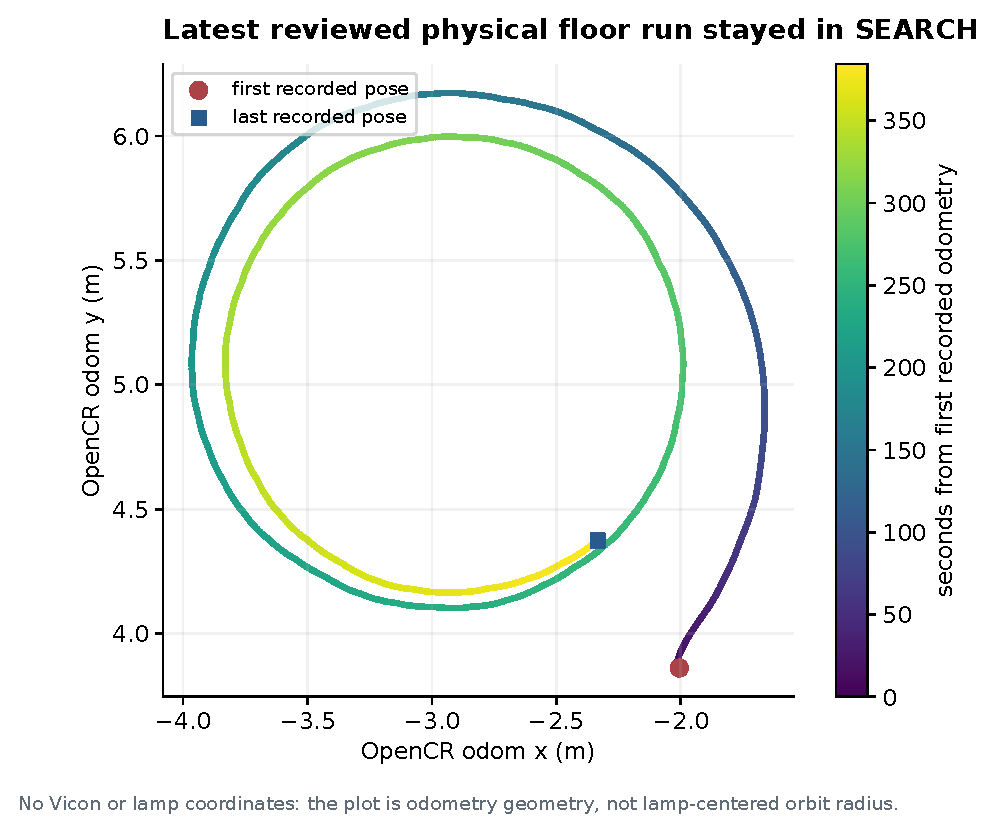
\includegraphics[width=0.85\linewidth,height=\textheight,keepaspectratio,alt={Latest reviewed physical floor run in OpenCR odometry. No lamp coordinates or Vicon measurements were available, so no lamp-centered radius is inferred.}]{v3/report_figures/physical_route.pdf}
\caption{Latest reviewed physical floor run in OpenCR odometry. No lamp
coordinates or Vicon measurements were available, so no lamp-centered
radius is inferred.}
\end{figure}

\subsection{Current physical boundary and proposed
continuation}\label{current-physical-boundary-and-proposed-continuation}

Physical deployment, native software/source/install/mirror checks and
six selected operator-observed raised-wheel stop tests are complete.
Physical \textbf{Gaussian fill, local escape and stronger-source
approach remain unqualified}. Full-graph loaded Pi headroom, deliberate
recoverable physical sensor interruption, quantified stopping latency
and OS/daemon/electrical faults are not established. Existing software
checks and selected continuous SEARCH do not close those boundaries.
{[}ES03, ES20-ES23, ES30, ES35{]}

The user's latest continuation preference is physical-led, simple and
reliable refinement; further Gazebo studies are not prerequisite work. A
reasonable controlled one-light comparison needs steady illumination,
repeatable start position/heading, known lamp
position/height/orientation and independent Vicon geometry before a
two-light escape test in adequate space. Proposed angular gain
\textbf{5.0\(\rightarrow\)7.5} and longer existing detector observation
windows remain \textbf{unapproved, undeployed and untested}. Current
physical angular gain is 5.0, caps 0.05/0.30. Raising angular cap alone
affected little of the latest run, which saturated angular command only
around 3\%. The ``escape should not take ten minutes'' concern is a
performance preference, not a new automatic timeout. {[}ES03, ES35{]}

Preserve the complete V1 backup, older failed V2
source/firmware/records, all run artifacts and the explicit V3
commissioning entrypoint. Do not promote V3 to the generic physical
Gaussian default or discard V1-specific dependency closure before
physical acceptance. Do not infer live Pi online/idle status from an
offline mirror or historical audit. The next physical trial remains
operator-controlled; this report itself authorizes no connection,
deployment, devices or motion. {[}ES03, ES20, ES21, ES24{]}

\subsection{Software validation receipts and reproduction without
rerunning
experiments}\label{software-validation-receipts-and-reproduction-without-rerunning-experiments}

{\def\LTcaptype{none} % do not increment counter
\begin{longtable}[]{@{}
  >{\raggedright\arraybackslash}p{(\linewidth - 4\tabcolsep) * \real{0.3000}}
  >{\raggedleft\arraybackslash}p{(\linewidth - 4\tabcolsep) * \real{0.4000}}
  >{\raggedright\arraybackslash}p{(\linewidth - 4\tabcolsep) * \real{0.3000}}@{}}
\toprule\noalign{}
\begin{minipage}[b]{\linewidth}\raggedright
Checkpoint
\end{minipage} & \begin{minipage}[b]{\linewidth}\raggedleft
Recorded passing checks
\end{minipage} & \begin{minipage}[b]{\linewidth}\raggedright
What it validates
\end{minipage} \\
\midrule\noalign{}
\endhead
\bottomrule\noalign{}
\endlastfoot
Refactor installed entrypoint suite & 196, no skips, 9.04 s & Active
runtime/installed profiles/interfaces, original numerics, isolated ROS
behavior \\
Initial Gazebo integration closeout & 228, no skips, 16.35 s & Clock
delivery, admission, signal and recorder fixes through that
checkpoint \\
Speed/lights/no-escape-deadline checkpoint & 240, no skips, 17.00 s &
Selected policy changes, late spatial completion, stale/stop integrity
behavior \\
Direct-assistance-disabled installed checkpoint & 249, no skips, 17.40 s
& Boolean selection plus prior active regressions \\
Affine-2.0 focused checks & 126, no skips, 2.51 s &
Coefficient/configuration plumbing and selected expectations; three
packages built \\
Physical deployment shared final suite & 297, 18.18 s & Shared physical
support/fault boundary/analysis at that stage \\
Worker correction & Host133 / Pi101 & Cold-import reproduction/fix and
installed actual-worker behavior \\
Steering correction & Host305 / Pi114 & Handoff freshness/context/reset,
priming and actual installed replay \\
Published Git closeout & 311, 21.23 s & Selected V3 regressions plus
deferred shutdown/light-marker checks at the published checkpoint \\
Report-date complete installed suite & \textbf{311, 21.81 s}, 372
warnings & Fresh current software verification on 2026-10-05; no
Gazebo/Pi/hardware run \\
\end{longtable}
}

Counts overlap and belong to distinct sources. They are not summed as
unique tests. Many inherited original NumPy matrix warnings, typically
372 at complete shared checkpoints, were reported; warnings were not
hidden or treated as research qualification. Report authoring did not
rerun expensive Gazebo/physical experiments merely to recover context.
The complete current installed software suite was rerun on 2026-10-05:
\textbf{311 passed, 372 inherited NumPy matrix warnings, 21.81 s}, with
finite timeout and localhost-only ROS tests, retained at
\path|report_20261005/current_software_tests.log|. This fresh
source/software verification launched no Gazebo or physical hardware.
{[}ES41{]} Read manifests, original bags, existing decoded CSV, retained
summaries/geometry/reviews and exact source snapshots first.
{[}ES12-ES19, ES22, ES23, ES29, ES38{]}

The exact retained final Git-checkpoint command, after ROS Humble and
the workspace overlay, was:

\begin{lstlisting}[language=bash]
ROS_LOCALHOST_ONLY=1 PYTHONDONTWRITEBYTECODE=1 timeout --signal=INT --kill-after=5s 150s python3 -m pytest -q -p no:cacheprovider ros2_ws/src/ros_esc/test/test_v3*.py ros2_ws/src/ros_esc/test/test_deferred_signal_shutdown.py ros2_ws/src/ros_esc/test/test_gazebo_light_markers.py
\end{lstlisting}

The report-date complete-suite verification used the following exact
command from the repository root (stdout/stderr retained in
\path|current_software_tests.log|):

\begin{lstlisting}[language=bash]
timeout 90s bash -c 'source /opt/ros/humble/setup.bash; source ros2_ws/install/setup.bash; export ROS_LOCALHOST_ONLY=1; python3 -m pytest -q ros2_ws/src/ros_esc/test --basetemp=/home/mattb/Experiments/GESC-Gaussian/v3/report_20261005/software_test_artifacts' > /home/mattb/Experiments/GESC-Gaussian/v3/report_20261005/current_software_tests.log 2>&1
\end{lstlisting}

This command records a software result, not a new Gazebo run. Physical
bag analysis can use the ordinary shared analyzer on a \textbf{closed}
bag; output topics absent from that bag remain unavailable. Do not
inspect an actively written SQLite bag and do not reuse consumed one-use
historical experiment launchers. Successful standard recording is a
durable observation source, not an automatic behavioral PASS. {[}ES21,
ES35, ES38{]}

For exact selected simulation figures, use
\path|affine_2_20260929T013558Z/analysis/csv/%2Fodom.csv|,
\path|%2Fgesc%2Fevents.csv| and \path|%2Fgesc%2Ffills.csv|, with
evaluator-only source coordinates from its captured
\passthrough{\lstinline!cost.json!}. For physical figures use
\path|physical_runs/20260930T211613_989126Z-3555/analysis/csv/%2Fodom.csv|
and \path|%2Fgesc%2Fobservation.csv|, explicitly labeling them OpenCR
odometry and host-receipt observations, with no lamp-distance or Vicon
claim. {[}ES18, ES19, ES35-ES37{]}

\subsection{Source references for these
chapters}\label{source-references-for-these-chapters}

\begin{itemize}
\item
  \textbf{ES01}:
  \href{/home/mattb/Experiments/GESC-Gaussian/v3/git_closeout_20261002T041241Z/final_receipt.json:1}{final\_receipt.json},
  lines 1-47. Current committed and published checkpoint; frozen refs;
  311 software checks.
\item
  \textbf{ES02}: \href{/home/mattb/dsim-lab/AGENTS.md:5}{AGENTS.md},
  lines 5-38. Active V3 authority and latest physical handoff priority.
\item
  \textbf{ES03}:
  \href{/home/mattb/dsim-lab/docs/codex/gesc_gaussian/v3/physical_fresh_chat_handoff.md:1}{physical\_fresh\_chat\_handoff.md},
  lines 1-194. Latest physical continuation, installed tuning,
  post-correction run, unapproved proposals.
\item
  \textbf{ES04}:
  \href{/home/mattb/dsim-lab/docs/codex/gesc_gaussian/v3/gazebo_status.md:622}{gazebo\_status.md},
  lines 622-718. Latest selected affine 2.0 simulation case and limits.
\item
  \textbf{ES05}:
  \href{/home/mattb/dsim-lab/docs/codex/gesc_gaussian/FINAL_PROJECT_REPORT_V1.md:57}{FINAL\_PROJECT\_REPORT\_V1.md},
  lines 57-104. Frozen V1 selected-case results and physical limit.
\item
  \textbf{ES06}:
  \href{/home/mattb/dsim-lab/docs/codex/gesc_gaussian/FINAL_PROJECT_REPORT_V1.md:681}{FINAL\_PROJECT\_REPORT\_V1.md},
  lines 681-745. Historic phase08 v3B/v3D suite naming and terminal
  selected V1 cases.
\item
  \textbf{ES07}:
  \href{/home/mattb/dsim-lab/docs/codex/gesc_gaussian/v2/fresh_chat_handoff.md:14}{fresh\_chat\_handoff.md},
  lines 14-92. Accepted TestD simulation and deferred historical bugs;
  later state annotated.
\item
  \textbf{ES08}:
  \href{/home/mattb/dsim-lab/docs/codex/gesc_gaussian/v2/low_rate_5hz_handoff.md:1}{low\_rate\_5hz\_handoff.md},
  lines 1-68. Selected V2 lowrate success with strict completenessFAIL
  and illconditioned fit.
\item
  \textbf{ES09}:
  \href{/home/mattb/dsim-lab/docs/codex/gesc_gaussian/v3/plan.md:1}{plan.md},
  lines 1-112. Initial V3 motivation and hardware timing facts;
  historical plan superseded.
\item
  \textbf{ES10}:
  \href{/home/mattb/dsim-lab/docs/codex/gesc_gaussian/v3/fault_inventory.md:1}{fault\_inventory.md},
  lines 1-74. Source-audit scope; unlike terminal faults; proposed
  simplification.
\item
  \textbf{ES11}:
  \href{/home/mattb/dsim-lab/docs/codex/gesc_gaussian/v3/refactor_plan.md:1}{refactor\_plan.md},
  lines 1-85. Accepted refactor topology, semantics and milestone
  authority.
\item
  \textbf{ES12}:
  \href{/home/mattb/dsim-lab/docs/codex/gesc_gaussian/v3/refactor_completion_audit.md:1}{refactor\_completion\_audit.md},
  lines 1-69. All nine refactor requirements; 196 tests; preserved
  archives and limits.
\item
  \textbf{ES13}:
  \href{/home/mattb/dsim-lab/docs/codex/gesc_gaussian/v3/gazebo_status.md:1}{gazebo\_status.md},
  lines 1-277. Runs01-05 outcomes; clock/signal/recorder corrections;
  software suites and model limits.
\item
  \textbf{ES14}:
  \href{/home/mattb/dsim-lab/docs/codex/gesc_gaussian/v3/gazebo_status.md:278}{gazebo\_status.md},
  lines 278-429. Speed/deadline/lights amendment; Run06 assisted
  success; final elapsed escape cutoff removal.
\item
  \textbf{ES15}:
  \href{/home/mattb/dsim-lab/docs/codex/gesc_gaussian/v3/gazebo_status.md:431}{gazebo\_status.md},
  lines 431-517. No-direct-assist selected pilot with affine0.5.
\item
  \textbf{ES16}:
  \href{/home/mattb/dsim-lab/docs/codex/gesc_gaussian/v3/gazebo_status.md:519}{gazebo\_status.md},
  lines 519-620. Tenfold affine5 experiment; source causal and
  saturation limits.
\item
  \textbf{ES17}:
  \href{/home/mattb/dsim-lab/docs/codex/gesc_gaussian/v3/gazebo_status.md:622}{gazebo\_status.md},
  lines 622-718. Selected affine2; actual chronology and comparison.
\item
  \textbf{ES18}:
  \href{/home/mattb/Experiments/GESC-Gaussian/v3/affine_2_20260929T013558Z/pilot_analysis.json:1}{pilot\_analysis.json},
  lines 1-1290. Exact selected bag decode, events, motion, source
  vicinity and fill diagnostics.
\item
  \textbf{ES19}:
  \href{/home/mattb/Experiments/GESC-Gaussian/v3/affine_2_20260929T013558Z/outcome_geometry.json:1}{outcome\_geometry.json},
  lines 1-1298. Independent recorded-odometry stableexit support,
  commands and descriptive proximity.
\item
  \textbf{ES20}:
  \href{/home/mattb/dsim-lab/docs/codex/gesc_gaussian/v3/physical_deployment_plan.md:1}{physical\_deployment\_plan.md},
  lines 1-148. Accepted physical milestone and amendments; next
  proposals unapproved.
\item
  \textbf{ES21}:
  \href{/home/mattb/dsim-lab/docs/esc_physical_v3.md:1}{esc\_physical\_v3.md},
  lines 1-135. Operator command, recovery, Vicon protocol, selected
  current settings and promotion boundary.
\item
  \textbf{ES22}:
  \href{/home/mattb/Experiments/GESC-Gaussian/v3/worker_init_20260930T215232Z/REVIEW.md:1}{REVIEW.md},
  lines 1-98. Cold import defect reproduction, installed correction,
  actual Pi replay, cache failure.
\item
  \textbf{ES23}:
  \href{/home/mattb/Experiments/GESC-Gaussian/v3/steering_handoff_20261001T040328Z/REVIEW.md:1}{REVIEW.md},
  lines 1-127. Accepted-snapshot handoff and initial priming mechanisms,
  tests, installed replay.
\item
  \textbf{ES24}:
  \href{/home/mattb/dsim-lab/docs/codex/gesc_gaussian/v3/physical_deployment_handoff.md:1}{physical\_deployment\_handoff.md},
  lines 1-182. Deployment archive hashes, ordinary workspace and
  preserved V1; dated state superseded.
\item
  \textbf{ES25}:
  \href{/home/mattb/physical_TB3_files_snapshot/pi/ros2_ws/src/turtlebot3_vehicle_nodes/turtlebot3_vehicle_nodes/v3_acquisition.py:1}{v3\_acquisition.py},
  lines 1-233. External offline source: physical acquisition, loop/pulse
  ownership and observation validity.
\item
  \textbf{ES26}:
  \href{/home/mattb/physical_TB3_files_snapshot/pi/ros2_ws/src/turtlebot3_vehicle_nodes/turtlebot3_vehicle_nodes/v3_acquisition_io.py:1}{v3\_acquisition\_io.py},
  lines 1-228. External offline source: negative voltage, fixed serial
  rate, finite framing, genuine edge age,54deg calibration.
\item
  \textbf{ES27}:
  \href{/home/mattb/physical_TB3_files_snapshot/pi/ros2_ws/src/turtlebot3_vehicle_nodes/turtlebot3_vehicle_nodes/v3_acquisition_observation.py:1}{v3\_acquisition\_observation.py},
  lines 1-46. External offline source: shared assembler
  radius/expiry/tolerance and unknown ADC uncertainty.
\item
  \textbf{ES28}:
  \href{/home/mattb/physical_TB3_files_snapshot/pi/ros2_ws/src/turtlebot3_vehicle_nodes/turtlebot3_vehicle_nodes/v3_runtime.py:1}{v3\_runtime.py},
  lines 1-340. External offline source:1s completed-loop and daemon
  lease; optional observers; local shutdown.
\item
  \textbf{ES29}:
  \href{/home/mattb/dsim-lab/docs/codex/gesc_gaussian/v3/physical_deployment_status.md:1}{physical\_deployment\_status.md},
  lines 1-121. Complete preservation, native deployment/legacy
  compatibility and ownership-stop review.
\item
  \textbf{ES30}:
  \href{/home/mattb/dsim-lab/docs/codex/gesc_gaussian/v3/physical_deployment_status.md:123}{physical\_deployment\_status.md},
  lines 123-194. Six raised-wheel checks; process exit measurements
  versus unmeasured stopping latency.
\item
  \textbf{ES31}:
  \href{/home/mattb/dsim-lab/docs/codex/gesc_gaussian/v3/physical_deployment_status.md:196}{physical\_deployment\_status.md},
  lines 196-247. Independent optional Vicon restoration and stationary
  proof.
\item
  \textbf{ES32}:
  \href{/home/mattb/dsim-lab/docs/codex/gesc_gaussian/v3/physical_deployment_status.md:249}{physical\_deployment\_status.md},
  lines 249-305. First mobile floor partial observation and authorized
  physical cap reduction.
\item
  \textbf{ES33}:
  \href{/home/mattb/Experiments/GESC-Gaussian/v3/physical_runs/night_20260929_review/REVIEW.md:1}{REVIEW.md},
  lines 1-194. Seven closed evening runs; SEARCHonly arcs, no detector
  candidates, reproduced cold-worker problem.
\item
  \textbf{ES34}:
  \href{/home/mattb/Experiments/GESC-Gaussian/v3/physical_runs/single_light_review_20261001T035033Z/REVIEW.md:1}{REVIEW.md},
  lines 1-144. Post-worker one-light recordings and distinct
  within-observation steering discontinuity.
\item
  \textbf{ES35}:
  \href{/home/mattb/Experiments/GESC-Gaussian/v3/physical_runs/post_steering_review_20261001T215339Z/REVIEW.md:1}{REVIEW.md},
  lines 1-142. Latest run detailed explanation, signal comparison,
  geometry gates and clock provenance.
\item
  \textbf{ES36}:
  \href{/home/mattb/Experiments/GESC-Gaussian/v3/physical_runs/post_steering_review_20261001T215339Z/metrics.json:1}{metrics.json},
  lines 1-107. Exact latest physical run metric values and event list.
\item
  \textbf{ES37}:
  \href{/home/mattb/Experiments/GESC-Gaussian/v3/physical_runs/post_steering_review_20261001T215339Z/detector_gate_counts.json:1}{detector\_gate\_counts.json},
  lines 1-9. Exact117 circle evaluations: both radius/coverage failed;
  no radial residual failures.
\item
  \textbf{ES38}:
  \href{/home/mattb/dsim-lab/docs/codex/gesc_gaussian/v3/physical_deployment_status.md:531}{physical\_deployment\_status.md},
  lines 531-558. Published source/doc closeout and exact311-check
  command; tuning unchanged.
\item
  \textbf{ES39}:
  \href{/home/mattb/physical_TB3_files_snapshot/pi/ros2_ws/src/ros_esc/config/profiles/assets/gesc_v3/controller.json:1}{controller.json},
  lines 1-19. Actual offline physical selected profile
  gains/caps/affine/optional assistance.
\item
  \textbf{ES40}:
  \href{/home/mattb/dsim-lab/docs/environment_parameters.md:1}{environment\_parameters.md},
  lines 1-45. Current V3 environment split; historical tables below are
  not active configuration.
\item
  \textbf{ES41}:
  \href{/home/mattb/Experiments/GESC-Gaussian/v3/report_20261005/current_software_tests.log:13}{current\_software\_tests.log},
  line 13. Fresh report-date complete installed software suite: 311
  passed, 372 warnings, 21.81 seconds; no Gazebo/Pi/hardware.
\end{itemize}

\section{Following one observation through the
code}\label{following-one-observation-through-the-code}

This walkthrough joins the earlier equations to their actual owners. Its
numerical values are an illustrative valid input, not a sample from a
retained trial. Suppose a new observation carries source time 10.000 s,
host receipt 10.020 s, a monotonically increasing host sequence, base
position (1.0, 2.0) m, yaw 30 degrees, relative arm phase 60 degrees,
and raw cost -1.20 V. The observed sensor position is (1.0, 2.18) m
because yaw plus phase is 90 degrees and the arm length is 0.18 m. The
raw voltage is positive 1.20 V; the minimization cost is negative. The
controller receives the independent current odometry as well as the
observation's associated pose.

At a control evaluation time of 10.040 s, source age is 0.040 s and ROS
receipt age is 0.020 s. The original local monotonic receipt age must
independently be within 0.5 s. Support ages must be no greater than 0.05
s. A duplicate sequence, older source time, frame conflict, or unusable
support changes the admission outcome; simply receiving a message is not
sufficient. A duplicate does not refresh the accepted reading's age.

Assume SEARCH is active, no fill exists, this is not the first accepted
reading, and the washout state before this sample is -1.18 V. The
augmented objective is therefore -1.20 V and the washed signal is -0.02
V. At phase 60 degrees, the instantaneous direction is

\[
q_b=-(-0.02)\frac{2}{0.18}
\begin{bmatrix}\cos60^\circ\\\sin60^\circ\end{bmatrix}
\approx\begin{bmatrix}0.1111\\0.1925\end{bmatrix}.
\]

If the source interval is 0.20 s and washout gain is 1 per second, the
next filter state becomes -1.184 V. The output above used -1.18 V, the
state before that update. Swapping that order changes the controller and
would no longer match the selected filter. The first sample of a new
core is handled differently: it seeds the washout state with the cost
and invents no initial gradient.

Rotate the body vector by the observation's yaw to obtain a world
vector. A qualified accepted rolling snapshot combines 75 percent cycle
mean with 25 percent instantaneous direction in its recorded context.
The current tick reprojects that world result with the current fresh
yaw. If no qualified mean is available, the fresh instantaneous
direction is the fallback. Completion of a coherence calculation retains
the original observation time; it does not make the result a new sample.

Using this example's instantaneous body vector alone, the ordinary
directional controller computes unsaturated commands

\[
v_x=0.5(0.1111)\approx0.0556\ \mathrm{m/s},\qquad
\omega_z=5(0.1925)\approx0.9623\ \mathrm{rad/s}.
\]

The Gazebo caps produce approximately (0.0556 m/s, 0.50 rad/s). The
physical caps produce (0.05 m/s, 0.30 rad/s). Both selected environments
use the same gain pair in V3. Saturating the angular component does not
proportionally rescale the linear component. A negative forward
component can produce reverse translation; the controller does not
normalize this estimate into a unit heading or replace it with an atan2
heading-error law.

Now imagine the independent odometry history qualifies recurrent
confinement. The detector nominates a center and the core starts VERIFY.
This does not immediately create a fill. The moving tracking law
approaches and samples around the candidate, while checking
neighborhood, actual displacement, input freshness, and actual
raw-sample angular coverage. Three comparable cycles can qualify raw
evidence. The candidate's sign/interval and the registry's existing fill
count determine whether to request a fill or compare sources.

In DESIGN, the controller freezes the sample and registry snapshots and
submits an immutable job to the worker. It continues the moving tracking
command while the proposal is computed. The result must match the
current candidate, epoch, objective and registry context. The main
controller applies an accepted change at a new actual source
observation, not by replaying this reading under a new objective. A job
timeout or failed residual-minimum test cancels the research attempt. It
does not make valid basic GESC control a terminal failure.

After the first fill is committed, ESCAPE evaluates the Gaussian and
affine functions at the measured sensor position and gives raw cost zero
weight. The same washout, direction and ordinary controller machinery
responds to that shaped objective. With direct assistance disabled,
there is no direct escape-heading pulse. Escape completion is measured
geometrically. The raw sensor objective is restored at a subsequent
actual observation, and the Gaussian remains to reduce attraction to the
visited basin.

The ROS node publishes \passthrough{\lstinline!/cmd\_vel!} and output
telemetry; the optional recorder can retain them with observations and
odometry. An analyst can compare command, measured motion, events and
fill geometry after the bag is closed. Command publication alone does
not establish that the robot moved or stopped.

Sources:
\path|ros2_ws/src/ros_esc/ros_esc/gesc_v3/core.py:119-242,329-442,463-570|;
\path|ros2_ws/src/ros_esc/ros_esc/gesc_v3/numerics/gesc.py:37-59|;
\path|ros2_ws/src/ros_esc/ros_esc/controller_node/controller_objects/turtlebot_vehicle.py:94-172|;
\path|ros2_ws/src/ros_esc/config/profiles/assets/gesc_v3/controller.json|.

\section{Explaining V3 to other
people}\label{explaining-v3-to-other-people}

\subsection{A short description for a general
audience}\label{a-short-description-for-a-general-audience}

Our robot searches for a stronger signal without knowing where the
sources are. A rotating sensor lets it compare signal changes around its
body and choose a direction. If the robot keeps revisiting a small
region, it checks the evidence while still moving. It can then add a
mathematical hill over that region and temporarily change its steering
objective so it leaves. After it gets out, it uses the measured signal
again. The selected simulation works satisfactorily; the physical
version is still being tested.

\subsection{A technical description for an
advisor}\label{a-technical-description-for-an-advisor}

V3 combines measured-phase gradient-descent extremum seeking with a
causal recurrent-motion detector, moving raw-cost verification, robust
local basin estimation and Gaussian cost shaping. Source-time
washout/demodulation produces instantaneous body-frame descent
estimates. Qualified rolling coherence blends a full-cycle world-frame
mean with instantaneous response. A local hybrid core coordinates
SEARCH, VERIFY, DESIGN and ESCAPE separately from command availability.
Gaussian preparation is computed in an isolated worker and committed
only in matching current context. During escape, raw attraction is
disabled and Gaussian plus affine guidance is minimized. Spatial
progress and exit evidence restore search. The current selected
implementation is a two-source, one-fill study, with a successful
unassisted Gazebo demonstration and physical SEARCH-only floor evidence.

\subsection{A software description for a new
collaborator}\label{a-software-description-for-a-new-collaborator}

The three ROS packages separate algorithm code, generated message
contracts, and Gazebo robot integration.
\passthrough{\lstinline!ros\_esc!} owns profiles, adapters, controllers,
the V3 core and analysis tools.
\passthrough{\lstinline!ros\_esc\_interfaces!} defines eight messages.
\path|turtlebot3_rotating_sensor| owns the simulation launch, model,
controllers and short method aliases. The original configurable
filter/controller path remains selectable. V3 uses the existing
controller entrypoint with \passthrough{\lstinline!--v3!}, one command
owner and one private numerical worker. Physical acquisition and process
stopping adapters live in the separate physical package, not in this
checkout. Runtime commands resolve installed profiles; they do not
silently rebuild the simulation workspace or rewrite configuration.

These descriptions deliberately keep measured success and intended
mechanism separate. If asked whether the robot knows which source is
global, explain the raw-interval comparison and the two-source
assumption. If asked whether the Gaussian changes the environment,
explain that it changes only the scalar function evaluated inside the
controller.

\section{Questions you should be able to
answer}\label{questions-you-should-be-able-to-answer}

\textbf{Why use a rotating sensor instead of one fixed sensor?} A scalar
reading at one point gives intensity, not a planar gradient. Known
spatial perturbation and measured phase make directional estimation
possible. The robot's moving base and nonuniform sampling make the
approximation imperfect; averaging and coherence assess usable evidence
rather than eliminating that limitation.

\textbf{Why is the voltage negated?} The selected controller minimizes
cost. A stronger light raises voltage, so negative voltage falls as
illumination rises. Changing that sign would steer the same estimator
toward lower illumination. Raw cost, augmented cost and source-ranking
evidence must keep their meanings.

\textbf{Why does demodulation contain 2 divided by arm length?} A
first-order spatial expansion has a directional signal proportional to
arm length. Averaging the outer product of a full circular unit
direction gives one half of the identity. The factor two compensates
that half, and dividing by length compensates the perturbation scale.
Measured sparse moving data only approximate the ideal derivation; it is
an explanation of the estimator, not an exact live gradient.

\textbf{Why wash out the absolute cost?} A constant brightness level
supplies no direction. The washout state tracks a slow baseline so the
modulated difference contains more of the directional variation. Initial
priming prevents one absolute reading from producing an invented startup
direction.

\textbf{Why can the robot reverse?} The forward command is proportional
to a signed body-frame direction component. The original numerical
controller preserves negative velocity. Reverse motion is allowed within
the selected caps; it is not automatically a failure. Actual motion
still has to satisfy the experiment.

\textbf{Why average in world coordinates?} Body coordinates turn with
the robot. Averaging body components across changing yaw can combine
different physical directions. Each vector is rotated to the observed
common frame before source-time integration; the final vector is
reprojected for current control.

\textbf{Does a full revolution mean the raw fill evidence is ready?}
No.~Steering and basin evidence have distinct contracts. Raw evidence
requires actual sector samples and multiple geometrically comparable
cycles. Interpolating a curve does not invent measured sectors or new
costs.

\textbf{Does a circle prove a light source is there?} No.~The detector
recognizes confined observed geometry. A robot can circle because of its
control law, space constraints or poor signal. Verification and source
comparison provide additional evidence, and the latest physical broad
orbit did not pass the selected detector's radius and angular-coverage
conditions.

\textbf{Why fit a quadratic if the final fill is a Gaussian?} The local
quadratic estimates gradient, curvature and model quality around the
basin. Kernel mean shift estimates the center, and spatial covariance
estimates observed spread. Together these inform Gaussian width,
amplitude and validation. The quadratic and covariance have different
roles and units; neither is a global field map.

\textbf{Why must amplitude and width be considered together?} At the
Gaussian center, curvature is proportional to negative amplitude times
inverse covariance. Increasing width at fixed amplitude lowers that
magnitude. A broad fill can cover more of a basin yet be too weak to
remove a modeled minimum. The designer tests the local augmented model
and can escalate width and amplitude together.

\textbf{Why add an affine term?} Gaussian repulsion is symmetric, has
zero gradient exactly at its center and decays away from it. A negative
linear slope supplies a consistent preferred escape direction. The
negative sign means minimization pushes along its vector. Its magnitude
is a cost slope, not a commanded speed.

\textbf{Is direct assistance the same as affine guidance?} No.~Affine
guidance changes the cost seen by GESC. Direct assistance substitutes a
latched direction for the ordinary steering estimate for one
measured-path pulse. The selected profile disables that pulse and still
uses Gaussian plus affine shaping during ESCAPE.

\textbf{Why use a worker?} Coherence quadrature and basin/fill
preparation can be expensive. Running them inside a control callback
risks delaying commands and freshness checks. A private process isolates
numerical work, limits one in-flight job, and returns data without
actuator or registry authority.

\textbf{Why can an old job finish successfully and still be rejected?}
It may answer a different candidate, objective revision, epoch or
registry generation, or have expired original data. Numerical success
says the calculation completed; context checks say whether its answer
still belongs to the live problem.

\textbf{Why not stop whenever recording fails?} A recorder is an
observer, not a control-input owner. Failure reduces retained evidence
and may make evaluation unavailable. It does not invalidate an otherwise
fresh direction and pose. The operator remains responsible for the
practical experiment.

\textbf{Why check a steady clock as well as simulated time?} A paused or
stalled Gazebo clock can freeze source-age arithmetic. Local monotonic
elapsed time continues, so unchanged input expires and the controller
commands zero. System/daemon/actuator failure is a different physical
question.

\textbf{Why not relax the detector radius to solve the physical orbit?}
A detector threshold observes motion; it does not change steering. The
latest replay also failed angular coverage, so a radius-only change
would not qualify its circles. First obtain controlled source-seeking
evidence and then evaluate detector recognition. The proposed angular
gain comparison remains undeployed.

\textbf{What exactly is accepted today?} The user accepts the
simulation/Gazebo development baseline. Software tests pass, and
selected Gazebo behavior supports unassisted escape and stronger-source
approach. Physical process-stop checks were observed under their stated
conditions, but physical fill and escape have not been established.
These are separate claims with separate evidence.

Sources: the mathematics, architecture and evidence chapters above and
their file-level citations. These answers summarize those checked
mechanisms; they do not introduce additional experimental claims.

\section{Study exercises with worked
answers}\label{study-exercises-with-worked-answers}

\begin{enumerate}
\def\labelenumi{\arabic{enumi}.}
\tightlist
\item
  \textbf{Cost sign.} A voltage changes from 0.40 to 1.10 V. Raw cost
  changes from -0.40 to -1.10 V, a decrease of 0.70 V. This is
  improvement for minimization. It does not by itself identify the
  global source.
\item
  \textbf{Body command.} A final body direction is (-0.08, 0.02). With
  gains 0.5/5, the command before caps is (-0.04 m/s, 0.10 rad/s). Both
  selected environments admit it. A negative first component commands
  reverse translation.
\item
  \textbf{Angular sampling.} Nominal 20 RPM is one revolution per 3 s.
  At 5 Hz, one revolution has about 15 samples and phase steps around 24
  degrees. Actual 17.07 RPM gives a period near 3.515 s and about 17.5
  samples per turn. Neither count guarantees a real sample in every
  selected sector when phase speed and delivery are nonuniform.
\item
  \textbf{Freshness.} A source reading is 0.60 s old but its worker
  result arrived 0.01 s ago. It is expired against the 0.5 s source
  limit. Result receipt does not renew it. A repeated old observation
  also fails to renew freshness.
\item
  \textbf{Gaussian value.} For amplitude 0.1 and isotropic sigma 0.5 m,
  the value at radius 0.5 m is about 0.06065, at 1.0 m about 0.01353,
  and at 1.5 m about 0.00111, in the objective's cost units. A declared
  support circle is a geometric convention; the Gaussian has an infinite
  mathematical tail.
\item
  \textbf{Affine sign.} Let the anchor be (0,0), direction (1,0), and
  magnitude 2. At (0.3,0), affine cost is approximately -0.6 at
  activation; at (-0.3,0), it is +0.6. Minimizing this term favors
  positive x. The magnitude 2 does not mean 2 m/s and remains subject to
  the ordinary controller caps.
\item
  \textbf{Circle evidence.} Two fitted arc radii 0.85 and 0.90 m fail
  the 0.5 m ceiling even if their centers barely drift. Radii 0.30 and
  0.32 m can still fail when either half covers only 40 degrees, below
  the 60-degree minimum. Passing one gate is insufficient for a circular
  nomination.
\item
  \textbf{Spatial exit.} For sigma 0.506211 m, support factor 3 yields
  1.518633 m and exit factor 2.7 yields 1.366770 m. The selected run
  values match those relationships. Being outside once is not the
  complete stable-exit predicate; progress history and exit hold still
  matter.
\item
  \textbf{Outcome versus event.} A retained trajectory is 0.0233 m from
  the modeled stronger source at its final pose, but contains no
  \passthrough{\lstinline!best\_source!} event. The correct statement is
  observed stronger-source vicinity without internal best-source
  confirmation. Do not rewrite either record to make them agree.
\item
  \textbf{Physical evidence.} A 382 s SEARCH-only run with a final zero
  exercises acquisition, steering and operator shutdown. It does not
  exercise Gaussian preparation or escape. Long duration cannot
  substitute for a missing state transition or an independent
  lamp-position measurement.
\end{enumerate}

These exercises use the selected equations and constants. The
walkthrough values are illustrative; the Gazebo and physical values are
identified as retained measurements in the evidence chapters.

\section{Evidence and source audit
appendices}\label{evidence-and-source-audit-appendices}

\subsection{File coverage and what complete means
here}\label{file-coverage-and-what-complete-means-here}

The companion \path|v3/report_coverage.tsv| contains 391 source/evidence
attributions across 285 distinct files. Each row records its role,
review mode, relevant line bounds, report section and SHA-256. The
architecture audit includes 232 distinct files; 141 were substantively
reviewed and 91 are explicitly inventory-only assets, examples, or
supporting modules. The mathematics audit adds 108 targeted
function/test attributions; the empirical audit adds 41 pinned records.
Overlap is deliberate: one file can support several claims. Counts are
coverage accounting, not numbers of independent experiments or tests.

The core, every active numerical module, selected profiles and JSON
resources, message schemas, launch/control/observation/worker owners,
relevant original method implementations and focused tests were
inspected for their substantive claims. CAD, meshes, example programs,
and historical duplicate experiments were inventoried when their
detailed contents were not needed to explain the active system. No claim
is made that every historical audio recording, binary CAD payload,
archived implementation or raw bag was reread byte by byte. Their
preserved locations and original report boundaries remain available.
This report is complete for the active V3 teaching and evidence scope,
rather than a new audit of every earlier experiment.

\path|v3/report_parameters.tsv| contains 839 attributed resource leaves
and runtime/default declarations. JSON-pointer keys identify nested
arrays and objects without collapsing symbolic filter expressions into
guessed numbers. Declared defaults, profile metadata, original-method
configurations, and actually consumed V3 settings are different
categories. The selected owner tables in the main text explain their
runtime effect. The TSV is a reference index, not a loader or additional
configuration source.

No algorithm source or physical tuning was changed for this report. The
fresh 311-test receipt verifies the audited local source/install on this
host. The prior Gazebo trial and latest physical trial keep their own
source snapshots, dates and limitations. Build and snapshot parity are
not hardware behavior.

\subsection{A compact file reading
map}\label{a-compact-file-reading-map}

{\def\LTcaptype{none} % do not increment counter
\begin{longtable}[]{@{}
  >{\raggedright\arraybackslash}p{(\linewidth - 2\tabcolsep) * \real{0.5000}}
  >{\raggedright\arraybackslash}p{(\linewidth - 2\tabcolsep) * \real{0.5000}}@{}}
\toprule\noalign{}
\begin{minipage}[b]{\linewidth}\raggedright
Question
\end{minipage} & \begin{minipage}[b]{\linewidth}\raggedright
Start at this active owner
\end{minipage} \\
\midrule\noalign{}
\endhead
\bottomrule\noalign{}
\endlastfoot
What does a run select? & \path|ros_esc/profiles.py|,
\path|config/profiles/algorithms.json|,
\passthrough{\lstinline!environments.json!}, selected controller/cost
JSON \\
Which processes exist? &
\path|turtlebot3_rotating_sensor/launch/gazebo.launch.py|,
\passthrough{\lstinline!ros\_esc/setup.py!} \\
What exactly is measured? & Eight \path|ros_esc_interfaces/msg/*.msg|
schemas; \path|gesc_v3/observation.py|, \path|observation_node.py|,
\passthrough{\lstinline!records.py!} \\
Who may issue a base command? &
\passthrough{\lstinline!gesc\_v3/node.py!},
\passthrough{\lstinline!core.py!},
\path|controller_node/controller_objects/turtlebot_vehicle.py| \\
What can run off-thread? & \passthrough{\lstinline!gesc\_v3/worker.py!},
immutable job keys, \passthrough{\lstinline!numerics/fill.py!} \\
Why does steering work this way? &
\passthrough{\lstinline!numerics/gesc.py!},
\passthrough{\lstinline!rolling.py!},
\passthrough{\lstinline!coherence.py!} \\
Why was a candidate recognized or rejected? &
\path|numerics/recurrent.py|, \passthrough{\lstinline!evidence.py!},
\passthrough{\lstinline!verification.py!},
\passthrough{\lstinline!core.py!} \\
What makes a Gaussian? & \passthrough{\lstinline!numerics/basin.py!},
\passthrough{\lstinline!fill\_design.py!},
\passthrough{\lstinline!registry.py!},
\passthrough{\lstinline!fill.py!} \\
What is the escape objective and exit rule? &
\path|numerics/objective.py|, \passthrough{\lstinline!escape.py!},
actual core call sites \\
What can the recording establish? & \path|run_tools/record_bag.py|,
\passthrough{\lstinline!analyze\_bag.py!}, closed run records and source
pins \\
Where did physical work stop? & \path|physical_fresh_chat_handoff.md|,
latest run REVIEW/metrics,
\passthrough{\lstinline!esc\_physical\_v3.md!} \\
\end{longtable}
}

Paths in this table are relative to the appropriate package root
described earlier; coverage rows give full paths. A function's presence
in a module is not evidence that the active core calls it. Follow the
call site, selected configuration, test and retained run before
describing a capability.

\subsection{Documentation drift discovered during the
audit}\label{documentation-drift-discovered-during-the-audit}

The root README's pre-deployment prose, the old nested message README,
historical environment tables, the superseded V3 planning status, and
retained helper comments are all dated descriptions. The main text
explains which statements are superseded and what current source does
instead. This report does not rewrite their historical outcomes. It also
does not promote the \passthrough{\lstinline!hb\_acoustic!} alias into
Heavy-Ball merely because of its label: the selected configuration is
what determines execution.

The V1 report set remains frozen. Its original links referring to
removed root shortcuts require the documented relocation mapping.
Historical Phase 08 v3A-D names are versions of a V1 experiment suite,
not the September V3 algorithm. Gaussian V1/V2 source remains on frozen
refs and in external archives. The original methods remain active and
selectable.

\subsection{Rebuilding the report and checking its
evidence}\label{rebuilding-the-report-and-checking-its-evidence}

The typeset source is reproducible from Markdown using
\path|v3/report_support/build_report.sh|, Pandoc 3.8.2.1 and Tectonic
0.17.0. The vector figure generator is
\path|v3/report_figures/generate_figures.py|; its two trajectory figures
require the exact retained closed CSV exports named in the validation
receipt. The other figures are explicitly explanatory schematics.
Neither script starts ROS, Gazebo, the Pi, or a physical device.

The final source/path, parameter, text, PDF structure, rendered-page and
Git checks are recorded in \path|v3/report_validation.md|. Large
renderer intermediates and test products stay in external experiment
storage. The report is a new documentation artifact and does not
constitute a new empirical milestone, new physical acceptance or
approval of undeployed gain/detector changes.

\end{document}
